\documentclass[11pt,reqno,a4letter]{article} 

\usepackage{amsmath,amssymb,amsfonts,amscd}

\usepackage{url}
\usepackage{hyperref}
\usepackage[usenames,dvipsnames]{xcolor}
\hypersetup{
    colorlinks,
    linkcolor={black!63!darkgray},
    citecolor={blue!70!white},
    urlcolor={blue!80!white}
}
\usepackage{graphicx} 

\newcommand{\hlocalref}[1]{\hyperref[#1]{\ref{#1}}}

\usepackage{datetime} 
\usepackage{cancel}
\usepackage{soul} 
\usepackage{subcaption}
\captionsetup{format=hang,labelfont={bf},textfont={small,it}} 
\numberwithin{equation}{section} 
\numberwithin{figure}{section}
\numberwithin{table}{section}

\usepackage{tocloft}
\usepackage{framed} 

\usepackage{enumitem}
\setlist[itemize]{leftmargin=0.65in}

\usepackage{changepage}
\usepackage{rotating,adjustbox}

\usepackage{diagbox}
\newcommand{\trianglenk}[2]{$\diagbox{#1}{#2}$}
\newcommand{\trianglenkII}[2]{\diagbox{#1}{#2}}

\let\citep\cite

\newcommand{\undersetbrace}[2]{\underset{\displaystyle{#1}}{\underbrace{#2}}}

\newcommand{\gkpSI}[2]{\ensuremath{\genfrac{\lbrack}{\rbrack}{0pt}{}{#1}{#2}}} 
\newcommand{\gkpSII}[2]{\ensuremath{\genfrac{\lbrace}{\rbrace}{0pt}{}{#1}{#2}}}
\newcommand{\cf}{\textit{cf.\ }} 
\newcommand{\Iverson}[1]{\ensuremath{\left[#1\right]_{\delta}}} 
\newcommand{\floor}[1]{\left\lfloor #1 \right\rfloor} 
\newcommand{\ceiling}[1]{\left\lceil #1 \right\rceil} 
\newcommand{\e}[1]{e\left(#1\right)} 
\newcommand{\seqnum}[1]{\href{http://oeis.org/#1}{\color{ProcessBlue}{\underline{#1}}}}

\usepackage{upgreek,dsfont,amssymb}
\renewcommand{\chi}{\upchi}
\newcommand{\ChiFunc}[1]{\ensuremath{\chi_{\{#1\}}}}
\newcommand{\OneFunc}[1]{\ensuremath{\mathds{1}_{#1}}}

%\usepackage{mathabx}
\makeatletter
\newcommand*\rel@kern[1]{\kern#1\dimexpr\macc@kerna}
\newcommand*\widebar[1]{%
  \begingroup
  \def\mathaccent##1##2{%
    \rel@kern{0.8}%
    \overline{\rel@kern{-0.8}\macc@nucleus\rel@kern{0.2}}%
    \rel@kern{-0.2}%
  }%
  \macc@depth\@ne
  \let\math@bgroup\@empty \let\math@egroup\macc@set@skewchar
  \mathsurround\z@ \frozen@everymath{\mathgroup\macc@group\relax}%
  \macc@set@skewchar\relax
  \let\mathaccentV\macc@nested@a
  \macc@nested@a\relax111{#1}%
  \endgroup
}

\usepackage{MnSymbol}
\newcommand{\gkpEII}[2]{\ensuremath{\genfrac{\llangle}{\rrangle}{0pt}{}{#1}{#2}}}

\usepackage{ifthen}
\newcommand{\Hn}[2]{
     \ifthenelse{\equal{#2}{1}}{H_{#1}}{H_{#1}^{\left(#2\right)}}
}

\newcommand{\Floor}[2]{\ensuremath{\left\lfloor \frac{#1}{#2} \right\rfloor}}
\newcommand{\Ceiling}[2]{\ensuremath{\left\lceil \frac{#1}{#2} \right\rceil}}

\DeclareMathOperator{\DGF}{DGF} 
\DeclareMathOperator{\ds}{ds} 
\DeclareMathOperator{\Id}{Id}
\DeclareMathOperator{\fg}{fg}
\DeclareMathOperator{\Div}{div}
\DeclareMathOperator{\rpp}{rpp}
\DeclareMathOperator{\logll}{\ell\ell}

\title{
       \LARGE{
       Exact formulas for partial sums of the M\"obius function expressed by 
       partial sums of weighted Liouville functions  
       } 
}
\author{{\Large Maxie Dion Schmidt} \\[0.1cm]  
        {\normalsize \href{mailto:maxieds@gmail.com}{maxieds@gmail.com}} \\[0.025cm] 
        {\normalsize \href{mailto:mschmidt34@gatech.edu}{mschmidt34@gatech.edu}} \\[0.025cm] 
        {\normalsize Georgia Institute of Technology} \\[0.025cm] 
        {\normalsize School of Mathematics} 
} 

%\date{\small\underline{Last Revised:} \today \ @\ \hhmmsstime{} \ -- \ Compiled with \LaTeX2e} 

\usepackage{amsthm} 

\theoremstyle{plain} 
\newtheorem{theorem}{Theorem}
\newtheorem{conjecture}[theorem]{Conjecture}
\newtheorem{claim}[theorem]{Claim}
\newtheorem{prop}[theorem]{Proposition}
\newtheorem{lemma}[theorem]{Lemma}
\newtheorem{cor}[theorem]{Corollary}
\numberwithin{theorem}{section}
\newtheorem*{conjecture*}{Conjecture}

\theoremstyle{definition} 
\newtheorem{example}[theorem]{Example}
\newtheorem{remark}[theorem]{Remark}
\newtheorem{definition}[theorem]{Definition}
\newtheorem{notation}[theorem]{Notation}
\newtheorem{question}[theorem]{Question}
\newtheorem{discussion}[theorem]{Discussion}
\newtheorem{facts}[theorem]{Facts}
\newtheorem{summary}[theorem]{Summary}
\newtheorem{heuristic}[theorem]{Heuristic}
\newtheorem{observation}[theorem]{Observation}
\newtheorem{ansatz}[theorem]{Ansatz}

\renewcommand{\arraystretch}{1.25} 
\usepackage[total={7in, 9.5in},tmargin=0.75in,headsep=8pt,footskip=30pt,footnotesep=0.5in]{geometry}

\usepackage{fancyhdr}
\pagestyle{empty}
\pagestyle{fancy}
\fancyhead[RO,RE]{Maxie Dion Schmidt -- \today} 
\fancyhead[LO,LE]{}
\fancyheadoffset{0.005\textwidth} 

\setlength{\parindent}{0em}
\setlength{\parskip}{2.5em} 

\renewcommand{\thefootnote}{\textbf{\arabic{footnote}}}

\renewcommand{\Re}{\operatorname{Re}}
\renewcommand{\Im}{\operatorname{Im}}

\usepackage{tikz}
\usetikzlibrary{shapes,arrows}

\usepackage{longtable}
\usepackage{arydshln} 
\usepackage[symbols,nogroupskip,nomain,automake=true,nonumberlist,section=section]{glossaries-extra}
\usepackage{glossary-mcols} 

\defglsdisplayfirst[main]{#1#4\protect\footnote{#2}}

%%%%%%%%%%%%

\providecommand{\glossarytoctitle}{\glossaryname}
\setlength{\glsdescwidth}{0.7\textwidth}

\newglossarystyle{glossstyleSymbol}{%
\renewenvironment{theglossary}%
 {\begin{longtable}{lp{\glsdescwidth}}}%
 {\end{longtable}}%
 \setlength{\parskip}{3.5pt}
 \renewcommand{\glsgroupskip}{}
\renewcommand*\glspostdescription{\dotfill}
\renewcommand*{\glossaryheader}{%
 \bfseries Symbols & \bfseries Definition
 \\\endhead}%
 \renewcommand*{\glsgroupheading}[1]{}%
  \renewcommand{\glossentry}[2]{%
    \glstarget{##1}{\glossentrysymbol{##1}} &
    \glossentrydesc{##1} \tabularnewline
  }%
  \renewcommand*{\glspostdescription}{}
  \renewcommand{\glossarymark}[1]{}
}

\setglossarystyle{glossstyleSymbol}
\makeglossaries

%%%%%%%%%%%%

\newglossaryentry{fCvlg}{
    symbol={\ensuremath{f \ast g}},
    sort={fg},
    description={The Dirichlet convolution of any two arithmetic functions 
    $f$ and $g$ at $n$ is defined to be 
    the divisor sum $(f \ast g)(n) := \sum\limits_{d|n} f(d) g\left(\frac{n}{d}\right)$ 
    for $n \geq 1$. 
    },
    type={symbols},
    name={Dirichlet convolution}
    }
\newglossaryentry{coeffExtraction}{
    symbol={\ensuremath{[q^n] F(q)}},
    sort={coeffExtraction},
    description={The coefficient of $q^n$ in the power series expansion of $F(q)$ about zero when 
    $F(q)$ is treated as the ordinary generating function (OGF) of a sequence, $\{f_n\}_{n \geq 0}$. 
    Namely, for integers $n \geq 0$ we define $[q^n] F(q) = f_n$ whenever 
    $F(q) := \sum\limits_{n \geq 0} f_n q^n$. },
    type={symbols},
    name={Series coefficient extraction}
    }
\newglossaryentry{MoebiusMuFunc}{
    symbol={\ensuremath{\mu(n),M(x)}},
    sort={MoebiusMuFunc},
    description={The M\"obius function defined such that $\mu^2(n)$ is the indicator function of the 
                 squarefree integers $n \geq 1$ where 
                 $\mu(n) = (-1)^{\omega(n)}$ whenever $n$ is squarefree. 
                 The Mertens function is the summatory function defined for all integers 
                 $x \geq 1$ by the partial sums $M(x) := \sum\limits_{n \leq x} \mu(n)$.
                 },
    type={symbols},
    name={M\"obius function}
    }
\newglossaryentry{Iverson}{
    symbol={\ensuremath{\Iverson{n=k}},\ensuremath{\Iverson{\mathtt{cond}}}},
    sort={Iverson},
    description={The symbol $\Iverson{n=k}$ is a synonym for $\delta_{n,k}$ 
                 which is one if and only if $n = k$, and is zero otherwise. 
                 For Boolean-valued conditions, \texttt{cond}, the symbol $\Iverson{\mathtt{cond}}$ 
                 evaluates to one precisely when \texttt{cond} is true or to zero otherwise.},
    type={symbols},
    name={Iverson's convention}
    }
\newglossaryentry{epsilonN}{
    symbol={\ensuremath{\varepsilon(n)}},
    sort={epsilonN},
    description={The multiplicative identity with respect to Dirichlet convolution, $\varepsilon(n) := \delta_{n,1}$, 
                 defined such that for any arithmetic function $f$ we have that 
                 $f \ast \varepsilon = \varepsilon \ast f = f$ where the operation 
                 $\ast$ denotes Dirichlet convolution. },
    type={symbols},
    name={Dirichlet multiplicative identity}
    }
\newglossaryentry{Zetas}{
    symbol={\ensuremath{\zeta(s)}},
    sort={Zetas},
    description={The Riemann zeta function is defined by 
                 $\zeta(s) := \sum\limits_{n \geq 1} n^{-s}$ when $\Re(s) > 1$, 
                 and by analytic continuation to any $s \in \mathbb{C}$ with the exception of a 
                 simple pole at $s = 1$ of residue one.},
    type={symbols},
    name={Riemann zeta function}
    }
\newglossaryentry{fInvn}{
     symbol={\ensuremath{f^{-1}(n)}},
    sort={fInvn},
    description={
     The Dirichlet inverse $f^{-1}$ of an arithmetic function $f$ exists 
     if and only if $f(1) \neq 0$. 
     The Dirichlet inverse of any $f$ such that $f(1) \neq 0$ 
     is defined recursively by 
     $f^{-1}(n) = -\frac{1}{f(1)} \times \sum\limits_{\substack{d|n \\ d>1}} f(d) f^{-1}\left(\frac{n}{d}\right)$ 
     for $n \geq 2$ with $f^{-1}(1) = f(1)^{-1}$. 
     When it exists, this inverse function 
     is unique and satisfies  $f^{-1} \ast f = f \ast f^{-1} = \varepsilon$.},
    type={symbols},
    name={Dirichlet inverse of $f$}
    }
\newglossaryentry{CkngInvAuxFunc}{
    symbol={$C_k(n),C_{\Omega}(n)$},
    sort={CkngInvAuxFunc},
    description={The first sequence is defined recursively for integers $n \geq 1$ and $k \geq 0$ as follows: 
                 \[
                 C_k(n) := \begin{cases} 
                      \delta_{n,1}, & \text{ if $k = 0$; } \\ 
                      \sum\limits_{d|n} \omega(d) C_{k-1}\left(\frac{n}{d}\right), & \text{ if $k \geq 1$. } 
                      \end{cases} 
                 \]
                 It represents the multiple ($k$-fold) convolution of the function $\omega(n)$ 
                 with itself. 
                 The function $C_{\Omega}(n) := C_{\Omega(n)}(n)$ has the DGF 
                 $(1-P(s))^{-1}$ for $\Re(s) > 1$. 
                 },
    type={symbols},
    name={Dirichlet inverse component functions}
    }
\newglossaryentry{gInvn}{
    symbol={$g(n),G(x),|G|(x)$},
    sort={gInvn},
    description={The Dirichlet inverse function, $g(n) = (\omega+1)^{-1}(n)$, has the 
                 summatory function $G(x) := \sum\limits_{n \leq x} g(n)$ for $x \geq 1$. 
                 We define the partial sums of the unsigned inverse function to be 
                 $|G|(x) := \sum_{n \leq x} |g(n)|$ for $x \geq 1$. },
    type={symbols},
    name={Key Dirichlet inverse functions}
    }
\newglossaryentry{PikPiHatkx}{
    symbol={$\pi_k(x),\widehat{\pi}_k(x)$},
    sort={PikPiHatkx},
    description={For integers $k \geq 1$, the 
                 function $\pi_k(x)$ denotes the number of 
                 $2 \leq n \leq x$ with 
                 exactly $k$ distinct prime factors: $\pi_k(x) := \#\{2 \leq n \leq x: \omega(n) = k\}$. 
                 Similarly, the function 
                 $\widehat{\pi}_k(x) := \#\{2 \leq n \leq x: \Omega(n) = k\}$ for $x \geq 2$ and fixed $k \geq 1$. },
    type={symbols},
    name={Distinct prime counting functions}
    }   
%\newglossaryentry{Nupn}{
%    symbol={$\nu_p(n)$}, 
%    sort={Nupn},
%    description={The valuation function that extracts the maximal exponent of $p$ in the prime factorization of $n$, e.g., 
%                 $\nu_p(n) = 0$ if $p \nmid n$ and $\nu_p(n) = \alpha$ if $p^{\alpha} || n$ 
%                 for $p \geq 2$ prime, $\alpha \geq 1$ and $n \geq 2$.},
%    type={symbols},
%    name={Exponent extraction function}
%    }
\newglossaryentry{primeOmegaFunctions}{
    symbol={$\omega(n)$,$\Omega(n)$}, 
    sort={OmegaPrimeOmegaFunctions},
    description={We define the strongly additive function 
                 $\omega(n) := \sum\limits_{p|n} 1$ and the completely additive function 
                 $\Omega(n) := \sum\limits_{p^{\alpha} || n} \alpha$. This means that if the prime 
                 factorization of any $n \geq 2$ is 
                 given by $n := p_1^{\alpha_1} \times \cdots \times p_r^{\alpha_r}$ 
                 with $p_i \neq p_j$ for all $i \neq j$, 
                 then $\omega(n) = r$ and $\Omega(n) = \alpha_1 + \cdots + \alpha_r$. 
                 We set $\omega(1) = \Omega(1) = 0$ by convention.},
    type={symbols},
    name={Prime omega functions}
    }
\newglossaryentry{LiouvilleLambdaFunc}{
     symbol={$\lambda(n), L(x)$}, 
    sort={LiouvilleLambdaFunc},
    description={The Liouville lambda function is the completely multiplicative function defined by 
                 $\lambda(n) := (-1)^{\Omega(n)}$. 
                 Its summatory function is defined by the partial sums 
                 $L(x) := \sum\limits_{n \leq x} \lambda(n)$ for $x \geq 1$. 
                 },
    type={symbols},
    name={Liouville lambda function}
    }
\newglossaryentry{QxSummatoryFunc}{
    symbol={$Q(x)$},
    sort={QxSummatoryFunc},
    description={For $x \geq 1$, we define $Q(x)$ to be the summatory function indicating the number of 
                 squarefree integers $n \leq x$. }, 
    type={symbols},
    name={Summatory function of the squarefree integers}
    }
\newglossaryentry{AApproxSimGGLLRelations}{
    symbol={$\gg,\ll,\asymp,\sim$},
    sort={AApproxSimGGLLRelations},
    description={
                 For functions $A,B$, the notation $A \ll B$ implies that $A = O(B)$. 
                 Similarly, for $B \geq 0$ the notation $A \gg B$ implies that $B = O(A)$. 
                 When we have that $A, B \geq 0$, $A \ll B$ and $B \ll A$, we write $A \asymp B$. 
                 Two arithmetic functions $A(x), B(x)$ satisfy the relation $A \sim B$ if 
                 $\lim_{x \rightarrow \infty} \frac{A(x)}{B(x)} = 1$. },
    type={symbols},
    name={Asymptotic relation symbols}
    }
%\newglossaryentry{NormalCDFFunc}{
%    symbol={$\Phi(z),\mathcal{N}(0,1)$},
%    sort={NormalCDFFunc},
%    description={For $z \in \mathbb{R}$, we take the cumulative density function (CDF) 
%                 of the standard normal distribution to be denoted by 
%                 $\Phi(z) := \frac{1}{\sqrt{2\pi}} \times \int\limits_{-\infty}^{z} e^{-\frac{t^2}{2}} dt$. 
%                 A random variable $Z$ whose values are distributed according to the CDF 
%                 $\Phi(z) = \mathbb{P}[Z \leq z]$ 
%                 has distribution denoted by $Z \sim \mathcal{N}(0, 1)$. },
%    type={symbols},
%    name={Asymptotic relation symbol}
%    }
\newglossaryentry{chiPrimeP}{
    symbol={$\chi_{\mathbb{P}}(n), P(s)$},
    sort={chiPrimeP},
    description={The indicator function of the primes equals one if and only if 
                 $n \in \mathbb{Z}^{+}$ is prime and is defined to be 
                 zero-valued otherwise. 
                 For any $s \in \mathbb{C}$ such that $\Re(s) > 1$, 
                 we define the prime zeta function to be the 
                 Dirichlet generating function (DGF) defined by 
                 $P(s) = \sum\limits_{n \geq 1} \frac{\chi_{\mathbb{P}}(n)}{n^s}$. 
                 The function $P(s)$ has an analytic continuation to the half-plane 
                 $\Re(s) > 0$ with the exception of $s = 1$ through the formula 
                 $P(s) = \sum\limits_{k \geq 1} \frac{\mu(k)}{k} \log\zeta(ks)$. The DGF $P(s)$ 
                 poles at the reciprocal of each positive integer and a natural boundary 
                 at the line $\Re(s) = 0$. },
    type={symbols},
    name={Prime set indicator function}
    }
\newglossaryentry{WLambertWFunction}{
    symbol={$W(x)$},
    sort={WLambertWFunction},
    description={For $x,y \in [0, +\infty)$, we write that $x = W(y)$ if and only if $xe^{x} = y$. 
                 This function denotes the principal branch of the multi-valued Lambert $W$ function 
                 taken over the non-negative reals. },
    type={symbols},
    name={Lambert $W$-Function}
    }
\newglossaryentry{GGTildeFHatGHatBivariateFunctions}{
    symbol={$\mathcal{G}(z),\widetilde{\mathcal{G}}(z)$; $\widehat{F}(s, z),\widehat{\mathcal{G}}(z)$},
    sort={GGTildeFHatGHatBivariateFunctions},
    description={The functions $\mathcal{G}(z)$ and $\widetilde{\mathcal{G}}(z)$ are defined for 
                 $0 \leq |z| \leq R < 2$ on page 
                 \pageref{subSection_TheKnownDistsOfThePrimeOmegaFunctions_IntroResults_v1} of 
                 Appendix \hlocalref{subSection_TheKnownDistsOfThePrimeOmegaFunctions_IntroResults_v1}. 
                 The related constructions 
                 used to motivate the definitions of 
                 $\widehat{F}(s, z)$ and $\widehat{\mathcal{G}}(z)$ are defined 
                 by the infinite products given on pages 
                 \pageref{prop_HatAzx_ModSummatoryFuncExps_RelatedToCkn} and 
                 \pageref{theorem_CnkSpCasesScaledSummatoryFuncs} of 
                 Section \hlocalref{subSection_Section4_AnalyticPrerequisiteProofsOfUniformBoundsOnCertainPartialSumTypes_v1}, 
                 respectively. },
    type={symbols},
    name={Bivariate DGFs}
    }
\newglossaryentry{GammaIncompleteGamma}{
    symbol={$\Gamma(a, z)$},
    sort={GammaIncompleteGamma},
    description={The incomplete gamma function is defined as $\Gamma(a, z) := \int_z^{\infty} t^{a-1} e^{-t} dt$ 
		 by continuation for $a \in \mathbb{R}$ and $|\operatorname{arg}(z)| < \pi$. } 
    type={symbols},
    name={Incomplete gamma function}
    }
%\newglossaryentry{ErrorFunctionsErfErfiz}{
%    symbol={$\operatorname{erf}(z),\operatorname{erfi}(z)$},
%    sort={ErrorFunctionsErfErfiz},
%    description={The function 
%                 $\operatorname{erf}(z)$ denotes the (ordinary) error function. It is related to the CDF, $\Phi(z)$, of the 
%                 standard normal distribution for any $z \in (-\infty, +\infty)$ through the 
%                 relation $\Phi(z) = \frac{1}{2}\left(1+\operatorname{erf}\left(\frac{z}{\sqrt{2}}\right)\right)$. 
%                 The imaginary error function is defined as 
%                 $\operatorname{erfi}(z) = \operatorname{erf}(\imath z) := 
%                  \frac{1}{\imath\sqrt{\pi}} \times \int_0^{\imath z} e^{t^2} dt$ for $z \in (-\infty, +\infty)$. 
%                 %An asymptotic series for these two functions as $|z| \rightarrow +\infty$ appears inline on 
%                 %page \pageref{cor_ExpectationFormulaAbsgInvn_v2} of 
%                 %Section \ref{subSection_AvgOrdersOfTheUnsignedSequences}. 
%                 },
%    type={symbols},
%    name={Error function variants}
%    }

\glsaddall[types={symbols}]

\allowdisplaybreaks 

\begin{document} 

\maketitle
\newcommand{\runtitle}{New exact formulas for partial sums of the M\"obius function}
\lhead{Maxie Dion Schmidt}
\rhead{\runtitle}

\begin{abstract} 
\noindent  
The Mertens function, $M(x) := \sum_{n \leq x} \mu(n)$, is 
defined as the summatory function of the classical M\"obius function for $x \geq 1$.
The Dirichlet inverse function $g(n) := (\omega+\mathds{1})^{-1}(n)$
is defined in terms of the shifted strongly additive function $\omega(n)$ that counts the 
number of distinct prime factors of $n$ without multiplicity. 
Discrete convolutions of the partial sums of $g(n)$ with the prime counting function 
provide new exact formulas for $M(x)$ that are weighted sums of the Liouville function 
involving $|g(n)|$ for $n \leq x$. 
We study the distribution of the unsigned function $|g(n)|$ through the auxiliary 
unsigned sequence $C_{\Omega}(n)$ whose Dirichlet generating function is given by 
$(1-P(s))^{-1}$ for $\Re(s) > 1$ where $P(s) = \sum_p p^{-s}$ is the 
prime zeta function. 
An application of the Selberg-Delange method yields asymptotics for the restricted sums 
of $C_{\Omega}(n)$ over all $n \leq x$ such that $\Omega(n)=k$ uniformly for 
$1 \leq k \leq \frac{3}{2} \log\log x$. 
We use these formulas to prove precise formulas for the average order of both 
$C_{\Omega}(n)$ and $|g(n)|$. 
Higher-order moments of these functions are predicted numerically by the conjecture 
that there is a limiting probability measure on $\mathbb{R}$ whose cumulative density function 
gives the distribution of the distinct values of each function over $n \leq x$ as 
$x \rightarrow \infty$. 

\bigskip 
\noindent
\textbf{Keywords and Phrases:} {\it M\"obius function; Mertens function; 
                                    Dirichlet inverse; Liouville lambda function; prime omega function; 
                                    prime counting function; Dirichlet generating function; 
                                    prime zeta function; Erd\H{o}s-Kac theorem. } \\ 
% 11-XX			Number theory
%    11A25  	Arithmetic functions; related numbers; inversion formulas
%    11Y70  	Values of arithmetic functions; tables
%    11-04  	Software, source code, etc. for problems pertaining to number theory
% 11Nxx		Multiplicative number theory
%    11N05  	Distribution of primes
%    11N37  	Asymptotic results on arithmetic functions
%    11N56  	Rate of growth of arithmetic functions
%    11N60  	Distribution functions associated with additive and positive multiplicative functions
%    11N64  	Other results on the distribution of values or the characterization of arithmetic functions
\textbf{Math Subject Classifications (2010):} {\it 11N37; 11A25; 11N60; 11N64; and 11-04. } 
\end{abstract} 

%\bigskip\hrule\medskip
%\begin{center}
%\begin{adjustwidth}{3.5cm}{}
%\emph{It is evident that the primes are randomly distributed but, \\ 
%        unfortunately, we do not know what 'random' means.} \\ 
%      \textbf{R. C. Vaughan} 
%\end{adjustwidth}
%\end{center}
%\medskip\hrule\bigskip

\newpage
\renewcommand{\contentsname}{Table of Contents}
\setcounter{tocdepth}{2}
\tableofcontents

\newpage
\section{Introduction} 
\label{subSection_MertensMxClassical_Intro} 
\label{example_InvertingARecRelForMx_Intro}

The Mertens function is the summatory function of $\mu(n)$ defined by the partial sums 
\cite[\seqnum{A008683}; \seqnum{A002321}]{OEIS} 
\begin{align} 
M(x) & = \sum_{n \leq x} \mu(n), \text{ for } x \geq 1. 
\end{align} 
The partial sums of the Liouville lambda function are defined by 
\cite[\seqnum{A008836}; \seqnum{A002819}]{OEIS}
\begin{equation}
\label{eqn_LxSummatoryFuncDef_v1}
L(x) := \sum\limits_{n \leq x} \lambda(n), \text{ for } x \geq 1. 
\end{equation}
The Mertens function is related to the partial sums in 
\eqref{eqn_LxSummatoryFuncDef_v1} 
via the relation \cite{HUMPHRIES-JNT-2013,LEHMAN-1960} 
\begin{equation}
\label{eqn_MxInTermsOfLx_v1} 
M(x) = \sum_{d \leq \sqrt{x}} \mu(d) L\left(\Floor{x}{d^2}\right), \text{ for } x \geq 1.
\end{equation}
We fix the notation for the Dirichlet inverse function \cite[\seqnum{A341444}]{OEIS} 
\begin{equation}
\label{eqn_gInvn_def_v1}
g(n) := (\omega + \mathds{1})^{-1}(n), \text{ for } n \geq 1. 
\end{equation}
We use the notation $|g(n)|$ to denote the absoute value of $g(n)$ where the sign of $g(n)$ is 
given by $\lambda(n)$ for all $n \geq 1$ 
(see Proposition \hlocalref{prop_SignageDirInvsOfPosBddArithmeticFuncs_v1}). 
We define the partial sums $G(x)$ for integers $x \geq 1$ as follows \cite[\seqnum{A341472}]{OEIS}: 
\begin{equation}
\label{eqn_GInvx_PartialSumForms_v1} 
G(x) := \sum_{n \leq x} g(n) = \sum_{n \leq x} \lambda(n) |g(n)|. 
\end{equation} 

\begin{theorem} 
\label{prop_Mx_SBP_IntegralFormula} 
\begin{subequations}
For all $x \geq 1$ 
\begin{align} 
\label{prop_Mx_SBP_IntegralFormula_PartA} 
M(x) & = G(x) + \sum_{1 \leq k \leq x} |g(k)| \pi\left(\Floor{x}{k}\right) \lambda(k), \\ 
\label{prop_Mx_SBP_IntegralFormula_PartB} 
M(x) & = G(x) + 
     \sum_{1 \leq k \leq \frac{x}{2}} \left(
     \pi\left(\Floor{x}{k}\right) - \pi\left(\Floor{x}{k+1}\right) 
	\right) G(k), \\ 
\label{eqn_RmkInitialConnectionOfMxToGInvx_ProvedByInversion_v1} 
M(x) & = G(x) + \sum_{p \leq x} G\left(\Floor{x}{p}\right). 
\end{align} 
\end{subequations}
\end{theorem}

The relation in \eqref{eqn_MxInTermsOfLx_v1} 
gives an exact expression for $M(x)$ with summands involving $L(x)$ that are oscillatory. 
In contrast, the exact expansions for the Mertens function given in 
Theorem \hlocalref{prop_Mx_SBP_IntegralFormula} 
express $M(x)$ as finite sums over $\lambda(n)$ with weight coefficients that are unsigned. 
For $n \geq 2$, let the function 
$\mathcal{E}[n] \vdash (\alpha_1, \alpha_2, \ldots, \alpha_r)$ denote the unordered 
partition of exponents for which 
$n = p_1^{\alpha_1} \times \cdots \times p_r^{\alpha_r}$ is the factorization of 
$n$ into powers of distinct primes. 
For any $n_1,n_2 \geq 2$ we have that 
\begin{equation}
\label{eqn_FactSymmPropertyOfgn_v1} 
\mathcal{E}[n_1] = \mathcal{E}[n_2] \implies g(n_1) = g(n_2). 
\end{equation}
The property of the symmetry of the distinct values of $|g(n)|$ with respect to the 
prime factorizations of $n \geq 2$ in \eqref{eqn_FactSymmPropertyOfgn_v1} 
shows \`{a} priori that the unsigned weights on $\lambda(n)$ in 
the new formulas from the theorem are comparatively easier to work with than prior 
exact expressions for $M(x)$ in terms of $L(x)$. 
Stating tight bounds on the distribution of 
$L(x)$ is a problem that is equally as difficult 
as understanding the properties of $M(x)$ well at large $x$ or 
along infinite subsequences (\cf \cite{MR2877066,MR3779960}). 

An exact expression for $g(n)$ is given by 
(see Lemma \hlocalref{lemma_AnExactFormulaFor_gInvByMobiusInv_v1} and 
Corollary \hlocalref{lemma_AbsValueOf_gInvn_FornSquareFree_v1}) 
\begin{equation}
\label{eqn_gInvn_ExactDivisorSumFormula_WithSgnWeight_v1} 
g(n) = \lambda(n) \times \sum_{d|n} \mu^2\left(\frac{n}{d}\right) C_{\Omega}(d), n \geq 1. 
\end{equation}
The sequence $\lambda(n) C_{\Omega}(n)$ has the 
Dirichlet generating function (DGF) $(1 + P(s))^{-1}$ and 
$C_{\Omega}(n)$ has the DGF $(1-P(s))^{-1}$ for $\Re(s) > 1$ 
where $P(s) := \sum_p p^{-s}$ is the prime zeta function. 
The function $C_{\Omega}(n)$ was considered in 
\cite{FROBERG-1968} with an exact formula 
given by \cite[\cf \S 3]{CLT-RANDOM-ORDERED-FACTS-2011} 
\begin{equation}
\label{eqn_proof_tag_hInvn_ExactNestedSumFormula_CombInterpetIdent_v3}
C_{\Omega}(n) = \begin{cases}
     1, & \text{if $n = 1$; } \\ 
     (\Omega(n))! \times \prod\limits_{p^{\alpha}||n} \frac{1}{\alpha!}, & \text{if $n \geq 2$. }
     \end{cases}
\end{equation} 
The focus of the article is on studying statistics of the unsigned functions 
$C_{\Omega}(n)$ and $|g(n)|$ and their partial sums. 
The new formulas for $M(x)$ given in 
Theorem \hlocalref{prop_Mx_SBP_IntegralFormula} 
provide a window from which we can view classically  
difficult problems about asymptotics for this function partially in terms of the 
properties of the auxiliary unsigned functions and their distributions. 

Define the function 
\[
\widehat{G}(z) := \frac{\zeta(2)^{-z}}{\Gamma(1+z) (1+P(2)z)}, \text{ for } 
     0 \leq |z| < P(2)^{-1} \approx 2.21118.
\]

\begin{theorem} 
\label{cor_SummatoryFuncsOfUnsignedSeqs_v2} 
For all sufficiently large $x$, there is an absolute constant $A_0 > 0$ such that 
uniformly for $1 \leq k \leq \frac{3}{2} \log\log x$  
\begin{align*} 
\sum_{\substack{n \leq x \\ \Omega(n)=k}} C_{\Omega}(n) & = 
     \frac{A_0 \sqrt{2\pi} x}{\log x} \times  
     \widehat{G}\left(\frac{k-1}{\log\log x}\right) 
     \frac{(\log\log x)^{k-\frac{1}{2}}}{(k-1)!} \left( 
     1 + O\left(\frac{1}{\log\log x}\right)\right). 
\end{align*} 
\end{theorem} 

We use Theorem \hlocalref{cor_SummatoryFuncsOfUnsignedSeqs_v2} with 
an adaptation of the form of Rankin's method from \cite[Thm.~7.20]{MV} 
to prove that for fixed $1 \leq r < P(2)^{-1}$ 
\[
\sum_{\substack{n \leq x \\ \Omega(n) \geq r \log\log x}} C_{\Omega}(n) \ll_r 
     x (\log x)^{r-1-r\log r} \sqrt{\log\log x}, \text{ as } 
     x \rightarrow \infty. 
\]
This result combined with the last theorem lead to a proof of the following 
average order formula: 

\begin{theorem} 
\label{lemma_HatCAstxSum_ExactFormulaWithError_v1} 
There is an absolute constant $B_0 > 0$ such that 
\[
\frac{1}{n} \times \sum_{k \leq n} C_{\Omega}(k) = 
B_0 \sqrt{\log\log n}\left(1 + O\left(\frac{1}{\log\log n}\right)\right), 
     \text{ as } n \rightarrow \infty. 
\] 
\end{theorem} 

The relation in \eqref{eqn_gInvn_ExactDivisorSumFormula_WithSgnWeight_v1} 
is used to deduce the average order of $|g(n)|$ from 
Theorem \hlocalref{lemma_HatCAstxSum_ExactFormulaWithError_v1}: 

\begin{theorem} 
\label{cor_ExpectationFormulaAbsgInvn_v2} 
As $n \rightarrow \infty$ 
\begin{align*} 
\frac{1}{n} \times \sum_{k \leq n} |g(k)| & = 
     \frac{6B_0 (\log n) \sqrt{\log\log n}}{\pi^2} 
     \left(1 + O\left(\frac{1}{\log\log n}\right)\right). 
\end{align*} 
\end{theorem} 

\begin{conjecture*}
There are explicit unbounded monotone increasing functions, 
$\mu_{\Omega}(x)$ and $\sigma_{\Omega}(x)$, and 
a limiting probability measure, $\phi_{\Omega}$, on $\mathbb{R}$ with 
associated cumulative density function given by $\Phi_{\Omega}$ so that 
for any $y \in (-\infty, +\infty)$ 
\begin{align*} 
\frac{1}{x} \times \#\left\{3 \leq n \leq x: \frac{|g(n)| - 
	\frac{1}{n} \times \sum_{k \leq n} |g(k)| - \frac{6}{\pi^2} \mu_{\Omega}(x)}{\sigma_{\Omega}(x)}  
     \leq y\right\} & = 
     \Phi_{\Omega}\left(\frac{\pi^2 y}{6}\right) + o(1), \text{ as } x \rightarrow \infty. 
\end{align*}
\end{conjecture*}

The article is organized into sections that prove our new results for each of the functions 
$C_{\Omega}(n)$, $g(n)$ and $|g(n)|$, and then establish the proofs of the 
exact formulas for $M(x)$ stated in 
Theorem \hlocalref{prop_Mx_SBP_IntegralFormula}. 
The appendix sections provide a glossary of notation and 
supplementary material on topics that can be separated from the 
organization in the main sections of the article. 

\section{An asymptotic formula for certain partial sums}

This section proves in 
Theorem \hlocalref{prop_HatAzx_ModSummatoryFuncExps_RelatedToCkn} 
an asymptotic analysis of the generating function $\widehat{A}_z(x)$ 
given by the next definition. The formula proved in the theorem is 
used to prove the results in 
Section \hlocalref{Section_NewFormulasForgInvn_v1} which then in turn 
lead to proofs of the results on the inverse function $g(n)$ in 
Section \hlocalref{Section_NewFormulasForgInvn_v2}. 

\begin{definition}
\label{def_PartialSumsOfCvlFunc_HatAzx_v1} 
For any $x \geq 1$ we define the partial sums 
\[
\widehat{A}_z(x) := \sum_{n \leq x} (-1)^{\omega(n)} 
     C_{\Omega}(n) z^{\Omega(n)}. 
\]
The function is $C_{\Omega}(n)$ defined in equation 
\eqref{eqn_proof_tag_hInvn_ExactNestedSumFormula_CombInterpetIdent_v3} 
of the introduction (see 
Section \hlocalref{Section_NewFormulasForgInvn_v1}). 
\end{definition}

The asymptotic analysis will be obtained via study of the following 
Dirichlet generating function (DGF):

\begin{definition}
\label{def_BivariateDGF_HatFsz_AndRelatedFuncs_v1}
Let the bivariate DGF $\widehat{F}(s, z)$ be defined 
for $\Re(s) > 1$ and $|z| < |P(s)|^{-1}$ by 
\[
\widehat{F}(s, z) := \frac{1}{1+P(s) z} 
     \times \prod_p \left(1 - \frac{1}{p^s}\right)^{z} = 
     \frac{\zeta(s)^{-z}}{1+P(s) z}. 
\]
We define the $z$-dependent sequence of coefficients $\{b_z(n)\}_{n \geq 1}$ in the 
series expansion of the DGF 
\[
\widehat{F}(s, z) \zeta(s)^{z} = \sum_{n \geq 1} \frac{b_z(n)}{n^s}, \text{ for } 
     \Re(s) > 1 \text{ and } |z| < |P(s)|^{-1}. 
\]
For any $0 \leq |z| < P(2)^{-1}$ we define the function 
\begin{equation}
\label{eqn_def_HatGz_v2}
\widehat{G}(z) := \frac{\widehat{F}(2, z)}{\Gamma(1+z)}. 
\end{equation}
\end{definition}

The function $\widehat{A}_z(x)$ is obtained as the partial sums of the coefficients of the DGF 
$\widehat{F}(s, z)$ when $s := 2$ 
(see equation \eqref{eqn_proof_tag_Azx_FullTermsFormulaSum_v1} in the proof below). 
The Dirichlet generating function $\widehat{F}(s, z)$ can be studied through the 
Selberg-Delange method presented in Tenebaum \cite[\S II.6.1]{TENENBAUM-PROBNUMT-METHODS} 
(see also \cite[\cf \S 7.4]{MV}).
\begin{subequations}
In particular, we define the coefficients $\{d_z(n)\}_{n \geq 1}$ in the DGF of comoplex-valued powers of the 
Riemann zeta function by the series expansion 
\begin{equation}
\label{eqn_Dzx_PartialSumsInSelbergDelangeMethod_v0} 
\zeta(s)^z = \sum_{n \geq 1} \frac{d_z(n)}{n^s}, \text{ for } \Re(s) > 1 \text{ and } z \in \mathbb{C}. 
\end{equation}
Asymptotics for the partial sums 
\begin{equation}
\label{eqn_Dzx_PartialSumsInSelbergDelangeMethod_v1} 
D_z(x) := \sum_{n \leq x} d_z(n), \text{ for } x \geq 1 \text{ and } z \in \mathbb{C}, 
\end{equation}
require careful evaluation via a Hankel loop contour over $\zeta(s)^z$ for 
general complex $z \in \mathbb{C} \setminus \mathbb{Q}$. 
We have that \cite[Thm.\ 7.17; \S 7.4]{MV}
\begin{equation}
\label{eqn_Dzx_PartialSumsInSelbergDelangeMethod_v2} 
D_z(x) = \frac{x (\log x)^{z-1}}{\Gamma(z)} + O_z\left(x (\log x)^{\Re(z)-2}\right), 
     \text{ for } x \geq 2 \text{ and } 0 < |z| < 2. 
\end{equation}
\end{subequations}
The analysis given in Tenenbaum's work is not sufficient for our application, because in our case here, 
the auxiliary variable z is introduced, and eventually we specify that $s := 2$ 
(as opposed to taking $s := 1$ in Selberg's original proof \cite{SELBERG-NOTE-SATHE}).

\begin{theorem} 
\label{prop_HatAzx_ModSummatoryFuncExps_RelatedToCkn} 
For all sufficiently large $x \geq 2$ and $|z|< 2$ 
\[
\widehat{A}_z(x) = \frac{x \widehat{F}(2, z)}{\Gamma(z)} (\log x)^{z-1} + 
     O_{z}\left(x (\log x)^{\Re(z) - 2}\right). 
\]
\end{theorem} 
\begin{proof} 
It follows from \eqref{eqn_proof_tag_hInvn_ExactNestedSumFormula_CombInterpetIdent_v3} that 
we can generate exponentially scaled forms of the function $C_{\Omega}(n)$ by 
a product identity of the following form: 
\begin{align*} 
\sum_{n \geq 1} \frac{C_{\Omega}(n)}{(\Omega(n))!} \cdot 
     \frac{(-1)^{\omega(n)} z^{\Omega(n)}}{n^s} & = \prod_p \left(1 + \sum_{r \geq 1} 
     \frac{z^{\Omega(p^r)}}{r! p^{rs}}\right)^{-1} 
     = \exp\left(-z P(s)\right), \text{ for } \Re(s) > 1 \text{ and } \Re(P(s)z) > -1. 
\end{align*} 
This Euler product type expansion is similar in construction to the parameterized bivariate 
DGFs defined in \cite[\S 7.4]{MV} \cite[\cf \S II.6.1]{TENENBAUM-PROBNUMT-METHODS}.
By computing a termwise Laplace transform applied to the right-hand-side of the 
previous equation, we obtain that 
\begin{align*} 
\sum_{n \geq 1} \frac{C_{\Omega}(n) (-1)^{\omega(n)} z^{\Omega(n)}}{n^s} & = 
     \int_0^{\infty} e^{-t} \exp\left(-tz P(s)\right) dt = \frac{1}{1 + P(s) z}, 
     \text{ for } \Re(s) > 1 \text{ and } \Re(P(s)z) > -1. 
\end{align*} 
It follows from the Euler product representation of $\zeta(s)$, which is convergent for any 
$\Re(s) > 1$, that 
\begin{align}
\widehat{F}(s, z) \zeta(s)^{z} & = \sum_{n \geq 1} \frac{(-1)^{\omega(n)} C_{\Omega}(n) z^{\Omega(n)}}{n^s} 
     = \frac{1}{1 + P(s) z}, 
     \text{ for } \Re(s) > 1 \text{ and } |z| < |P(s)|^{-1}. 
\end{align}
The DGF $\widehat{F}(s, z)$ is an analytic function of $s$ for all $\Re(s) > 1$ 
whenever the parameter $|z| < |P(s)|^{-1}$. 
Indeed, whenever $|z| \leq R < |P(s)|^{-1}$ 
\[
\left\lvert \sum_{n \geq 1} \frac{b_z(n) (\log n)^{2R+1}}{n^s} \right\rvert < +\infty. 
\]
Moreover, the series in the last equation is uniformly bounded for all $\Re(s) \geq 2$ and 
$|z| \leq R < |P(s)|^{-1}$. 

For fixed $0 < |z| < 2$, the sequence $\{d_z(n)\}_{n \geq 1}$ 
is defined as in \eqref{eqn_Dzx_PartialSumsInSelbergDelangeMethod_v0}. 
An asymptotic formula for its partial sums, $D_z(x)$, whenever $x \geq 2$ is given in 
\eqref{eqn_Dzx_PartialSumsInSelbergDelangeMethod_v2}. 
Let $b_z(n) := (-1)^{\omega(n)} C_{\Omega}(n) z^{\Omega(n)}$ (in agreement with 
Definition \hlocalref{def_BivariateDGF_HatFsz_AndRelatedFuncs_v1}) and  
take the convolution sequence 
$$\hat{a}_z(n) := \sum\limits_{d|n} b_z(d) d_z\left(\frac{n}{d}\right), \text{ for } n \geq 1.$$  
The partial sums $\widehat{A}_z(x)$ from 
Definition \hlocalref{def_PartialSumsOfCvlFunc_HatAzx_v1} are given by 
$$\widehat{A}_z(x) := \sum\limits_{n \leq x} \hat{a}_z(n).$$ 
Then we have that for any $0 < |z| < 2$ 
\begin{align} 
\notag 
\widehat{A}_z(x) & = \sum_{m \leq \frac{x}{2}} b_z(m) D_z\left(\frac{x}{m}\right) + 
     \sum_{\frac{x}{2} < m \leq x} b_z(m) \\ 
\label{eqn_proof_tag_Azx_FullTermsFormulaSum_v1} 
     & = \frac{x}{\Gamma(z)} \times \sum_{m \leq \frac{x}{2}} 
     \frac{b_z(m)}{m} \log\left(\frac{x}{m}\right)^{z-1} + 
     O\left(\sum_{m \leq x} \frac{x |b_z(m)|}{m} \times
     \log\left(\frac{2x}{m}\right)^{\Re(z) - 2}\right). 
\end{align} 
We can sum the coefficients $\frac{b_z(m)}{m}$ 
for integers $m \leq u$ when $u$ is taken sufficiently large as 
\begin{align*} 
\sum_{1 \leq m \leq u} \frac{b_z(m)}{m^2} \times m & = \widehat{F}(2, z) + O_z\left(u^{-1}\right). 
\end{align*} 
Suppose that $0 < |z| \leq R < 2$. 
For large $x$, the error term in \eqref{eqn_proof_tag_Azx_FullTermsFormulaSum_v1} satisfies 
\begin{align*} 
\sum_{m \leq x} \frac{x |b_z(m)|}{m} 
     \log\left(\frac{2x}{m}\right)^{\Re(z) - 2} & \ll 
     x (\log x)^{\Re(z) - 2} \times \sum_{m \leq \sqrt{x}} \frac{|b_z(m)|}{m} + 
     x (\log x)^{-(R+2)} \times \sum_{m > \sqrt{x}} \frac{|b_z(m)|}{m} (\log m)^{2R}, \\ 
     & = O_z\left(x (\log x)^{\Re(z) - 2}\right). 
\end{align*} 
When $m \leq \sqrt{x}$ we have that 
\[
\log\left(\frac{x}{m}\right)^{z-1} = (\log x)^{z-1} + 
     O\left((\log m) (\log x)^{\Re(z) - 2}\right). 
\]
A related bound is obtained for the left-hand-side of the previous equation 
expanding in powers of $\log m$ 
when $\sqrt{x} < m < x$ and $0 < |z| < R$. 
The combined sum over the interval $m \leq \frac{x}{2}$ produces the following bounds 
when $0 < |z| \leq R$: 
\begin{align*} 
\sum_{m \leq \frac{x}{2}} b_z(m) D_z\left(\frac{x}{m}\right) & = \frac{x}{\Gamma(z)} (\log x)^{z-1} \times 
     \sum_{m \leq \frac{x}{2}} \frac{b_z(m)}{m} \\ 
     & \phantom{=\quad\ } + 
     O_R\left(x (\log x)^{\Re(z)-2} \times \sum_{m \leq \sqrt{x}} \frac{|b_z(m)| \log m}{m} + 
     x (\log x)^{R-1} \times \sum_{m > \sqrt{x}} \frac{|b_z(m)|}{m}\right) \\ 
     & = \frac{x \widehat{F}(2, z)}{\Gamma(z)} (\log x)^{z-1} + O_R\left( 
     x (\log x)^{\Re(z)-2} \times \sum_{m \geq 1} \frac{b_z(m) (\log m)^{2R+1}}{m^2} 
     \right) \\ 
     & = \frac{x \widehat{F}(2, z)}{\Gamma(z)} (\log x)^{z-1} + O_{R}\left( 
     x (\log x)^{\Re(z)-2}\right). 
     \qedhere  
\end{align*} 
\end{proof} 

\section{Properties of the function $C_{\Omega}(n)$} 
\label{Section_NewFormulasForgInvn_v1} 

The function $C_{\Omega}(n)$ is key to understanding the 
unsigned inverse sequence $|g(n)|$. In this section, we define $C_{\Omega}(n)$ 
precisely and explore its properties. 

\begin{definition}
We define the following bivariate sequence for integers $n \geq 1$ and $k \geq 0$: 
\begin{align} 
\label{eqn_CknFuncDef_v2} 
C_k(n) := \begin{cases} 
     \varepsilon(n), & \text{ if $k = 0$; } \\ 
     \sum\limits_{d|n} \omega(d) C_{k-1}\left(\frac{n}{d}\right), & \text{ if $k \geq 1$. } 
     \end{cases} 
\end{align} 
Using the notation for iterated convolution in 
Bateman and Diamond \cite[Def.~ 2.3; \S 2]{ANT-BATEMAN-DIAMOND} we have 
$C_0(n) \equiv \omega^{\ast 0}(n)$ and $C_k(n) \equiv \omega^{\ast k}(n)$ for 
integers $k \geq 1$ and $n \geq 1$. 
The special case of \eqref{eqn_CknFuncDef_v2} where 
$k := \Omega(n)$ occurs frequently in the next sections of the 
article. To avoid cumbersome notation when referring to this common function variant, we suppress the 
duplicate index $n$ by writing $C_{\Omega}(n) := C_{\Omega(n)}(n)$ \cite[\seqnum{A008480}]{OEIS}. 
\end{definition}

\begin{remark}
By recursively expanding the definition of $C_k(n)$ 
at any fixed $n \geq 2$, we see that 
we can form a chain of at most $\Omega(n)$ iterated (or nested) divisor sums by 
unfolding the definition of \eqref{eqn_CknFuncDef_v2} inductively. 
By the same argument, we see that at fixed $n$, the function 
$C_k(n)$ is non-zero only possibly for 
$1 \leq k \leq \Omega(n)$ when $n \geq 2$. 
We see by 
\eqref{eqn_proof_tag_hInvn_ExactNestedSumFormula_CombInterpetIdent_v3} 
that $C_{\Omega}(n) \leq (\Omega(n))!$ for all $n \geq 1$ with 
equality precisely at the squarefree integers so that 
$(\Omega(n))! = (\omega(n))!$ whenever $\mu^2(n) = 1$. 
\end{remark}

\subsection{Uniform asymptotics for partial sums}
\label{subSection_Section4_AnalyticPrerequisiteProofsOfUniformBoundsOnCertainPartialSumTypes_v1} 

\begin{definition}
For integers $x \geq 3$ and $k \geq 1$, two variants of the 
restricted partial sums of the function $C_{\Omega}(n)$ are defined as follows: 
\begin{align*} 
\widehat{C}_{k,\omega}(x) & := \sum_{\substack{n \leq x \\ \Omega(n) = k}} 
     (-1)^{\omega(n)} C_{\Omega}(n), \\ 
\widehat{C}_k(x) & := \sum_{\substack{n \leq x \\ \Omega(n) = k}} C_{\Omega}(n). 
\end{align*}
\end{definition}

Recall that we have defined the function 
$\widehat{G}(z) := \widehat{F}(2, z) \times \Gamma(1+z)^{-1}$ for any $0 \leq |z| < P(2)^{-1}$ in 
Definition \hlocalref{def_BivariateDGF_HatFsz_AndRelatedFuncs_v1} 
of the previous section. 

\begin{theorem} 
\label{theorem_CnkSpCasesScaledSummatoryFuncs} 
As $x \rightarrow \infty$, uniformly for $1 \leq k \leq 2\log\log x$ 
\[
\widehat{C}_{k,\omega}(x) = -\widehat{G}\left(\frac{k-1}{\log\log x}\right) \frac{x}{\log x} \cdot 
     \frac{(\log\log x)^{k-1}}{(k-1)!} \left( 
     1 + O\left(\frac{k}{(\log\log x)^2}\right)\right). 
\]
\end{theorem} 
\begin{proof} 
When $k = 1$, we have that $\Omega(n) = \omega(n)$ for all $n \leq x$ such that $\Omega(n) = k$. 
The positive integers $n$ that satisfy this requirement are precisely the primes $p \leq x$. 
The formula is satisfied as 
\[
\sum_{p \leq x} (-1)^{\omega(p)} C_{\Omega}(p) = -\sum_{p \leq x} 1 = 
     - \frac{x}{\log x} \left(1 + O\left(\frac{1}{\log x}\right)\right). 
\]
%Since $O\left((\log x)^{-1}\right) = O\left((\log\log x)^{-2}\right)$ as 
%$x \rightarrow \infty$, we obtain the required error term for the bound at $k = 1$. 
For $2 \leq k \leq 2\log\log x$, we will apply the error estimate from 
Theorem \hlocalref{prop_HatAzx_ModSummatoryFuncExps_RelatedToCkn} with 
$r := \frac{k-1}{\log\log x}$ to
\[
\widehat{C}_{k,\omega}(x) = \frac{(-1)^{k+1}}{2\pi\imath} \times \int_{|v|=r} 
     \frac{\widehat{A}_{-v}(x)}{v^{k+1}} dv. 
\]
The error in this formula 
contributes terms that are bounded by 
\begin{align*} 
\left\lvert x (\log x)^{-(\Re(v)+2)} v^{-(k+1)} \right\rvert & \ll 
     \left\lvert x (\log x)^{-(r+2)} r^{-(k+1)} \right\rvert 
     \ll \frac{x}{(\log x)^{2-\frac{k-1}{\log\log x}}} \cdot 
     \frac{(\log\log x)^{k}}{(k-1)^{k}} \\ 
     & \ll \frac{x}{(\log x)^2} \cdot \frac{(\log\log x)^{k+1}}{(k-1)^{\frac{1}{2}} (k-1)!} 
     \ll \frac{x}{\log x} \cdot \frac{k (\log\log x)^{k-5}}{(k-1)!}, 
     \text{ as } x \rightarrow \infty. 
\end{align*} 
We next find the main term for the coefficients 
of the following contour integral when 
$r \in [0, z_{\max}] \subseteq \left[0, P(2)^{-1}\right)$: 
\begin{align} 
\label{eqn_WideTildeArx_CountourIntDef_v1} 
\widehat{C}_{k,\omega}(x) \sim  
     \frac{(-1)^{k} x}{2\pi\imath (\log x)} 
     \times \int_{|v|=r} \frac{(\log x)^{-v} \zeta(2)^{v}}{\Gamma(1 - v) 
     v^{k} (1 - P(2) v)} dv. 
\end{align} 
The main term of $\widehat{C}_{k,\omega}(x)$ 
is then given by $-\frac{x}{\log x} \times I_k(r, x)$, where we define 
\begin{align*}
I_k(r, x) & = \frac{1}{2\pi\imath} \times \int_{|v|=r} 
     \frac{\widehat{G}(v) (\log x)^{v}}{v^k} dv \\ 
     & =: I_{1,k}(r, x) + I_{2,k}(r, x). 
\end{align*}
With $r = \frac{k-1}{\log\log x}$, the 
first component integral is defined to be 
\begin{align*}
I_{1,k}(r, x) & := \frac{\widehat{G}(r)}{2\pi\imath} \times \int_{|v|=r} 
     \frac{(\log x)^{v}}{v^k} dv = \widehat{G}(r) \times \frac{(\log\log x)^{k-1}}{(k-1)!}. 
\end{align*}
The second integral, $I_{2,k}(r, x)$, corresponds to an error term in the approximation. 
This component function is defined by 
\[
I_{2,k}(r, x) := \frac{1}{2\pi\imath} \times \int_{|v|=r} 
     \left(\widehat{G}(v) - \widehat{G}(r)\right) 
     \frac{(\log x)^{v}}{v^k} dv. 
\]
Integrating by parts shows that \cite[\cf Thm.\ 7.19; \S 7.4]{MV} 
%\[
%\frac{(r-v)}{2\pi\imath} \times \int_{|v|=r} (\log x)^v v^{-k} dv = 0, 
%\]
%so that integrating by parts once again we have 
\[
I_{2,k}(r, x) := \frac{1}{2\pi\imath} \times \int_{|v|=r} 
     \left(\widehat{G}(v) - \widehat{G}(r) - 
     \widehat{G}^{\prime}(r)(v-r)\right) 
     (\log x)^{v} v^{-k} dv. 
\]
We find that 
\[
\left\lvert \widehat{G}(v) - \widehat{G}(r) - \widehat{G}^{\prime}(r)(v-r) \right\rvert = 
     \left\lvert \int_{r}^{v} (v-w) \widehat{G}^{\prime\prime}(w) dw \right\rvert 
     \ll |v-r|^2. 
\]
With the parameterization $v = re^{2\pi\imath\theta}$ for 
$\theta \in \left[-\frac{1}{2}, \frac{1}{2}\right]$, we obtain 
\[
|I_{2,k}(r, x)| \ll r^{3-k} \times 
     \int_{-\frac{1}{2}}^{\frac{1}{2}} (\sin \pi\theta)^2 e^{(k-1) \cos(2\pi\theta)} d\theta. 
\]
Since $|\sin x| \leq |x|$ for all $|x| < 1$ and $\cos(2\pi\theta) \leq 1 - 8\theta^2$ if 
$-\frac{1}{2} \leq \theta \leq \frac{1}{2}$, the next bounds hold for 
$1 \leq k \leq 2\log\log x$. 
\begin{align*}
|I_{2,k}(r, x)| & \ll r^{3-k} e^{k-1} \times \int_0^{\infty} \theta^2 e^{-8(k-1) \theta^2} d\theta \\ 
     & \ll \frac{r^{3-k} e^{k-1}}{(k-1)^{\frac{3}{2}}} = 
     \frac{(\log\log x)^{k-3} e^{k-1}}{(k-1)^{k-\frac{3}{2}}} 
     \ll 
     \frac{k (\log\log x)^{k-3}}{(k-1)!}. 
\end{align*}
Finally, whenever $1 \leq k \leq 2\log\log x$ 
\[
1 = \widehat{G}(0) \geq \widehat{G}\left(\frac{k-1}{\log\log x}\right) = 
     \frac{1}{\Gamma\left(1+\frac{k-1}{\log\log x}\right)} \times 
     \frac{\zeta(2)^{\frac{1-k}{\log\log x}}}{\left(1+\frac{P(2)(k-1)}{\log\log x}\right)} 
     \geq \widehat{G}(2) \approx 0.097027. 
\]
In particular, the function 
$\widehat{G}\left(\frac{k-1}{\log\log x}\right) \gg 1$ for 
all $1 \leq k \leq 2\log\log x$. 
\end{proof} 

\begin{proof}[Proof of Theorem \hlocalref{cor_SummatoryFuncsOfUnsignedSeqs_v2}]  
Suppose that $\hat{h}(t)$ and $\sum_{n \leq t} \ell(n)$ are 
piecewise smooth and differentiable functions of $t$ on $\mathbb{R}^{+}$. 
The next formulas follow from Abel summation and integration by parts. 
\begin{subequations}
\begin{align} 
\label{eqn_AbelSummationIBPReverseFormula_stmt_v1} 
     \sum_{n \leq x} \ell(n) \hat{h}(n) & = 
     \left(\sum_{n \leq t} \ell(n)\right) \hat{h}(t) \Biggr\rvert_1^x - 
     \int_{1}^{x} \left(\sum_{n \leq t} \ell(n)\right) \hat{h}^{\prime}(t) dt \\ 
\label{eqn_AbelSummationIBPReverseFormula_stmt_v2}
     & = 
     \int_1^{x} \frac{d}{dt}\left[\sum_{n \leq t} \ell(n)\right] \hat{h}(t) dt
\end{align} 
\end{subequations}
Since $1 \leq k \leq \frac{3}{2} \log\log x$, we have that 
\[
\widehat{C}_{k,\omega}(x) = 
     \sum_{\substack{n \leq x \\ \Omega(n)=k}} (-1)^{\omega(n)} C_{\Omega}(n) = 
     \sum_{n \leq x} (-1)^{\omega(n)} \Iverson{\omega(n) \leq \frac{3}{2} \log\log x} \times 
     C_{\Omega}(n) \Iverson{\Omega(n) = k}. 
\]
By the proof of Lemma \hlocalref{cor_AsymptoticsForSignedSumsOfomegan_v1} 
in the appendix section, we have 
that as $t \rightarrow \infty$ 
\begin{align} 
\label{eqn_ProofTag_LAsttSummatoryFuncAsymptotics_v1}
L_{\ast}(t) & := \sum_{\substack{n \leq t \\ \omega(n) \leq \frac{3}{2} \log\log t}} 
     (-1)^{\omega(n)} 
     = \frac{(-1)^{\floor{\log\log t}} t}{A_0 \sqrt{2\pi \log\log t}}\left(1 + 
     O\left(\frac{1}{\sqrt{\log\log t}}\right)\right). 
\end{align} 
Except for $t$ within a subset of $(e, \infty)$ with measure zero on which 
$L_{\ast}(t)$ may change sign, the main term of the derivative of this summatory function 
is approximated by 
\[
L_{\ast}^{\prime}(t) \sim \frac{(-1)^{\floor{\log\log t}}}{A_0 \sqrt{2\pi \log\log t}}, 
     \text{ a.e.\ for } t > e. 
\]
We apply the formula from \eqref{eqn_AbelSummationIBPReverseFormula_stmt_v2}  
to deduce that whenever $1 \leq k \leq \frac{3}{2} \log\log x$ as $x \rightarrow \infty$  
\begin{align*} 
     \widehat{C}_{k,\omega}(x) & \sim 
     \sum_{j=1}^{\log\log x-1} \frac{(-1)^{j+1}}{A_0\sqrt{2\pi}} \times \int_{e^{e^j}}^{e^{e^{j+1}}} 
     \frac{C_{\Omega}(t) \Iverson{\Omega(t) = k}}{\sqrt{\log\log t}} dt \\ 
     & \sim -\int_1^{\frac{\log\log x}{2}} \int_{e^{e^{2s-1}}}^{e^{e^{2s}}} 
     \frac{2 C_{\Omega}(t) \Iverson{\Omega(t) = k}}{A_0 \sqrt{2\pi \log\log t}} dt ds +
     \frac{1}{A_0 \sqrt{2\pi}} \times \int_{x^{e^{-1}}}^x 
     \frac{C_{\Omega}(t) \Iverson{\Omega(t) = k}}{\sqrt{\log\log t}} dt. 
\end{align*} 
For large $x$, $(\log\log t)^{-\frac{1}{2}}$ is continuous and monotone decreasing for $t$ on 
$\left[x^{e^{-1}}, x\right]$ with 
\[
\frac{1}{\sqrt{\log\log x}} - \frac{1}{\sqrt{\log\log\left(x^{e^{-1}}\right)}} = 
     O\left(\frac{1}{(\log x) \sqrt{\log\log x}}\right), 
\]
Then we have 
\begin{equation} 
\label{eqn_ProofTag_HatCkx_Asymptotics_v1_v0}
     -A_0 \sqrt{2\pi} x (\log x) \sqrt{\log\log x} \times \widehat{C}_{k,\omega}^{\prime}(x) = 
     \left(\widehat{C}_k(x) - \widehat{C}_k\left(x^{e^{-1}}\right)\right)(1+o(1)) - 
     x (\log x) \widehat{C}_k^{\prime}(x). 
\end{equation} 
For $1 \leq k < \frac{3}{2} \log\log x$, we expect the integers $n \leq x$ 
such that $\omega(n) = \Omega(n) = k$ to satisfy 
\[
\widehat{C}_k(x) \gg \sum_{n \leq x} \Iverson{\Omega(n) = k} \asymp 
     \frac{x}{\log x} \times \frac{(\log\log x)^{k-1}}{(k-1)!}. 
\]
We conclude that 
$\widehat{C}_k\left(x^{e^{-1}}\right) = o\left(\widehat{C}_k(x)\right)$ for large $x$. 
The solution to \eqref{eqn_ProofTag_HatCkx_Asymptotics_v1_v0} is of the form 
\[
\widehat{C}_k(x) = -A_0\sqrt{2\pi}(\log x) \times \left(\int_3^x 
     \frac{\sqrt{\log\log t}}{\log t} \times \widehat{C}_{k,\omega}^{\prime}(t) dt\right)(1+o(1)). 
\]
When we integrate by parts and apply 
Theorem \hlocalref{theorem_CnkSpCasesScaledSummatoryFuncs}, we find 
\begin{align*}
\widehat{C}_k(x) & = -A_0 \sqrt{2\pi} \sqrt{\log\log x} \times \widehat{C}_{k,\omega}(x) + 
     O\left(x \times \int_3^x \frac{\sqrt{\log\log t} \times \widehat{C}_{k,\omega}(t)}{t^2 (\log t)^2} dt\right) \\ 
     & = -A_0 \sqrt{2\pi} \sqrt{\log\log x} \times \widehat{C}_{k,\omega}(x) + 
     O\left(\frac{x}{2^k (k-1)!} \times \Gamma\left(k+\frac{1}{2}, 2\log\log x\right)\right). 
\end{align*} 
If $1 \leq k \leq \frac{3}{2} \log\log x$ such that $\rho > 1$ in 
Proposition \hlocalref{prop_IncGammaLambdaTypeBounds_v1}, the proposition and 
Theorem \hlocalref{theorem_CnkSpCasesScaledSummatoryFuncs} 
imply the conclusion. 
\end{proof}

\subsection{Average order}
\label{subSection_AvgOrdersOfTheUnsignedSequences} 

\begin{proof}[Proof of Theorem \hlocalref{lemma_HatCAstxSum_ExactFormulaWithError_v1}]  
By Theorem \hlocalref{cor_SummatoryFuncsOfUnsignedSeqs_v2} and 
Proposition \hlocalref{prop_IncGammaLambdaTypeBounds_v1} 
when $\rho = \frac{2}{3}$, we have that 
\begin{align} 
\notag 
\sum_{k=1}^{\frac{3}{2} \log\log x} \sum_{\substack{n \leq x \\ \Omega(n) = k}} C_{\Omega}(n) & \asymp 
     \sum_{k=1}^{\frac{3}{2} \log\log x} \frac{x (\log\log x)^{k-\frac{1}{2}}}{(\log x) (k-1)!} 
     \left(1 + O\left(\frac{1}{\log\log x}\right)\right) \\ 
\notag 
     & = \frac{x \sqrt{\log\log x} \times \Gamma\left(\frac{3}{2} \log\log x, \log\log x\right)}{ 
     \Gamma\left(\frac{3}{2} \log\log x\right)} 
     \left(1 + O\left(\frac{1}{\log\log x}\right)\right) \\ 
\notag 
     & = 
     x \sqrt{\log\log x} \left(1 + O\left(\frac{1}{\log\log x}\right)\right). 
\end{align}
For $0 \leq z < 2$, the function $\widehat{G}(z)$ is monotone in 
$z$ with $\widehat{G}(0) = 1$ and $\widehat{G}(2) \approx 0.303964$. 
There is an absolute constant $B_0 > 0$ such that 
\begin{align} 
\notag 
\frac{1}{x} \times \sum_{k=1}^{\frac{3}{2} \log\log x} 
     \sum_{\substack{n \leq x \\ \Omega(n) = k}} C_{\Omega}(n) & = 
     B_0 \sqrt{\log\log x} \left(1 + O\left(\frac{1}{\log\log x}\right)\right). 
\end{align} 
We claim that 
\begin{align} 
\notag 
\frac{1}{x} \times \sum_{n \leq x} C_{\Omega}(n) & = \frac{1}{x} \times 
     \sum_{k \geq 1} \sum_{\substack{n \leq x \\ \Omega(n) = k}} C_{\Omega}(n) \\ 
\notag 
     & = 
     \frac{1}{x} \times \sum_{k=1}^{\frac{3}{2} \log\log x} 
     \sum_{\substack{n \leq x \\ \Omega(n) = k}} 
     C_{\Omega}(n) (1+o(1)), 
     \text{ as } x \rightarrow \infty. 
\end{align} 
To prove the claim it suffices to show that 
\begin{equation} 
\label{eqn_proof_tag_PartialSumsOver_HatCkx_EquivCond_v2} 
\frac{1}{x} \times 
     \sum\limits_{\substack{n \leq x \\ \Omega(n) \geq \frac{3}{2} \log\log x}} C_{\Omega}(n)
     = o\left(\sqrt{\log\log x}\right), \text{ as } x \rightarrow \infty. 
\end{equation} 
We argue as in the proof of Theorem \hlocalref{cor_SummatoryFuncsOfUnsignedSeqs_v2} 
by applying Theorem \hlocalref{prop_HatAzx_ModSummatoryFuncExps_RelatedToCkn} and 
Lemma \hlocalref{cor_AsymptoticsForSignedSumsOfomegan_v1}
that whenever $0 < |z| < 2$ with $x$ sufficiently large 
\begin{align}
\label{eqn_COmegannzPowOmeganLLRelation_v1} 
\sum_{n \leq x} C_{\Omega}(n) z^{\Omega(n)} & \ll_z 
     \frac{\widehat{F}(2, z) x \sqrt{\log\log x}}{\Gamma(z)} (\log x)^{z-1}. 
\end{align}
For large $x$ and fixed $1 \leq r < 2$, we define 
\[
\widehat{B}(x, r) := \sum_{\substack{n \leq x \\ \Omega(n) \geq r\log\log x}} 
     C_{\Omega}(n). 
\]
We adapt the proof from the reference \cite[\cf Thm.\ 7.20; \S 7.4]{MV} by 
applying \eqref{eqn_COmegannzPowOmeganLLRelation_v1} when $1 \leq r < P(2)^{-1}$. 
Since $r \widehat{F}(2, r) = \frac{r \zeta(2)^{-r}}{1+P(2)r} \ll 1$ and since 
$\frac{1}{\Gamma(1+r)} \gg 1$ for $r \in [1, 2)$, 
we find that 
\[
x \sqrt{\log\log x} (\log x)^{r-1} \gg \sum_{\substack{n \leq x \\ \Omega(n) \geq r\log\log x}} 
     C_{\Omega}(n) r^{\Omega(n)} \gg 
     \sum_{\substack{n \leq x \\ \Omega(n) \geq r\log\log x}} 
     C_{\Omega}(n) r^{r \log\log x}. 
\]
For $r := \frac{3}{2}$ we have 
\begin{equation}
\label{eqn_BHatxrUpperBound_v1}
\widehat{B}(x, r) \ll x (\log x)^{r-1-r\log r} \sqrt{\log\log x} = 
     O\left(\frac{x \sqrt{\log\log x}}{(\log x)^{0.108198}}\right). 
\end{equation}
We evaluate the sums 
\begin{align*}
\frac{1}{x} \times 
     \sum_{k \geq \frac{3}{2} \log\log x} \sum_{\substack{n \leq x \\ \Omega(n)=k}} 
     C_{\Omega}(n) & \ll \frac{1}{x} \times \widehat{B}\left(x, \frac{3}{2}\right) = 
     O\left(\frac{\sqrt{\log\log x}}{(\log x)^{0.108198}}\right), 
     \text{ as } x \rightarrow \infty. 
\end{align*} 
The last equation implies that 
\eqref{eqn_proof_tag_PartialSumsOver_HatCkx_EquivCond_v2} holds. 
\end{proof} 

\section{Properties of the function $g(n)$} 
\label{Section_NewFormulasForgInvn_v2} 

In this section, we explore and enumerate several key properties of the inverse function 
$g(n)$. The partial sums of this sequence yield the new formulas for $M(x)$ stated in 
Theorem \hlocalref{prop_Mx_SBP_IntegralFormula} proved in 
Section \hlocalref{Section_KeyApplications_NewExactFormulasForMx_FullSectionLabel} below. 

\begin{definition}
\label{def_gn_and_Absgn_v2} 
For integers $n \geq 1$, we define the Dirichlet inverse function 
\[
g(n) = (\omega + \mathds{1})^{-1}(n), \text{ for } n \geq 1. 
\]
The function $|g(n)|$ denotes the unsigned inverse function. 
\end{definition}

We briefly motivate the definition of $g(n)$ given in 
Definition \hlocalref{def_gn_and_Absgn_v2} using the next argument.

\begin{remark} 
Let $\chi_{\mathbb{P}}(n)$ denote the characteristic function of the primes, let 
$\varepsilon(n) = \delta_{n,1}$ be the multiplicative identity 
with respect to Dirichlet convolution, 
and denote by $\omega(n)$ the strongly additive function that counts the number of 
distinct prime factors of $n$ (without multiplicity). 
We can see using elementary methods that 
\begin{equation}
\label{eqn_AntiqueDivisorSumIdent} 
\chi_{\mathbb{P}} + \varepsilon = (\omega + \mathds{1}) \ast \mu. 
\end{equation} 
Namely, the result in \eqref{eqn_AntiqueDivisorSumIdent} follows by M\"obius inversion 
since $\mu \ast 1 = \varepsilon$ and 
\[
\omega(n) = \sum_{p|n} 1 = \sum_{d|n} \chi_{\mathbb{P}}(d), \text{ for } n \geq 1. 
\]
We recall the classic inversion theorem of summatory functions 
(or generalized convolutions) proved in 
\cite[\S 2.14]{APOSTOLANUMT} for any Dirichlet invertible arithmetic 
function $\alpha(n)$ as follows: 
\begin{equation}
\label{eqn_ApostolStmt_ClassicSummatoryFuncInvThm_v1} 
G(x) = \sum_{n \leq x} \alpha(n) F\left(\frac{x}{n}\right) \implies 
     F(x) = \sum_{n \leq x} \alpha^{-1}(n) G\left(\frac{x}{n}\right), 
     \text{ for } x \geq 1. 
\end{equation}
Hence, to express the new formulas for $M(x)$, which forms the partial sums of $\mu(n)$, 
we may consider the inversion of the right-hand-side form of the partial sums 
\[
\pi(x) + 1 = \sum_{n \leq x} \left(\chi_{\mathbb{P}} + \varepsilon\right)(n) = 
	\sum_{n \leq x} (\omega + \mathds{1}) \ast \mu(n), 
	\text{ for } x \geq 1. 
\]
Theorem \hlocalref{theorem_SummatoryFuncsOfDirCvls} in 
Section \hlocalref{subSection_KeyApplications_NewExactFormulasForMx} 
provides more expansions of the inversion of partial sums of this type 
(in analog to equation \eqref{eqn_ApostolStmt_ClassicSummatoryFuncInvThm_v1} above). 
\end{remark}

\subsection{Signedness}
\label{Section_PrelimProofs_Config} 
\label{subSection_ProofOfSignednessOfgInvn_v1} 

\begin{prop}
\label{prop_SignageDirInvsOfPosBddArithmeticFuncs_v1} 
The sign of the function $g(n)$ is $\lambda(n)$ for all $n \geq 1$. 
\end{prop} 
\begin{proof} 
The series $D_f(s) := \sum_{n \geq 1} f(n) n^{-s}$ defines the 
Dirichlet generating function (DGF) of any 
arithmetic function $f$ which is convergent for all $s \in \mathbb{C}$ satisfying 
$\Re(s) > \sigma_f$ where $\sigma_f$ is the abscissa of convergence of the series. 
Recall that $D_{\mathds{1}}(s) = \zeta(s)$, $D_{\mu}(s) = \zeta(s)^{-1}$ and 
$D_{\omega}(s) = P(s) \zeta(s)$ for $\Re(s) > 1$. 
By \eqref{eqn_AntiqueDivisorSumIdent} and the fact that whenever $f(1) \neq 0$, 
the DGF of $f^{-1}(n)$ is $D_f(s)^{-1}$, we have 
\begin{align} 
\label{eqn_DGF_of_gInvn} 
D_{(\omega+1)^{-1}}(s) = \frac{1}{\zeta(s) (1+P(s))}, \text{ for } \Re(s) > 1. 
\end{align} 
It follows that $(\omega + 1)^{-1}(n) = (h^{-1} \ast \mu)(n)$ for 
$h := \chi_{\mathbb{P}} + \varepsilon$. 
We first show that $\operatorname{sgn}(h^{-1}) = \lambda$. 
This observation then implies that 
$\operatorname{sgn}(h^{-1} \ast \mu) = \lambda$. 

We recover exactly that \cite[\cf \S 2]{FROBERG-1968} 
\begin{equation} 
\notag 
h^{-1}(n) = \begin{cases} 
     1, & n = 1; \\ 
     \lambda(n) (\Omega(n))! \times \prod\limits_{p^{\alpha} || n} \frac{1}{\alpha!}, & n \geq 2. 
     \end{cases}
\end{equation} 
In particular, by expanding the DGF of 
$h^{-1}$ formally in powers of $P(s)$ (where $|P(s)| < 1$ whenever $\Re(s) \geq 2$) 
we count that 
\begin{align}
\notag
\frac{1}{1+P(s)} & = \sum_{n \geq 1} \frac{h^{-1}(n)}{n^s} = \sum_{k \geq 0} (-1)^k P(s)^k, \\ 
\notag
     & = 
     1 + \sum_{\substack{n \geq 2 \\ n =p_1^{\alpha_1}p_2^{\alpha_2} \times \cdots \times p_k^{\alpha_k}}} 
     \frac{(-1)^{\alpha_1+\alpha_2+\cdots+\alpha_k}}{n^s} \times 
     \binom{\alpha_1+\alpha_2+\cdots+\alpha_k}{\alpha_1,\alpha_2,\ldots,\alpha_k}, \\ 
\label{eqn_COmeganMultinomExp_as_DGFSeries_v2}
     & = 
     1 + \sum_{\substack{n \geq 2 \\ n =p_1^{\alpha_1}p_2^{\alpha_2} \times \cdots \times p_k^{\alpha_k}}} 
     \frac{\lambda(n)}{n^s} \times \binom{\Omega(n)}{\alpha_1,\alpha_2,\ldots,\alpha_k}. 
\end{align}
Since $\lambda$ is completely multiplicative we have that 
$\lambda\left(\frac{n}{d}\right) \lambda(d) = \lambda(n)$ for all divisors 
$d|n$ when $n \geq 1$. We also know that $\mu(n) = \lambda(n)$ whenever $n$ is squarefree so that
\[
g(n) = (h^{-1} \ast \mu)(n) = \lambda(n) \times 
     \sum_{d|n} \mu^2\left(\frac{n}{d}\right) |h^{-1}(n)|, \text{ for } n \geq 1. 
     \qedhere 
\]
\end{proof} 

\subsection{Precise relations to $C_{\Omega}(n)$} 
\label{Section_InvFunc_PreciseExpsAndAsymptotics} 
\label{subSection_Relating_CknFuncs_to_gInvn} 

\begin{lemma} 
\label{lemma_AnExactFormulaFor_gInvByMobiusInv_v1} 
For all $n \geq 1$ 
\[
g(n) = \sum_{d|n} \mu\left(\frac{n}{d}\right) \lambda(d) C_{\Omega}(d). 
\]
\end{lemma}
\begin{proof} 
We first expand the recurrence relation for the Dirichlet inverse 
when $g(1) = g(1)^{-1} = 1$ as 
\begin{align} 
\label{eqn_proof_tag_gInvCvlOne_EQ_omegaCvlgInvCvl_v1} 
g(n) & = - \sum_{\substack{d|n \\ d>1}} (\omega(d) + 1) g\left(\frac{n}{d}\right) 
     \quad\implies\quad 
     (g \ast 1)(n) = -(\omega \ast g)(n). 
\end{align} 
We argue that for $1 \leq m \leq \Omega(n)$, we can inductively expand the 
implication on the right-hand-side of \eqref{eqn_proof_tag_gInvCvlOne_EQ_omegaCvlgInvCvl_v1} 
in the form of $(g \ast 1)(n) = F_m(n)$ where 
$F_m(n) := (-1)^{m} (C_m(-) \ast g)(n)$ so that 
\[
F_m(n) = - 
     \begin{cases} 
     (\omega \ast g)(n), & m = 1; \\ 
     \sum\limits_{\substack{d|n \\ d > 1}} F_{m-1}(d) \times \sum\limits_{\substack{r|\frac{n}{d} \\ r > 1}} 
     \omega(r) g\left(\frac{n}{dr}\right), & 2 \leq m \leq \Omega(n); \\ 
     0, & \text{otherwise.} 
     \end{cases} 
\]
When $m := \Omega(n)$, i.e., with the expansions 
in the previous equation taken to a maximal depth, we obtain the relation 
\begin{equation} 
\label{eqn_proof_tag_gInvCvlOne_EQ_omegaCvlgInvCvl_v2} 
(g \ast 1)(n) = (-1)^{\Omega(n)} C_{\Omega}(n) = \lambda(n) C_{\Omega}(n). 
\end{equation} 
The stated formula for $g(n)$ follows from 
\eqref{eqn_proof_tag_gInvCvlOne_EQ_omegaCvlgInvCvl_v2} 
by M\"obius inversion. 
\end{proof} 

\begin{cor} 
\label{lemma_AbsValueOf_gInvn_FornSquareFree_v1} 
For all $n \geq 1$ 
\begin{equation} 
\label{eqn_AbsValueOf_gInvn_FornSquareFree_v1} 
|g(n)| = \sum_{d|n} \mu^2\left(\frac{n}{d}\right) C_{\Omega}(d). 
\end{equation} 
\end{cor} 
\begin{proof} 
The result follows by applying 
Lemma \hlocalref{lemma_AnExactFormulaFor_gInvByMobiusInv_v1}, 
Proposition \hlocalref{prop_SignageDirInvsOfPosBddArithmeticFuncs_v1} and the 
complete multiplicativity of $\lambda(n)$.  
Since $\mu(n)$ is non-zero only at squarefree integers and since 
at any squarefree $d \geq 1$ we have $\mu(d) = (-1)^{\omega(d)} = \lambda(d)$, we have 
\begin{align*} 
|g(n)| & = \lambda(n) \times \sum_{d|n} \mu\left(\frac{n}{d}\right) \lambda(d) C_{\Omega}(d) \\ 
     & = \lambda(n^2) \times \sum_{d|n} \mu^2\left(\frac{n}{d}\right) C_{\Omega}(d). 
\end{align*} 
The leading term $\lambda(n^2) = 1$ for all $n \geq 1$ since the number of distinct 
prime factors (counting multiplicity) of any square integer is even. 
\end{proof} 

\begin{remark}
\label{remark_MiscConsequencesOfCorForFormulaOfUnsgInvnFunc_v2} 
We have the following remarks on consequences of 
Corollary \hlocalref{lemma_AbsValueOf_gInvn_FornSquareFree_v1}: 
\begin{itemize}[noitemsep,topsep=0pt,leftmargin=0.23in]
\item 
\begin{subequations}
Whenever $n \geq 1$ is squarefree 
\begin{equation}
|g(n)| = \sum_{d|n} C_{\Omega}(d). 
\end{equation}
Since all divisors of a squarefree integer are squarefree, 
for all squarefree integers $n \geq 1$, we have that 
\begin{equation}
\label{eqn_PropB_lemma_gInv_MxExample} 
|g(n)| = \sum_{m=0}^{\omega(n)} \binom{\omega(n)}{m} \times m!. 
\end{equation}
\end{subequations}
\item 
The formula in \eqref{eqn_AbsValueOf_gInvn_FornSquareFree_v1} shows that 
the DGF of the unsigned inverse function $|g(n)|$ 
is given by the meromorphic function 
$\frac{1}{\zeta(2s)(1-P(s))}$ for all $s \in \mathbb{C}$ with $\Re(s) > 1$. 
This DGF has a known pole to the right of the line at $\Re(s) = 1$ 
which occurs for the unique real $\sigma \equiv \sigma_1 \approx 1.39943$ 
such that $P(\sigma) = 1$ on $(1, +\infty)$. 
\end{itemize}
\end{remark}

\subsection{Average order} 

\begin{proof}[Proof of Theorem \hlocalref{cor_ExpectationFormulaAbsgInvn_v2}]  
As $|z| \rightarrow \infty$, the imaginary error function 
has the following asymptotic series expansion \cite[\S 7.12]{NISTHB}: 
\begin{equation}
\label{eqn_Erfix_KnownAsymptoticSeries_v1}
\operatorname{erfi}(z) = 
     \frac{e^{z^2}}{\sqrt{\pi}} \left(\frac{1}{z} + \frac{1}{2z^3} + 
     \frac{3}{4z^5} + \frac{15}{8z^7} + O\left(\frac{1}{z^{9}}\right)\right). 
\end{equation}
We use the formula from Theorem \hlocalref{lemma_HatCAstxSum_ExactFormulaWithError_v1} 
to sum the average order of $C_{\Omega}(n)$.
The proposition and error terms obtained from \eqref{eqn_Erfix_KnownAsymptoticSeries_v1} 
imply that as $t \rightarrow \infty$ 
\begin{align} 
\notag 
\int \frac{\sum_{n \leq t} C_{\Omega}(n)}{t^2} dt & = 
     B_0 (\log t) \sqrt{\log\log t} - \frac{B_0\sqrt{\pi}}{2} 
     \operatorname{erfi}\left(\sqrt{\log\log t}\right) + 
     O\left(\frac{\log t}{\log\log t}\right) \\ 
\label{eqn_COmeganAvgOrder_MainTermIntegralInt_v1} 
     & = 
     B_0 (\log t) \sqrt{\log\log t} \left(1 + O\left(\frac{1}{\log\log t}\right)\right). 
\end{align} 
A classical formula for the number of squarefree integers $n \leq x$ shows that 
\cite[\S 18.6]{HARDYWRIGHT} \cite[\seqnum{A013928}]{OEIS} 
\[ 
Q(x) = \sum_{n \leq x} \mu^2(n) = \frac{6x}{\pi^2} + O\left(\sqrt{x}\right), 
     \text{\ as $x \rightarrow \infty$}. 
\]
Therefore, summing over the formula from 
\eqref{eqn_AbsValueOf_gInvn_FornSquareFree_v1}, we find that for large $n$  
\begin{align} 
\notag 
\frac{1}{n} \times \sum_{k \leq n} |g(k)| & = \frac{1}{n} \times \sum_{d \leq n} 
     C_{\Omega}(d) Q\left(\Floor{n}{d}\right) \\ 
\notag 
     & \sim \sum_{d \leq n} C_{\Omega}(d) \left(\frac{6}{d \cdot \pi^2} + O\left(\frac{1}{\sqrt{dn}}\right) 
     \right) \\ 
\notag 
     & = \frac{6}{\pi^2} \left(\frac{1}{n} \times \sum_{k \leq n} C_{\Omega}(k) + \sum_{d<n} 
     \sum_{k \leq d} \frac{C_{\Omega}(k)}{d^2}\right) + o(1). 
\end{align} 
The second inner sum on the right is the main term that is approximated using 
\eqref{eqn_COmeganAvgOrder_MainTermIntegralInt_v1}. 
\end{proof} 

\section{Conjectures on limiting distributions for the unsigned sequences} 
\label{subSection_ErdosKacTheorem_Analogs} 

In this section, we motivate a conjecture that provides a limiting 
central limit type distribution for the function $C_{\Omega}(n)$. 
The relations between $C_{\Omega}(n)$ and $g(n)$ we proved in 
Section \hlocalref{subSection_Relating_CknFuncs_to_gInvn} then 
allow us to formulate a limiting central limit theorem for the distribution 
of the unsigned inverse sequence $|g(n)|$ under the assumption that 
the first conjecture holds. 

\begin{conjecture}
\label{conj_DetFormOfEKTypeThmForCOmegan_v1} 
There are explicit functions $\mu_{\Omega}(x)$ and $\sigma_{\Omega}(x)$ and a 
limiting probability measure $\phi_{\Omega}$ 
on $\mathbb{R}$ with cumulative density function 
$\Phi_{\Omega}$ such that for any real $z$ 
\begin{equation} 
\notag
\frac{1}{x} \times \#\left\{2 \leq n \leq x: 
     \frac{C_{\Omega}(n) - \mu_{\Omega}(x)}{\sigma_{\Omega}(x)} \leq z\right\} = 
     \Phi_{\Omega}\left(z\right) + o(1), 
     \mathrm{\ as\ } x \rightarrow \infty
\end{equation}
\end{conjecture} 

Rigorous proofs of the conjectures in this section are outside of the scope of this manuscript. 
We have the second central moment of $C_{\Omega}(n)$ 
by applying Abel summation to 
Theorem \hlocalref{lemma_HatCAstxSum_ExactFormulaWithError_v1} in the form of 
\begin{align*}
\left(\sum_{k \leq n} C_{\Omega}(k)^2 - 
     \left(\sum_{k \leq n} C_{\Omega}(k)\right)^2\right) & = 
     2 \times \sum_{1 \leq j < k \leq n} C_{\Omega}(j) C_{\Omega}(k), \\ 
     & = 
     B_0^2 n^2 (\log\log n) (1 + o(1)), \text{ as } n \rightarrow \infty. 
\end{align*}

\begin{remark}
A key insight in identifying the precise probability distribution with CDF $\Phi_{\Omega}(z)$, and 
formulas for the explicit functions $\mu_{\Omega}(x)$ and $\sigma_{\Omega}(x)$, yielding 
convergence in distribution is found in \eqref{eqn_COmeganMultinomExp_as_DGFSeries_v2}. 
This formula shows that $C_{\Omega}(n)$ is given by a multinomial coefficient with 
upper index $\Omega(n)$ and lower indices given by the exponents of the distinct prime powers 
in the factorization of $n \geq 2$. Hence, we may adapt an argument that 
we have a first order approximation to the distribution function $\phi_{\Omega}(t)$
given by the limit of a multinomial distribution. 
Under certain conditions on convergence of the 
probabilities scaled by $\Omega(n)$ as $n \rightarrow \infty$, 
the multinomial distribution tends to a limiting multi-variable Poisson distribution 
\cite{DEHEUVELS198865}. 
Limiting distributions of the probability weights on the multinomial distributions associated 
with the distinct values of $C_{\Omega}(n)$ on $n \leq x$ that may yield a useful probability 
model under which we can prove our conjectured convergence in distribution are discussed in 
\citep[\cf \S 1.2]{LOG-COMB-STRUCTS-BOOK}. 
\end{remark}

\begin{prop}
\label{cor_CLT_VII} 
Suppose that Conjecture \hlocalref{conj_DetFormOfEKTypeThmForCOmegan_v1} is true and that 
the functions $\mu_{\Omega}(x)$, $\sigma_{\Omega}(x)$ and $\Phi_{\Omega}(z)$ are defined as in the conjecture. 
For any $z \in (-\infty, +\infty)$ 
\begin{align*} 
\frac{1}{x} \times \#\left\{3 \leq n \leq x: \frac{|g(n)| - 
     \frac{1}{n} \times \sum_{k \leq n} |g(k)| - \frac{6}{\pi^2} \mu_{\Omega}(x)}{\sigma_{\Omega}(x)} 
     \leq z\right\} & = 
     \Phi_{\Omega}\left(\frac{\pi^2 z}{6}\right) + o(1), 
     \text{ as } x \rightarrow \infty.
\end{align*} 
\end{prop} 
\begin{proof} 
We claim that 
\begin{align*} 
|g(n)| - \frac{1}{n} \times \sum_{k \leq n} |g(k)| & \sim \frac{6}{\pi^2} C_{\Omega}(n), 
     \text{\ as\ } n \rightarrow \infty. 
\end{align*} 
From the proof of Theorem \hlocalref{cor_ExpectationFormulaAbsgInvn_v2} 
we obtain that 
\begin{align*} 
\frac{1}{x} \times \sum_{n \leq x} |g(n)| & = 
     \frac{6}{\pi^2} \left(\frac{1}{x} \times \sum_{n \leq x} C_{\Omega}(n) + \sum_{d<x} 
     \sum_{k \leq d} \frac{C_{\Omega}(k)}{d^2}\right) + O(1). 
\end{align*} 
Let the backwards difference operator with respect to $x$ 
be defined for $x \geq 2$ and any arithmetic function $f$ by 
$\Delta_x[f] := f(x) - f(x-1)$. 
We see that for large $n$ 
\begin{align*} 
     |g(n)| & = \Delta_n\left[\sum_{k \leq n} g(k)\right]  
     \sim \frac{6}{\pi^2} \times 
     \Delta_n\left[\sum_{d \leq n} C_{\Omega}(d) \frac{n}{d}\right] \\ 
     & = \frac{6}{\pi^2}\left(C_{\Omega}(n) + \sum_{d < n} C_{\Omega}(d) \frac{n}{d} - 
     \sum_{d<n} C_{\Omega}(d) \frac{(n-1)}{d}\right) \\ 
     & \sim \frac{6}{\pi^2} C_{\Omega}(n) + \frac{1}{n-1} \times \sum_{k < n} |g(k)|, 
     \mathrm{\ as\ } n \rightarrow \infty. 
\end{align*}  
By Theorem \hlocalref{cor_ExpectationFormulaAbsgInvn_v2}, 
the result follows as a re-normalization of Conjecture \hlocalref{conj_DetFormOfEKTypeThmForCOmegan_v1}. 
\end{proof} 

\begin{figure}[ht!]

\captionsetup{singlelinecheck=off}

\begin{subfigure}{\textwidth}
\centering
\begin{subfigure}{0.47\textwidth}
\fbox{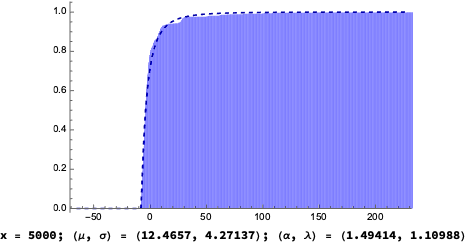
\includegraphics[width=\textwidth]{images/FigureHistogramFit1_v3-GInvFunctionSequenceCalculations.png}}
\end{subfigure}\hfil
\centering
\begin{subfigure}{0.47\textwidth}
\fbox{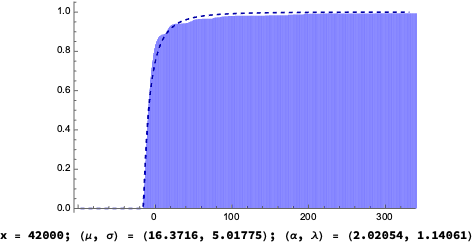
\includegraphics[width=\textwidth]{images/FigureHistogramFit2_v3-GInvFunctionSequenceCalculations.png}}
\end{subfigure}
\end{subfigure}

\captionsetup{justification=centering}
\caption{Numerical computation of the conjectured distribution of $|g(n)|$ in 
	 Proposition \hlocalref{cor_CLT_VII} 
	 for a special case.} 
\label{figure_HistgInvnDistUns_Comparisons_v1}

\end{figure}

\begin{remark}
For $x \geq 3$ and $z \in (-\infty, +\infty)$, let the parameterized distribution 
on the left-hand-side of Proposition \hlocalref{cor_CLT_VII} be defined by 
\[
\mathcal{D}_{\Omega}\left(\mu_{\Omega}, \sigma_{\Omega}; x, z\right) := 
     \frac{1}{x} \times \#\left\{3 \leq n \leq x: 
     \sigma_{\Omega}^{-1}(x) \left(|g(n)| - \frac{1}{n} \times \sum_{k \leq n} |g(k)| - 
     \frac{6\mu_{\Omega}(x)}{\pi^2}\right) \leq z\right\}. 
\]
For the special cases of the functions $\mu_{\Omega}(x) := (\log x)\sqrt{\log\log x}$ and 
$\sigma_{\Omega}(x) := \sqrt{(\log x) (\log\log x)}$, the numerical plots in 
Figure \hlocalref{figure_HistgInvnDistUns_Comparisons_v1} 
show numerical computations of the CDF of the histogram distribution of 
$\mathcal{D}_{\Omega}\left(\mu_{\Omega}, \sigma_{\Omega}; x, z\right)$ when 
$x := 5000$ and $x := 42000$. 
The dashed lines in each plot provide an approximate fit by the CDF 
of a shifted log-normal distribution with mean $\alpha$ and standard deviation $\lambda$. 
We observe that similar features in these two histogram distributions appear even for these 
comparitively small $x$. 
\end{remark}

\section{Proofs of the new exact formulas for $M(x)$} 
\label{Section_KeyApplications} 
\label{Section_KeyApplications_NewExactFormulasForMx_FullSectionLabel} 

In this section, we prove the formulas for $M(x)$ involving the partial sums 
of the function $g(n)$ stated in 
Theorem \hlocalref{prop_Mx_SBP_IntegralFormula}. 
These new formulas exactly identify the Mertens function with partial sums of 
positive unsigned arithmetic functions which are sign-weighted by $\lambda(n)$. 
Since the formulas in equations 
\eqref{prop_Mx_SBP_IntegralFormula_PartB} and 
\eqref{eqn_RmkInitialConnectionOfMxToGInvx_ProvedByInversion_v1} 
suggest that a more complete understanding of the 
asymptotics of the summatory function of $g(n)$ may yield insights into the behavior of 
$M(x)$, we take the time to explore its properties somewhat here as well. 

\subsection{Formulas relating $M(x)$ to the summatory function $G(x)$} 
\label{subSection_KeyApplications_NewExactFormulasForMx} 

\begin{definition}
For any $x \geq 1$, let the partial sums of the Dirichlet convolution $r \ast h$ be defined by 
\begin{align*} 
S_{r \ast h}(x) & := \sum_{n \leq x} \sum_{d|n} r(d) h\left(\frac{n}{d}\right). 
\end{align*}
\end{definition}

\begin{theorem} 
\label{theorem_SummatoryFuncsOfDirCvls} 
Let $r,h: \mathbb{Z}^{+} \rightarrow \mathbb{C}$ be any arithmetic functions such that $r(1) \neq 0$. 
Suppose that $R(x) := \sum_{n \leq x} r(n)$ and $H(x) := \sum_{n \leq x} h(n)$ denote the summatory 
functions of $r$ and $h$, respectively, and that 
$R^{-1}(x) := \sum_{n \leq x} r^{-1}(n)$ for $x \geq 1$. 
The following holds for all integers $x \geq 1$: 
\begin{align*} 
S_{r \ast h}(x) & \phantom{:}= \sum_{d=1}^x r(d) H\left(\Floor{x}{d}\right) \\ 
S_{r \ast h}(x) & \phantom{:}= \sum_{k=1}^{x} H(k) \left(R\left(\Floor{x}{k}\right) - 
     R\left(\Floor{x}{k+1}\right)\right). 
\end{align*} 
Moreover, for any $x \geq 1$ 
\begin{align*} 
H(x) & = \sum_{j=1}^{x} S_{r \ast h}(j) \left(R^{-1}\left(\Floor{x}{j}\right) - 
     R^{-1}\left(\Floor{x}{j+1}\right)\right) \\ 
     & = \sum_{k=1}^{x} r^{-1}(k) S_{r \ast h}(x). 
\end{align*} 
\end{theorem} 

A key consequence of Theorem \hlocalref{theorem_SummatoryFuncsOfDirCvls} 
(proved in the appendix) 
in the special cases where $h(n) := \mu(n)$ for all $n \geq 1$ 
is stated as the next corollary. 

\begin{cor} 
\label{cor_CvlGAstMu} 
Suppose that $r$ is an arithmetic function such that 
$r(1) \neq 0$. Let the summatory function 
$\widetilde{R}(x) := \sum_{n \leq x} (r \ast \mu)(n)$. 
The Mertens function is expressed by the partial sums 
\[
M(x) = \sum_{k=1}^{x} \left(\sum_{j=\floor{\frac{x}{k+1}}+1}^{\floor{\frac{x}{k}}} r^{-1}(j)\right) 
     \widetilde{R}(k), \text{ for } x \geq 1. 
\]
\end{cor} 

\begin{figure}[ht!]

\captionsetup{singlelinecheck=off}
\centering

\begin{subfigure}[t]{0.8\textwidth}
\fbox{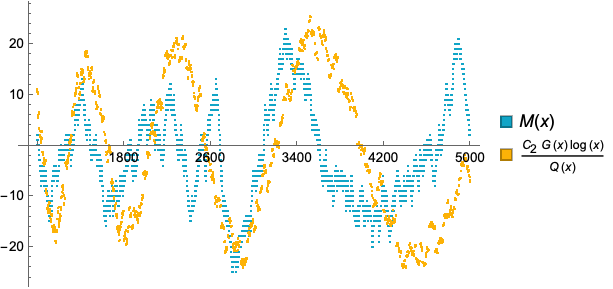
\includegraphics[width=\textwidth]{images/Figure3-CompBetweenMxAndGInvx-GInvFunctionSequenceCalculations.png}}
\end{subfigure}

\captionsetup{justification=centering}
\caption{} 
\label{figure_MxAndNewAuxPartialSums_Comparison_Intro_v2_v1} 

\end{figure} 

\begin{figure}[ht!]

\captionsetup{singlelinecheck=off}
\centering

\begin{subfigure}[t]{0.8\textwidth}
\fbox{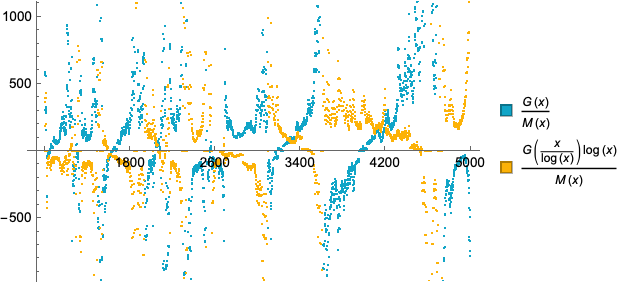
\includegraphics[width=\textwidth]{images/Figure6-RatiosOfGInvToMxAndScaledVersions-GInvFunctionSequenceCalculations.png}}
\captionsetup{justification=centering}
\caption{}
\end{subfigure}

\medskip

\begin{subfigure}[t]{0.8\textwidth}
\fbox{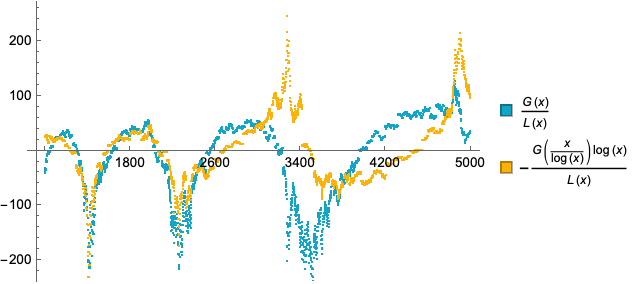
\includegraphics[width=\textwidth]{images/Figure7-RatiosOfGInvToLxAndScaledVersions-GInvFunctionSequenceCalculations.png}}
\captionsetup{justification=centering}
\caption{}
\end{subfigure}

\captionsetup{justification=centering}
\caption{} 
\label{figure_MxLxAndGInvx_Comparison_Intro_v2_v1} 

\end{figure} 

\begin{figure}[ht!]

\captionsetup{singlelinecheck=off}
\centering

\begin{subfigure}[t!]{0.8\textwidth}
\fbox{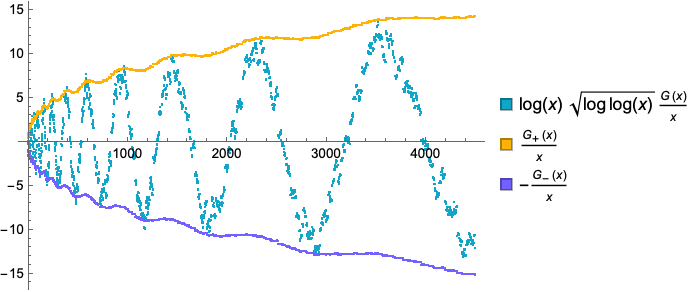
\includegraphics[width=\textwidth]{images/Figure4-ComponentsOfGInvx-GInvFunctionSequenceCalculations.png}}
\captionsetup{justification=centering}
\caption{}
\end{subfigure}

\medskip

\begin{subfigure}[t!]{0.8\textwidth}
\fbox{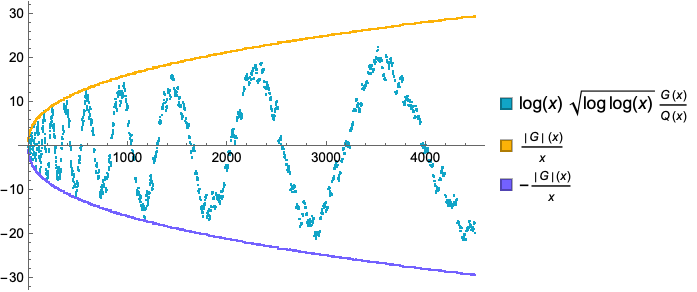
\includegraphics[width=\textwidth]{images/Figure5-ScaledGInvWithBddEnvelopes-GInvFunctionSequenceCalculations.png}}
\captionsetup{justification=centering}
\caption{}
\end{subfigure}

\captionsetup{justification=centering}
\caption{}
\label{figure_MxAndNewAuxPartialSums_Comparison_Intro_v2_v2} 

\end{figure} 

\begin{figure}[ht!]

\captionsetup{singlelinecheck=off}

\begin{subfigure}{\textwidth}
\centering
\begin{subfigure}{0.47\textwidth}
\fbox{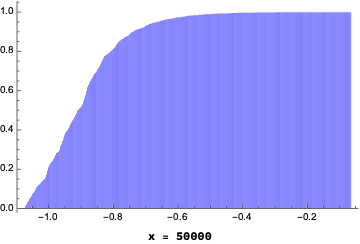
\includegraphics[width=\textwidth]{images/FigureHistogramFit1_GnOvern_v2-GInvFunctionSequenceCalculations.png}}
\end{subfigure}\hfil
\centering
\begin{subfigure}{0.47\textwidth}
\fbox{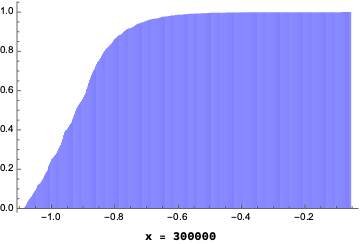
\includegraphics[width=\textwidth]{images/FigureHistogramFit2_GnOvern_v2-GInvFunctionSequenceCalculations.png}}
\end{subfigure}
\captionsetup{justification=centering}
\caption{}
\end{subfigure}

\bigskip

\begin{subfigure}{\textwidth}
\centering
\begin{subfigure}{0.47\textwidth}
\fbox{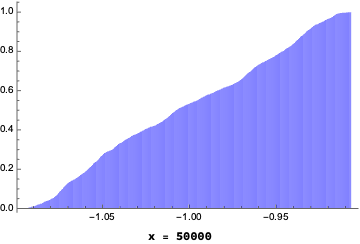
\includegraphics[width=\textwidth]{images/FigureHistogramFit1_GnOvern_v1-GInvFunctionSequenceCalculations.png}}
\end{subfigure}\hfil
\centering
\begin{subfigure}{0.47\textwidth}
\fbox{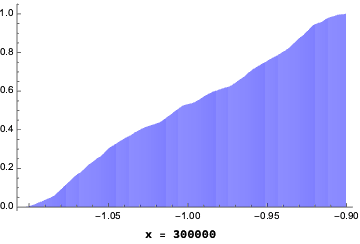
\includegraphics[width=\textwidth]{images/FigureHistogramFit2_GnOvern_v1-GInvFunctionSequenceCalculations.png}}
\end{subfigure}
\captionsetup{justification=centering}
\caption{}
\end{subfigure}

\captionsetup{justification=centering}
\caption{}
\label{figure_HistgInvnDistUns_Comparisons_v2}

\end{figure}

\begin{figure}[ht!]

\captionsetup{singlelinecheck=off}

\begin{subfigure}{\textwidth}
\centering
\begin{subfigure}{0.375\textwidth}
\fbox{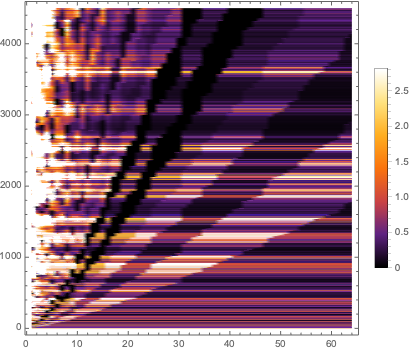
\includegraphics[width=\textwidth]{images/Figure8-GInvPrimemMxAbs.png}}
\end{subfigure}\hfil
\centering
\begin{subfigure}{0.375\textwidth}
\fbox{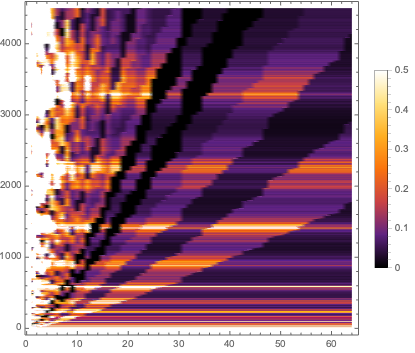
\includegraphics[width=\textwidth]{images/Figure8-GInvPrimemLxAbs.png}}
\end{subfigure}
\captionsetup{justification=centering}
	\caption{$|G[p_m][M](m, x)|$ (left) and $|G[p_m][L](m, x)|$ (right) } 
\end{subfigure}

\smallskip

\begin{subfigure}{\textwidth}
\centering
\begin{subfigure}{0.375\textwidth}
\fbox{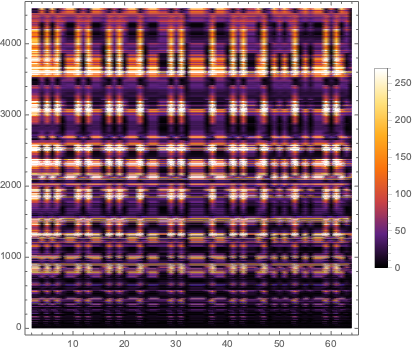
\includegraphics[width=\textwidth]{images/Figure8-GInvBigOmegamMxAbs.png}}
\end{subfigure}\hfil
\centering
\begin{subfigure}{0.375\textwidth}
\fbox{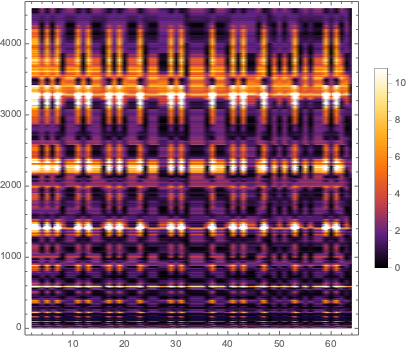
\includegraphics[width=\textwidth]{images/Figure8-GInvBigOmegamLxAbs.png}}
\end{subfigure}
\captionsetup{justification=centering}
\caption{$|G[\Omega][M](m, x)|$ (left) and $|G[\Omega][L](m, x)|$ (right)} 
\end{subfigure}

\smallskip

\begin{subfigure}{\textwidth}
\centering
\begin{subfigure}{0.375\textwidth}
\fbox{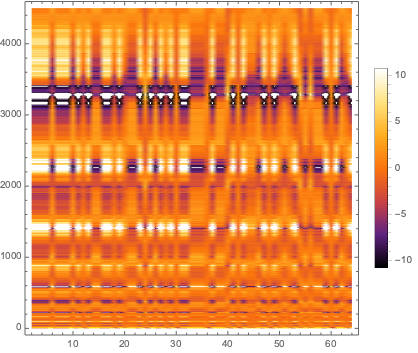
\includegraphics[width=\textwidth]{images/Figure8-GInvCOmegamLxUns.png}}
\end{subfigure}\hfil
\centering
\begin{subfigure}{0.375\textwidth}
\fbox{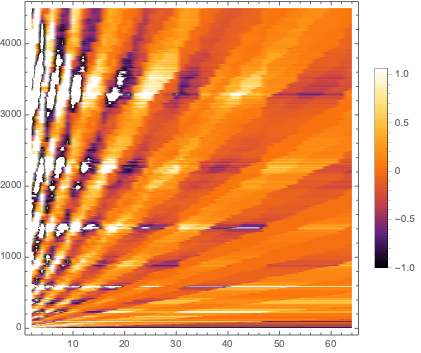
\includegraphics[width=\textwidth]{images/Figure8-GInvPrimeOverLogPrimemLxUns.png}}
\end{subfigure}
\captionsetup{justification=centering}
\caption{$G[C_{\Omega}][L](m, x)$ (left) and $G\left[\frac{p_m}{\log p_m}\right][L](m, x)$ (right)} 
\end{subfigure}

\captionsetup{justification=centering}
\caption{}
\label{figure_LogarithmicRatioDensityPlot_Comparisons_v1}

\end{figure}

\begin{definition}
\label{def_GInvAndGInvAbs_SummFuncs_v2}
\begin{subequations}
The summatory function of $g(n)$ is defined for all $x \geq 1$ by the partial sums 
\begin{equation}
G(x) := \sum_{n \leq x} g(n) = \sum_{n \leq x} \lambda(n) |g(n)|. 
\end{equation}
Let the unsigned partial sums be defined for $x \geq 1$ by 
\begin{equation}
\label{eqn_SummatoryFuncOfUnsignedInverseSeq_v1} 
|G|(x) := \sum_{n \leq x} |g(n)|. 
\end{equation}
\end{subequations}
\end{definition}

Based on the convolution identity in \eqref{eqn_AntiqueDivisorSumIdent}, 
we prove the formulas in 
Theorem \hlocalref{prop_Mx_SBP_IntegralFormula} as special cases of 
Corollary \hlocalref{cor_CvlGAstMu}. 
 
\begin{proof}[Proof of 
              \eqref{prop_Mx_SBP_IntegralFormula_PartA} and \eqref{prop_Mx_SBP_IntegralFormula_PartB} in 
              Theorem \hlocalref{prop_Mx_SBP_IntegralFormula}] 
By applying Theorem \hlocalref{theorem_SummatoryFuncsOfDirCvls} to 
equation \eqref{eqn_AntiqueDivisorSumIdent} we have that 
\begin{align} 
\notag
M(x) & = \sum_{k=1}^{x} \left(\pi\left(\Floor{x}{k}\right)+1\right) g(k) \\ 
\notag 
     & = G(x) + \sum_{k=1}^{\frac{x}{2}} \pi\left(\Floor{x}{k}\right) g(k) \\ 
\notag 
     & = G(x) + G\left(\Floor{x}{2}\right) + 
     \sum_{k=1}^{\frac{x}{2}-1} \left( 
     \pi\left(\Floor{x}{k}\right) - \pi\left(\Floor{x}{k+1}\right) 
	\right) G(k).
\end{align} 
The upper bound on the sum is truncated to $k \in \left[1, \frac{x}{2}\right]$ in the second equation 
above because $\pi(1) = 0$. 
The third formula above follows directly by summation by parts. 
\end{proof} 
\begin{proof}[Proof of \eqref{eqn_RmkInitialConnectionOfMxToGInvx_ProvedByInversion_v1} in Theorem \hlocalref{prop_Mx_SBP_IntegralFormula}]
Lemma \hlocalref{lemma_AnExactFormulaFor_gInvByMobiusInv_v1} shows that 
\[
G(x) = \sum_{d \leq x} \lambda(d) C_{\Omega}(d) M\left(\Floor{x}{d}\right). 
\]
The identity in \eqref{eqn_AntiqueDivisorSumIdent} implies 
$$\lambda(d) C_{\Omega}(d) = (g \ast 1)(d) = (\chi_{\mathbb{P}} + \varepsilon)^{-1}(d).$$ 
We recover the stated result by classical inversion of summatory functions. 
\end{proof}

\subsection{Plots and numerical experiments}

Bounds on the partial sums over the unsigned inverse function in 
\eqref{eqn_SummatoryFuncOfUnsignedInverseSeq_v1} 
contain local information about $G(x)$ through its connection to $|G|(x)$ whose asymptotic 
behavior is given by the average order formula in 
Theorem \hlocalref{cor_ExpectationFormulaAbsgInvn_v2}. 
The plots shown in the figures in this section compare 
the values of $M(x)$, $L(x)$ and $G(x)$ with scaled forms of related auxilliary partial sums: 
\begin{itemize}[noitemsep,topsep=0pt,leftmargin=0.23in]

\item In Figure \hlocalref{figure_MxAndNewAuxPartialSums_Comparison_Intro_v2_v1} 
      we plot a comparison of $M(x)$ and a scaled form of $G(x)$ for $x \leq 5000$ where 
      the absolute constant $C_2 := \zeta(2)$ and where the function 
      $Q(x) := \sum_{n \leq x} \mu^2(n)$ counts the number of squarefree integers $n \leq x$ for any 
      $x \geq 1$. A shift to the left on the $x$-axis of the former function 
      is compared and seen to be similar in shape to the magnitude of $M(x)$ on this initial subinterval. 

\item In Figure \hlocalref{figure_MxLxAndGInvx_Comparison_Intro_v2_v1} we provide the oscillatory 
      ratios of $G(x)$ to $M(x)$ and $L(x)$, respectively, for $x \leq 5000$. 
      In constructing these plots, the ratios displayed are taken to be zero when the denominator 
      summatory function is zero-valued. 
      The plots in (a) exhibit reflected and rotated symmetry within 
      clearly visible subintervals of the plot.
      The plots in (b) are viewed to compare the signed magnitudes of local extremum 
      on subintervals. 

\item In Figure \hlocalref{figure_MxAndNewAuxPartialSums_Comparison_Intro_v2_v2} we compare 
      envelopes on the logarithmically scaled values of $\frac{G(x)}{x}$ to other variants of 
      the partial sums of $g(n)$ for $x \leq 4500$. 
      In (a) we define $G(x) := G_{+}(x) - G_{-}(x)$ where the functions 
      $G_{+}(x) > 0$ and $G_{-}(x) > 0$ for all $x \geq 1$ 
      so that these signed component functions denote the unsigned contributions of only those summands 
      $|g(n)|$ over $n \leq x$ such that $\lambda(n) = \pm 1$, respectively. 
      The summatory function $Q(x)$ in (b) has the same definition as above. 
      By Theorem \hlocalref{cor_ExpectationFormulaAbsgInvn_v2}, 
      \[
      \frac{|G|(x)}{x} \sim \frac{6B_0}{\pi^2} (\log x) \sqrt{\log\log x}, 
      \]
      whereas $|G(x)| \leq |G|(x)$ for all $x \geq 1$ so that we have 
      \[
      \frac{|G(x)| (\log x) \sqrt{\log\log x}}{Q(x)} \ll (\log x)^2 (\log\log x). 
      \]
      Thus, the bounding envelopes on $G(x)$ plotted in (b) may actually hold for all sufficiently 
      large $x$ as the scaling factor is only a logarithmic function of $x$ away from the upper bound 
      and since for most $x$ 
      we expect substantial cancellation in the summands of $|G(x)|$ due to the signed weights by 
      $\lambda(n)$. 

\item In Figure \hlocalref{figure_HistgInvnDistUns_Comparisons_v2} we compare two variants of the 
      distribution of $\frac{G(n)}{n}$ for $3 \leq n \leq x$. For large $x \geq 3$ and bounded 
      real $z$, we define 
      \begin{align*}
      \mathcal{G}_1(x, z) & := \frac{1}{x} \times \left\{3 \leq n \leq x: 
           \frac{G(n)n^{-1} - \log n \sqrt{\log\log n}}{\log x \sqrt{\log\log x}} \leq z\right\}, \\ 
      \mathcal{G}_2(x, z) & := \frac{1}{x} \times \left\{3 \leq n \leq x: 
           \frac{G(n)n^{-1} - \log x \sqrt{\log\log x}}{\log x \sqrt{\log\log x}} \leq z\right\}. 
      \end{align*} 
      The normalized histograms in (a) and (b) respectively show the CDFs corresponding to $\mathcal{G}_1(x, z)$ and 
      $\mathcal{G}_2(x, z)$. The scaling the function $G(n)$ by $n^{-1}$ shows key features of these 
      distributions at the specified two values of $x$ with only a small bounded spread of possible values for $z$. 
      The two numerically small $x$ corresponding to the columns of the plots in (a) and (b) 
      each show apparent quick convergence to a limiting distribution with the same shape and local peaks. 
      The right-hand-side function in the numerator differences of each of the two distribution variants is 
      selected for comparison with the scaled average order of $|g(n)|$. 

\item In Figure \hlocalref{figure_LogarithmicRatioDensityPlot_Comparisons_v1} we define 
      \[
      R[f][S](m, x) := R\left(\floor{\frac{x}{f(m)} \log\left(1 + \frac{x}{f(m)}\right)^{-1}}\right) S(x)^{-1}, 
      \]
      where we shift the denominator by positive one whenever $S(x) = 0$. 
      The integer-valued input $2 \leq m \leq 64$ is shown along the horizontal axis with $1 \leq x \leq 4500$ along the 
      vertical axis in the density plots above. 
      The smoother transitions featured in the density plots of (a) and  (b) 
      comparing $L(x)$ to $M(x)$ (right and left) for the same sequence $f$ 
      show that there is more apparent correlation between $G(x)$ and the former function viewed within this context. 
      Experiments with other sequences $f$ are less visually regular than the selections displayed in the figure. 
      Computer simulations with $f(m)$ selected randomly from the interval $[1, m]$ 
      produce chaotic plots (not shown) with no distinctive features nor apparent correlation with the 
      denominator summatory functions in general.

\end{itemize}

\subsection{Local cancellation of 
	    the formulas for $M(x)$ involving $G(x)$ along a subsequence} 
\label{subSection_LocalCancellationOfGInvx} 

We expect that there is usually (almost always) 
a large amount cancellation between the successive 
values of the summatory function in 
\eqref{eqn_RmkInitialConnectionOfMxToGInvx_ProvedByInversion_v1}. 
Proposition \hlocalref{theorem_PrimorialSeqGInvCalcs_v1} 
demonstrates the phenomenon well along the infinite 
subsequence of the primorials $\{(4m+1)\#\}_{m \geq 1}$ 
(see the discussion in 
Remark \hlocalref{remark_LocalCancellationWithGxAlongThePrimorialsUnderTheRH} below).

\begin{definition}
Suppose that $p_n$ denotes the $n^{th}$ prime for $n \geq 1$ 
\cite[\seqnum{A000040}]{OEIS}. 
Let $\mathcal{P}_{\#}$ denote the set of primorial integers given by  
\cite[\seqnum{A002110}]{OEIS} 
\[
\mathcal{P}_{\#} = \left\{n\#\right\}_{n \geq 1} = \left\{\prod_{k=1}^{n} p_k : n \geq 1\right\}. 
\]
\end{definition}

\begin{prop}
\label{theorem_PrimorialSeqGInvCalcs_v1} 
As $m \rightarrow \infty$ each of the following holds: 
\begin{align} 
\tag{A} 
-G((4m+1)\#) & \asymp (4m+1)!, \\ 
\tag{B} 
G\left(\frac{(4m+1)\#}{p_k}\right) & \asymp (4m)!, 
     \text{ for any } 1 \leq k \leq 4m+1. 
\end{align} 
\end{prop}
\begin{proof} 
We have by \eqref{eqn_PropB_lemma_gInv_MxExample} 
that for all squarefree integers $n \geq 1$ 
\begin{align*} 
|g(n)| & = \sum_{j=0}^{\omega(n)} \binom{\omega(n)}{j} \times j! 
     = (\omega(n))! \times \sum_{j=0}^{\omega(n)} \frac{1}{j!} \\ 
     & = (\omega(n))! \times \left(e + O\left(\frac{1}{(\omega(n)+1)!}\right)\right). 
\end{align*} 
Let $m$ be a large positive integer. 
We obtain main terms of the form 
\begin{align} 
\label{eqn_proof_tag_GinvxLocalCancellation_v1} 
\sum_{\substack{n \leq (4m+1)\# \\ \omega(n)=\Omega(n)}} \lambda(n) |g(n)| 
     & = \sum_{0 \leq k \leq 4m+1} \binom{4m+1}{k} (-1)^{k} k! 
     \left(e + O\left(\frac{1}{(k+1)!}\right)\right) \\ 
\notag 
     & = -(4m+1)! + O\left(\frac{1}{4m+1}\right). 
\end{align} 
The formula for $C_{\Omega}(n)$ stated in 
\eqref{eqn_proof_tag_hInvn_ExactNestedSumFormula_CombInterpetIdent_v3} 
then implies the result in (A). 
Namely, this follows since the contributions from the summands of the inner 
summation on the right-hand-side of 
\eqref{eqn_proof_tag_GinvxLocalCancellation_v1} 
off of the squarefree integers 
are at most a bounded multiple of $(-1)^k k!$ when $\Omega(n) = k$. 
We can similarly derive that for any $1 \leq k \leq 4m+1$ 
\begin{align*}
G\left(\frac{(4m+1)\#}{p_k}\right) & \asymp \sum_{0 \leq k \leq 4m} \binom{4m}{k} (-1)^{k} k! 
     \left(e + O\left(\frac{1}{(k+1)!}\right)\right) = (4m)! + O\left(\frac{1}{4m+1}\right). 
     \qedhere 
\end{align*}
\end{proof}

\begin{remark}
\label{remark_LocalCancellationWithGxAlongThePrimorialsUnderTheRH} 
The Riemann hypothesis (RH) is equivalent to showing that 
\begin{equation} 
\label{eqn_MertensMx_RHEquivProblem_Stmt_intro} 
M(x) = O\left(x^{\frac{1}{2}+\epsilon}\right), \text{ for all } 0 < \epsilon < \frac{1}{2}.
\end{equation}
The RH requires that the sums of the leading constants with opposing signs 
on the asymptotic bounds for the functions from the lemma match. 
In particular, we have that 
\cite{DUSART-1999,DUSART-2010} 
\[
n\# \sim e^{\vartheta(p_n)} \asymp n^n (\log n)^n e^{-n(1+o(1))}, 
     \text{ as } n \rightarrow \infty. 
\]
The observation on the necessary cancellation in 
\eqref{eqn_RmkInitialConnectionOfMxToGInvx_ProvedByInversion_v1}
then follows from the fact that if we obtain a contrary result  
\[
\frac{M((4m+1)\#)}{\sqrt{(4m+1)\#}} \gg \left[(4m+1)\#\right]^{\delta_0}, 
     \text{ as } m \rightarrow \infty, 
\]
for some fixed $\delta_0 > 0$ 
(in contradiction to \eqref{eqn_MertensMx_RHEquivProblem_Stmt_intro} above). 
Assuming the RH, the error terms on the sums we obtained in the proof of 
Proposition \hlocalref{theorem_PrimorialSeqGInvCalcs_v1} actually show that 
the values of the Mertens function are absolutely bounded along this subsequence: 
$$M((4m+1)\#) = O(1), \text{ as } m \rightarrow \infty.$$ 
\end{remark}

\section{Conclusions}

We have identified a sequence, 
$\{g(n)\}_{n \geq 1}$, that is the Dirichlet inverse of the 
shifted strongly additive function $\omega(n)$. 
We showed that there is a natural 
combinatorial interpretation to the repetition of distinct values 
of $|g(n)|$ in terms of the configuration of the 
exponents in the prime factorization of any $n \geq 2$. 
The sign of $g(n)$ is given by $\lambda(n)$ for all $n \geq 1$. 
This leads to a new exact relations of the 
summatory function $G(x)$ to $M(x)$ and the classical partial sums $L(x)$. 
In the process of studying the unsigned sequences, 
we have formalized and conjectured a probabilistic perspective from which to express 
our intuition about features of the distribution of $G(x)$ 
via the properties of its $\lambda(n)$-sign-weighted summands.

The new results proved within this article 
are significant in providing a new window through which we can view bounding $M(x)$ 
through asymptotics of the auxiliary unsigned sequences and their partial sums. 
The computational data generated in 
Table \hlocalref{table_conjecture_Mertens_ginvSeq_approx_values} of the appendix section 
is suggests numerically that the distribution of $G(x)$ is easier to work with 
than a direct treatment of $M(x)$ or $L(x)$. 
We expect that the methods behind the proofs we 
provide with respect to the Mertens function case can be generalized to identify 
associated strongly additive functions with the same role of $\omega(n)$ in this article. 
In particular, we expect that such extensions exist in connection with the signed Dirichlet inverse 
of any multiplicative $f > 0$ and its partial sums. 

\section*{Acknowledgments}
\addcontentsline{toc}{section}{Acknowledgments}

We thank the following mathematicians for offering significant 
discussion, feedback and correspondence over the many drafts of this manuscript: 
Gerg\H{o} Nemes, Jeffrey Lagarias, Robert Vaughan, Steven J.~Miller, 
Paul Pollack and Bruce Reznick. 
The work on the article was supported in part by 
funding made available within the School of Mathematics at the 
Georgia Institute of Technology in 2020 and 2021. 
Without this combined support the article would not have been possible.

\renewcommand{\refname}{References} 
\addcontentsline{toc}{section}{References}
%\bibliography{glossaries-bibtex/thesis-references}{}
\bibliographystyle{plain}

\begin{thebibliography}{10}

\bibitem{APOSTOLANUMT}
T.~M. Apostol.
\newblock {\em Introduction to Analytic Number Theory}.
\newblock Springer--Verlag, 1976.

\bibitem{ANT-BATEMAN-DIAMOND}
P.~T. Bateman and H.~G. Diamond.
\newblock {\em Analytic Number Theory}.
\newblock World Scientific Publishing, 2004.

\bibitem{BILLINGSLY-CLT-PRIMEDIVFUNC}
P.~Billingsley.
\newblock On the central limit theorem for the prime divisor function.
\newblock {\em Amer. Math. Monthly}, 76(2):132--139, 1969.

\bibitem{DEHEUVELS198865}
P.~Deheuvels and D.~Pfeifer.
\newblock {P}oisson approximations of multinomial distributions and point
  processes.
\newblock {\em Journal of Multivariate Analysis}, 25(1):65--89, 1988.

\bibitem{DUSART-1999}
P.~Dusart.
\newblock The $k^{th}$ prime is greater than $k(\log k +\log\log k-1)$ for $k
  \geq 2$.
\newblock {\em Math. Comp.}, 68(225):411--415, 1999.

\bibitem{DUSART-2010}
P.~Dusart.
\newblock Estimates of some functions over primes without {R}.{H}, 2010.

\bibitem{ERDOS-KAC-REF}
P.~Erd{\H{o}}s and M.~Kac.
\newblock The {G}aussian errors in the theory of additive arithmetic functions.
\newblock {\em American Journal of Mathematics}, 62(1):738--742, 1940.

\bibitem{MR3779960}
N.~Frantzikinakis and B.~Host.
\newblock The logarithmic {S}arnak conjecture for ergodic weights.
\newblock {\em Ann. of Math. (2)}, 187(3):869--931, 2018.

\bibitem{FROBERG-1968}
C.~E. Fr{\"{o}}berg.
\newblock On the prime zeta function.
\newblock {\em BIT Numerical Mathematics}, 8:87--202, 1968.

\bibitem{MR2877066}
B.~Green and T.~Tao.
\newblock The {M}\"{o}bius function is strongly orthogonal to nilsequences.
\newblock {\em Ann. of Math. (2)}, 175(2):541--566, 2012.

\bibitem{HARDYWRIGHT}
G.~H. Hardy and E.~M. Wright, editors.
\newblock {\em An Introduction to the Theory of Numbers}.
\newblock Oxford University Press, 2008 (Sixth Edition).

\bibitem{HUMPHRIES-JNT-2013}
P.~Humphries.
\newblock The distribution of weighted sums of the {L}iouville function and
  {P}\'{o}lya's conjecture.
\newblock {\em J. Number Theory}, 133:545--582, 2013.

\bibitem{CLT-RANDOM-ORDERED-FACTS-2011}
H.~Hwang and S.~Janson.
\newblock A central limit theorem for random ordered factorizations of
  integers.
\newblock {\em Electron. J. Probab.}, 16(12):347--361, 2011.

\bibitem{LEHMAN-1960}
R.~S. Lehman.
\newblock On {L}iouville's function.
\newblock {\em Math. Comput.}, 14:311--320, 1960.

\bibitem{MV}
H.~L. Montgomery and R.~C. Vaughan.
\newblock {\em Multiplicative Number Theory: I. Classical Theory}.
\newblock Cambridge, 2006.

\bibitem{NEMES2015C}
G.~Nemes.
\newblock The resurgence properties of the incomplete gamma function {II}.
\newblock {\em Stud. Appl. Math.}, 135(1):86--116, 2015.

\bibitem{NEMES2016}
G.~Nemes.
\newblock The resurgence properties of the incomplete gamma function {I}.
\newblock {\em Anal. Appl. (Singap.)}, 14(5):631--677, 2016.

\bibitem{NEMES2019}
G.~Nemes and A.~B.~Olde Daalhuis.
\newblock Asymptotic expansions for the incomplete gamma function in the
  transition regions.
\newblock {\em Math. Comp.}, 88(318):1805--1827, 2019.

\bibitem{NISTHB}
F.~W.~J. Olver, D.~W. Lozier, R.~F. Boisvert, and C.~W. Clark, editors.
\newblock {\em {NIST} Handbook of Mathematical Functions}.
\newblock Cambridge University Press, 2010.

\bibitem{LOG-COMB-STRUCTS-BOOK}
A.~D.~Barbour R.~Arratia and Simon Tavar{\'{e}}.
\newblock {\em Logarithmic Combinatorial Structures: A Probabilistic Approach}.
\newblock Preprint draft, 2002.

\bibitem{SELBERG-NOTE-SATHE}
A.~Selberg.
\newblock Note on a paper by {L}. {G}. {S}athe.
\newblock {\em J. {I}ndian Math. Soc.}, 18(1):83--87, 1954.

\bibitem{OEIS}
N.~J.~A. Sloane.
\newblock The {O}nline {E}ncyclopedia of {I}nteger {S}equences, 2021.
\newblock \url{http://oeis.org}.

\bibitem{TENENBAUM-PROBNUMT-METHODS}
G.~Tenenbaum.
\newblock {\em Introduction to Analytic and Probabilistic Number Theory}.
\newblock American Mathematical Society, third edition, 2015.

\bibitem{LUNE-DRESSLER}
J.~van~de Lune and R.~E. Dressler.
\newblock Some theorems concerning the number theoretic function $\omega(n)$.
\newblock {\em J. Reine Angew. Math.}, 1975(277):117--119, 1975.

\end{thebibliography}

\bigskip\hrule\smallskip 

\appendix
\cftaddtitleline{toc}{section}{Appendices on supplementary material}{}
\setcounter{section}{0} 
\renewcommand{\thesection}{\Alph{section}} 

%\newpage
\section{Glossary of notation and conventions}
\label{Section_NotationAndConventions}

The next listing provides a 
glossary of common notation, conventions and 
abbreviations used in the article. 

\renewcommand*{\glsclearpage}{}
\renewcommand{\glossarysection}[2][]{}
\printglossary[type={symbols},
               style={glossstyleSymbol},
               nogroupskip=true]

%\section{The Mertens function}
%\label{subSection_Intro_Mx_properties} 
%
%An approach to evaluating the 
%behavior of $M(x)$ for large $x \rightarrow \infty$ considers an 
%inverse Mellin transform of the reciprocal of the Riemann zeta function given by 
%\[
%\frac{1}{\zeta(s)} = \prod_{p} \left(1 - \frac{1}{p^s}\right) = 
%     s \times \int_1^{\infty} \frac{M(x)}{x^{s+1}} dx, \text{ for } \Re(s) > 1. 
%\]
%%We then obtain the following contour integral representation of $M(x)$ for $x \geq 1$: 
%%\[
%%M(x) = \lim_{T \rightarrow \infty}\ \frac{1}{2\pi\imath} \times \int_{T-\imath\infty}^{T+\imath\infty} 
%%     \frac{x^s}{s \zeta(s)} ds. 
%%\] 
%The previous formulas lead to the 
%exact expression of $M(x)$ for any $x > 0$ in the next theorem. 
%\nocite{TITCHMARSH} 
%
%\begin{theorem}[Titchmarsh] 
%\label{theorem_MxMellinTransformInvFormula} 
%Assuming the Riemann Hypothesis (RH), there exists an infinite sequence 
%$\{T_k\}_{k \geq 1}$ satisfying $k \leq T_k \leq k+1$ for each integer $k \geq 1$ 
%such that for any $x > 0$ 
%\[
%M(x) = \lim_{k \rightarrow \infty} 
%     \sum_{\substack{\rho: \zeta(\rho) = 0 \\ 0 < |\Im(\rho)| < T_k}} 
%     \frac{x^{\rho}}{\rho \zeta^{\prime}(\rho)} + 
%     \sum_{n \geq 1} \frac{(-1)^{n-1}}{n (2n)! \zeta(2n+1)} 
%     \left(\frac{2\pi}{x}\right)^{2n} + 
%     \frac{\mu(x)}{2} \Iverson{x \in \mathbb{Z}^{+}} - 2. 
%\] 
%\end{theorem} 
%
%An unconditional bound on the Mertens function due to Walfisz (circa 1963) 
%states that there is an absolute constant $C_1 > 0$ such that 
%$$M(x) \ll x \times \exp\left(-C_1 \log^{\frac{3}{5}}(x) 
%  (\log\log x)^{-\frac{1}{5}}\right).$$ 
%Under the assumption of the RH, Soundararajan and Humphries, respectively, 
%improved estimates bounding $M(x)$ from above for large $x$ in the 
%following forms 
%\cite{SOUND-MERTENS-ANNALS,HUMPHRIES-JNT-2013}: 
%\begin{align*} 
%M(x) & \ll \sqrt{x} \times \exp\left(\sqrt{\log x} (\log\log x)^{14}\right), \\ 
%M(x) & \ll \sqrt{x} \times \exp\left( 
%     \sqrt{\log x} (\log\log x)^{\frac{5}{2}+\epsilon}\right), 
%     \text{ for all } \epsilon > 0. 
%\end{align*} 
%The RH is equivalent to showing that 
%\begin{equation*} 
%M(x) = O\left(x^{\frac{1}{2}+\epsilon}\right), \text{ for all } 0 < \epsilon < \frac{1}{2}.
%\end{equation*}
%There is a rich history to the original statement of the \emph{Mertens conjecture} which 
%asserts that $|M(x)| < C_2 \sqrt{x}$ for an absolute constant $C_2 > 0$. 
%The conjecture was first verified by F.~Mertens himself for $C_2 = 1$ at all $x < 10^{4}$ 
%without the benefit of modern computation. 
%Since its beginnings in 1897, the Mertens conjecture was disproved by computational methods involving 
%non-trivial simple zeta function zeros with comparatively small imaginary parts in the 
%famous paper by Odlyzko and te Riele \cite{ODLYZ-TRIELE}. 
%
%More recent attempts 
%at bounding $M(x)$ naturally consider determining the rates at which the scaled function 
%$M(x) x^{-\frac{1}{2}}$ grows with or without bound along infinite subsequences. 
%It is verified by computation that \cite[\cf \S 4.1]{PRIMEREC} 
%\cite[\cf \seqnum{A051400}; \seqnum{A051401}]{OEIS} 
%\[
%\overline{L} := \limsup_{x\rightarrow\infty} \frac{M(x)}{\sqrt{x}} > 1.060\ 
%     \qquad (\text{more recently } \overline{L} \geq 1.826054), 
%\] 
%and 
%\[ 
%\underline{L} := \liminf_{x\rightarrow\infty} \frac{M(x)}{\sqrt{x}} < -1.009\ 
%     \qquad (\text{more recently } \underline{L} \leq -1.837625). 
%\] 
%Based on the work by Odlyzko and te Riele (circa 1985), it is widely believed that 
%these limiting bounds evaluate to $\pm \infty$, respectively 
%\cite{ODLYZ-TRIELE,MREVISITED,ORDER-MERTENSFN,HURST-2017}. 
%A conjecture due to Gonek asserts that 
%in fact $M(x)$ satisfies \cite{NG-MERTENS}
%$$\limsup_{x \rightarrow \infty} \frac{|M(x)|}{\sqrt{x} (\log\log\log x)^{\frac{5}{4}}} = C_3,$$ 
%for $C_3 > 0$ an absolute constant. 

\section{The distributions of $\omega(n)$ and $\Omega(n)$} 
\label{subSection_TheKnownDistsOfThePrimeOmegaFunctions_IntroResults_v1} 

The next theorems reproduced from \cite[\S 7.4]{MV} bound the frequency of the 
number of $\omega(n)$ and $\Omega(n)$ over $n \leq x$ such that 
$\omega(n),\Omega(n) < \log\log x$ and $\omega(n),\Omega(n) > \log\log x$. 
Since $\frac{1}{n} \times \sum_{k \leq n} \omega(k) = \log\log n + B_1 + o(1)$ and 
$\frac{1}{n} \times \sum_{k \leq n} \Omega(k) = \log\log n + B_2 + o(1)$ for 
$B_1 \approx 0.261497$ and $B_2 \approx 1.03465$ 
absolute constants in each case \cite[\S 22.10]{HARDYWRIGHT}, 
there is a distinctive tendency 
of these strongly additive arithmetic functions towards their respective average orders 
(\cf \cite{ERDOS-KAC-REF,BILLINGSLY-CLT-PRIMEDIVFUNC} \cite[\S 7.4]{MV}). 

\begin{theorem} 
\label{theorem_MV_Thm7.20-init_stmt} 
For $x \geq 2$ and $r > 0$, let 
\begin{align*} 
A(x, r) & := \#\left\{n \leq x: \Omega(n) \leq r \log\log x\right\}, \\ 
B(x, r) & := \#\left\{n \leq x: \Omega(n) \geq r \log\log x\right\}. 
\end{align*} 
If $0 < r \leq 1$, then 
\[
A(x, r) \ll\phantom{_R} x (\log x)^{r-1 - r\log r}, \text{ as } x \rightarrow \infty. 
\]
If $1 \leq r \leq R < 2$, then 
\[
B(x, r) \ll_R x (\log x)^{r-1-r \log r}, \text{ as } x \rightarrow \infty. 
\]
\end{theorem} 

%Theorem \hlocalref{theorem_MV_Thm7.21-init_stmt} is a special case analog of the 
%Erd\H{o}s-Kac theorem for the normally distributed values of 
%$\frac{\omega(n) - \log\log n}{\sqrt{\log\log n}}$ over $n \leq x$ as 
%$x \rightarrow \infty$ \cite[\cf Thm.\ 7.21]{MV} \cite[\cf \S 1.7]{IWANIEC-KOWALSKI}. 
%\begin{theorem}
%\label{theorem_MV_Thm7.21-init_stmt} 
%We have that as $x \rightarrow \infty$ 
%\[
%\#\left\{3 \leq n \leq x: \Omega(n) \leq \log\log n \right\} = 
%     \frac{x}{2} + O\left(\frac{x}{\sqrt{\log\log x}}\right). 
%\]
%\end{theorem} 

\begin{theorem}
\label{theorem_HatPi_ExtInTermsOfGz} 
For integers $k \geq 1$ and $x \geq 2$ 
$$\widehat{\pi}_k(x) := \#\{2 \leq n \leq x: \Omega(n)=k\}.$$ 
For $0 < R < 2$, uniformly for $1 \leq k \leq R \log\log x$ 
\[
\widehat{\pi}_k(x) = \frac{x}{\log x} \times \mathcal{G}\left(\frac{k-1}{\log\log x}\right) 
     \frac{(\log\log x)^{k-1}}{(k-1)!} \left(1 + O_R\left(\frac{k}{(\log\log x)^2}\right)\right), 
\]
where 
\[
\mathcal{G}(z) := \frac{1}{\Gamma(1+z)} \times 
	\prod_p \left(1-\frac{z}{p}\right)^{-1} \left(1-\frac{1}{p}\right)^z, 
	\text{ for } 0 \leq |z| < R. 
\]
\end{theorem} 

\begin{remark} 
\label{remark_MV_Pikx_FuncResultsAnnotated_v1} 
We can extend the work in \cite{MV} on the distribution of $\Omega(n)$ to obtain 
corresponding analogous results for the distribution of $\omega(n)$. 
For $0 < R < 2$ and as $x \rightarrow \infty$ 
\begin{equation}
\label{eqn_Pikx_UniformAsymptoticsStmt_from_MV_v2} 
\pi_k(x) = \frac{x}{\log x} \times 
     \widetilde{\mathcal{G}}\left(\frac{k-1}{\log\log x}\right) 
     \frac{(\log\log x)^{k-1}}{(k-1)!} \left( 
     1 + O_R\left(\frac{k}{(\log\log x)^2}\right) 
     \right), 
\end{equation}
uniformly for $1 \leq k \leq R\log\log x$. 
The factors of the function $\widetilde{\mathcal{G}}(z)$ are 
defined by $\widetilde{\mathcal{G}}(z) := \widetilde{F}(1, z) \times \Gamma(1+z)^{-1}$ where 
\[
\widetilde{F}(s, z) := \prod_p \left(1 + \frac{z}{p^s-1}\right) \left(1 - \frac{1}{p^s}\right)^{z}, 
	\text{ for } \Re(s) > \frac{1}{2} \text{ and } |z| \leq R < 2. 
\]
Let the functions 
\begin{align*} 
C(x, r) & := \#\{n \leq x: \omega(n) \leq r \log\log x\}, \\ 
D(x, r) & := \#\{n \leq x: \omega(n) \geq r \log\log x\}. 
\end{align*} 
The following upper bounds hold as $x \rightarrow \infty$: 
\begin{align*} 
C(x, r) & \ll\phantom{_R} x (\log x)^{r - 1 - r \log r}, \text{ uniformly for } 0 < r \leq 1, \\ 
D(x, r) & \ll_R x (\log x)^{r - 1 - r \log r}, \text{ uniformly for } 1 \leq r \leq R < 2.
\end{align*} 
\end{remark} 

\section{Partial sums expressed in terms of the incomplete gamma function} 
\label{subSection_OtherFactsAndResults} 

We cite the correspondence with Gerg\H{o} Nemes 
from the Alfr\'{e}d R\'{e}nyi Institute of Mathematics and his 
careful notes on the limiting asymptotics for the sums identified in this section. 
The communication of his proofs are adapted to establish the next few lemmas based on 
his work in \cite{NEMES2015C,NEMES2016,NEMES2019}. 

\begin{facts}[The incomplete gamma function] 
\label{facts_ExpIntIncGammaFuncs} 
\begin{subequations}
The (upper) incomplete gamma function is defined by \cite[\S 8.4]{NISTHB} 
\[
\Gamma(a, z) = \int_{z}^{\infty} t^{a-1} e^{-t} dt, \text{ for } 
	a \in \mathbb{R} \text{ and } |\arg z| < \pi.  
\]
The function $\Gamma(a, z)$ can be continued to an analytic function of $z$ on the 
universal covering of $\mathbb{C} \mathbin{\backslash} \{0\}$. 
For $a \in \mathbb{Z}^{+}$, the function $\Gamma(a, z)$ is an entire function of $z$. 
The following properties of $\Gamma(a, z)$ hold \cite[\S 8.4; \S 8.11(i)]{NISTHB}: 
\begin{align} 
\label{eqn_IncompleteGamma_PropA} 
     \Gamma(a, z) & = (a-1)! e^{-z} \times \sum_{k=0}^{a-1} \frac{z^k}{k!}, \text{ for } 
     a \in \mathbb{Z}^{+} \text{ and } z \in \mathbb{C}, \\ 
\label{eqn_IncompleteGamma_PropB} 
\Gamma(a, z) & \sim z^{a-1} e^{-z}, \text{ for fixed } a \in \mathbb{C} 
     \text{ and } z > 0 \text{ as } z \rightarrow +\infty. 
\end{align}
For $z > 0$, as $z \rightarrow +\infty$ we have that \cite{NEMES2015C} 
\begin{equation} 
\label{eqn_IncompleteGamma_PropC}
\Gamma(z, z) = \sqrt{\frac{\pi}{2}} z^{z-\frac{1}{2}} e^{-z} + 
     O\left(z^{z-1} e^{-z}\right), 
\end{equation} 
If $z,a \rightarrow \infty$ with $z = \rho a$ for some $\rho > 1$ such that 
$(\rho - 1)^{-1} = o\left(\sqrt{|a|}\right)$, then \cite{NEMES2015C}
\begin{equation}
\label{eqn_IncompleteGamma_PropD}
\Gamma(a, z) \sim z^a e^{-z} \times \sum_{n \geq 0} \frac{(-a)^n b_n(\rho)}{(z-a)^{2n+1}}. 
\end{equation} 
The sequence $b_n(\rho)$ satisfies $b_0(\rho) = 1$ and 
the recurrence relation 
%\footnote{
%     An exact formula for $b_n(\lambda)$ is given in terms of the 
%     \emph{second-order Eulerian number triangle} 
%     \cite[\seqnum{A008517}]{OEIS} as follows: 
%     \[
%          b_n(\lambda) = \sum_{k=0}^{n} \gkpEII{n}{k} \lambda^{k+1}. 
%     \]
%}
\[
b_n(\rho) = \rho(1-\rho) b_{n-1}^{\prime}(\rho) + \rho(2n-1) b_{n-1}(\rho), 
     \text{ for } n \geq 1. 
\]
\end{subequations}
\end{facts} 

\begin{prop}
\label{prop_IncGammaLambdaTypeBounds_v1}
Let $a,z,\rho$ be positive real parameters such that $z=\rho a$. 
If $\rho \in (0, 1)$, then as $z \rightarrow \infty$ 
\[
\Gamma(a, z) = \Gamma(a) + O_{\rho}\left(z^{a-1} e^{-z}\right). 
\]
If $\rho > 1$, then as 
$z \rightarrow \infty$ 
\[
\Gamma(a, z) = \frac{z^{a-1} e^{-z}}{1-\rho^{-1}} + O_{\rho}\left(z^{a-2} e^{-z}\right). 
\]
If $\rho > W(1) \approx 0.56714$, then as $z \rightarrow \infty$ 
\[
\Gamma(a, z e^{\pm\pi\imath}) = -e^{\pm \pi\imath a} \frac{z^{a-1} e^{z}}{1 + \rho^{-1}} + 
     O_{\rho}\left(z^{a-2} e^{z}\right). 
\]
\end{prop}
The first two estimates are only useful when $\rho$ is bounded away from the 
transition point at one. 
We cannot write the last expansion above 
as $\Gamma(a, -z)$ directly unless $a \in \mathbb{Z}^{+}$ 
as the incomplete gamma function 
has a branch point at the origin with respect to its second variable. 
This function becomes a single-valued 
analytic function of its second input by continuation 
on the universal covering of $\mathbb{C} \mathbin{\backslash} \{0\}$. 
\begin{proof}
The first asymptotic estimate follows directly from the following 
asymptotic series expansion that holds as $z \rightarrow +\infty$ 
\cite[Eq.\ (2.1)]{NEMES2019}: 
\[
\Gamma(a, z) \sim \Gamma(a) + z^a e^{-z} \times \sum_{k \geq 0} 
     \frac{(-a)^k b_k(\rho)}{(z-a)^{2k+1}}. 
\]
Using the notation from \eqref{eqn_IncompleteGamma_PropD} and \cite{NEMES2016} 
\[
\Gamma(a, z) = \frac{z^{a-1} e^{-z}}{1-\rho^{-1}} + z^{a} e^{-z} R_1(a, \rho). 
\]
From the bounds in \cite[\S 3.1]{NEMES2016}, we have 
\[
\left\lvert z^{a} e^{-z} R_1(a, \rho) \right\rvert \leq 
     z^a e^{-z} \times \frac{a \cdot b_1(\rho)}{(z-a)^{3}} = 
     \frac{z^{a-2} e^{-z}}{(1-\rho^{-1})^{3}}
\]
The main and error terms in the previous equation can also be 
seen by applying the asymptotic series in 
\eqref{eqn_IncompleteGamma_PropD} directly. 

The proof of the third equation above follows from the asymptotics 
\cite[Eq.\ (1.1)]{NEMES2015C}
\[
\Gamma(-a, z) \sim z^{-a} e^{-z} \times \sum_{n \geq 0} \frac{a^n b_n(-\rho)}{(z+a)^{2n+1}}, 
\]
by setting $(a, z) \mapsto \left(a e^{\pm \pi\imath}, z e^{\pm \pi\imath}\right)$ so that 
$\rho = \frac{z}{a} > W(1)$. 
The restriction on the range of $\rho$ over which the third formula holds is made to ensure that 
the formula from the reference is valid at negative real $a$. 
\end{proof}

\begin{lemma}
\label{lemma_ConvenientIncGammaFuncTypePartialSumAsymptotics_v2}
As $x \rightarrow +\infty$  
\begin{align*}
\frac{x}{\log x} \times \left\lvert \sum_{1 \leq k \leq \floor{\log\log x}} 
     \frac{(-1)^k (\log\log x)^{k-1}}{(k-1)!} \right\rvert 
     & = \frac{x}{2\sqrt{2\pi \log\log x}} + O\left(\frac{x}{(\log\log x)^{\frac{3}{2}}}\right). 
\end{align*}
\end{lemma}
\begin{proof}
We have for $n \geq 1$ and any $t > 0$ by 
\eqref{eqn_IncompleteGamma_PropA} that 
\[
\sum_{1 \leq k \leq n} \frac{(-1)^k t^{k-1}}{(k-1)!} = -e^{-t} \times 
     \frac{\Gamma(n, -t)}{(n-1)!}. 
\]
Suppose that $t = n + \xi$ with $\xi = O(1)$. 
By the third formula 
in Proposition \hlocalref{prop_IncGammaLambdaTypeBounds_v1} 
with the parameters $(a, z, \lambda) \mapsto \left(n, t, 1 + \frac{\xi}{n}\right)$, 
we deduce that as $n,t \rightarrow +\infty$. 
\begin{equation}
\label{eqn_ProofTag_lemma_ConvenientIncGammaFuncTypePartialSumAsymptotics_v2}
\Gamma(n, -t) = (-1)^{n+1} \times \frac{t^n e^{t}}{t+n} + 
     O\left(\frac{n t^n e^{t}}{(t+n)^3}\right) = 
     (-1)^{n+1} \times \frac{t^n e^t}{2n} + O\left(\frac{t^{n-1} e^t}{n}\right). 
\end{equation}
Accordingly, we see that 
\[
\sum_{1 \leq k \leq n} \frac{(-1)^k t^{k-1}}{(k-1)!} = 
     (-1)^{n} \times \frac{t^n}{2n!} + O\left(\frac{t^{n-1}}{n!}\right). 
\]
By the variant of Stirling's formula in \cite[\cf Eq.\ (5.11.8)]{NISTHB}, we have 
\[
n! = \Gamma(1 + t - \xi) = \sqrt{2\pi} t^{t-\xi+\frac{1}{2}} e^{-t} \left(1 + O\left(t^{-1}\right)\right) = 
     \sqrt{2\pi} t^{n+\frac{1}{2}} e^{-t} \left(1 + O\left(t^{-1}\right)\right). 
\]
Hence, as $n \rightarrow +\infty$ with $t := n + \xi$ and $\xi = O(1)$, we obtain that 
\[
\sum_{k=1}^{n} \frac{(-1)^k t^{k-1}}{(k-1)!} = (-1)^n \times \frac{e^t}{2 \sqrt{2\pi t}} + 
     O\left(e^t t^{-\frac{3}{2}}\right). 
\]
The conclusion follows by taking $n := \floor{\log\log x}$ and $t := \log\log x$. 
\end{proof}

\begin{definition}
For $x \geq 1$, let the summatory function (\cf \cite{LUNE-DRESSLER}) 
\[
L_{\omega}(x) := \sum_{n \leq x} (-1)^{\omega(n)}. 
\]
\end{definition}

\begin{lemma} 
\label{cor_AsymptoticsForSignedSumsOfomegan_v1}
As $x \rightarrow \infty$, there is an absolute constant $A_0 > 0$ such that 
\[
L_{\omega}(x) = 
     \frac{(-1)^{\floor{\log\log x}} x}{A_0 \sqrt{2\pi \log\log x}} + 
     O\left(\frac{x}{\log\log x}\right). 
\]
\end{lemma}
\begin{proof}
An adaptation of the proof of Lemma \hlocalref{lemma_ConvenientIncGammaFuncTypePartialSumAsymptotics_v2} 
provides that for any $a \in (1, 1.76321) \subset \left(1, W(1)^{-1}\right)$ the 
next partial sums satisfy 
\begin{align}
\notag 
\widehat{S}_a(x) & := 
     \frac{x}{\log x} \times \left\lvert \sum_{k=1}^{\floor{a\log\log x}} \frac{(-1)^{k} (\log\log x)^{k-1}}{(k-1)!} 
     \right\rvert \\ 
\label{eqn_ConvenientIncGammaFuncTypePartialSumAsymptotics_va3} 
	& \phantom{:} = \frac{\sqrt{a} x}{\sqrt{2\pi}(a+1) a^{\{a\log\log x\}}} 
     \times \frac{(\log x)^{a-1-a\log a}}{\sqrt{\log\log x}} 
     \left(1 + O\left(\frac{1}{\log\log x}\right)\right). 
\end{align}
Here, we take $\{x\} = x - \floor{x} \in [0, 1)$ to be the fractional part of $x$. 
Suppose that we take $a := \frac{3}{2}$ so that $a-1-a\log a \approx -0.108198$. 
We expand as 
\begin{align*}
L_{\omega}(x) & = 
     \sum_{k \leq \log\log x} 2 (-1)^{k} \pi_k(x) + 
     O\left(\widehat{S}_{\frac{3}{2}}(x) + 
     \#\left\{n \leq x: \omega(n) \geq \frac{3}{2}\log\log x\right\}\right). 
\end{align*} 
The justification for the above error term including $\widehat{S}_{\frac{3}{2}}(x)$ is that for 
$0 \leq z \leq \frac{3}{2}$ we can show that $\widetilde{\mathcal{G}}\left(z\right)$ is bounded. 
We apply the uniform asymptotics for $\pi_k(x)$ that hold as $x \rightarrow \infty$ when 
$1 \leq k \leq R \log\log x$ for $1 \leq R < 2$ from 
Remark \hlocalref{remark_MV_Pikx_FuncResultsAnnotated_v1} to evaluate the sums that provide the 
main term of the expansion in the previous equation. 
We have that $\widetilde{G}(0)=1$ and that for any 
$0 < |z| < 1$ the function $\widetilde{G}(z)$ is positive, monotone in $z$ and 
has an absolutely convergent series expansion in $z$ about zero. 
For integers $m \geq 1$, we see by induction that 
\[
\sum_{k \leq \log\log x} \frac{(-1)^k (k-1)^m (\log\log x)^{k-1-m}}{(k-1)!} = 
     \sum_{k \leq \log\log x} \frac{(-1)^{k+m} (\log\log x)^{k-1}}{(k-1)!} \left( 
     1 + O\left(\frac{1}{\log\log x}\right)\right). 
\]
We then argue 
by Lemma \hlocalref{lemma_ConvenientIncGammaFuncTypePartialSumAsymptotics_v2} 
and \eqref{eqn_ConvenientIncGammaFuncTypePartialSumAsymptotics_va3} 
that for all sufficiently large $x$ 
there is a limiting absolute constant $A_0 > 0$ such that 
\begin{align} 
\label{eqn_cor_AsymptoticsForSignedSumsOfomegan_v1_PfTag_v3} 
L_{\omega}(x) & = \frac{(-1)^{\floor{\log\log x}} x}{A_0 \sqrt{2\pi \log\log x}} + 
     O\left(E_{\omega}(x) + 
     \frac{x}{(\log x)^{0.108198} \sqrt{\log\log x}} + 
     \#\left\{n \leq x: \omega(x) \geq \frac{3}{2}\log\log x\right\}\right). 
\end{align} 
%In fact, we find that 
%\[
%A_0 = \lim_{x \rightarrow \infty} \widetilde{G}\left(1-\frac{1}{\log\log x}\right) = 
%     \widetilde{G}(1) \approx 1. 
%\]
The error term in \eqref{eqn_cor_AsymptoticsForSignedSumsOfomegan_v1_PfTag_v3} 
is bounded as follows when $x \rightarrow \infty$ using Stirling's formula, 
\eqref{eqn_IncompleteGamma_PropA} and 
\eqref{eqn_IncompleteGamma_PropC}:  
\begin{align*} 
E_{\omega}(x) & \ll \frac{x}{\log x} \times 
     \sum_{1 \leq k \leq \log\log x} \frac{(\log\log x)^{k-2}}{(k-1)!} \\ 
     & = 
     \frac{x \Gamma(\log\log x, \log\log x)}{\Gamma(\log\log x + 1)} 
     = \frac{x}{2\log\log x} \left(1 + O\left(\frac{1}{\sqrt{\log\log x}}\right)\right). 
\end{align*}
Finally, by an application of the results in 
Remark \hlocalref{remark_MV_Pikx_FuncResultsAnnotated_v1} 
\[
\#\left\{n \leq x: \omega(x) \geq \frac{3}{2}\log\log x\right\} \ll 
     \frac{x}{(\log x)^{0.108198}}. 
     \qedhere 
\] 
\end{proof}

\section{Inversion theorems for partial sums of Dirichlet convolutions}
\label{Section_PrelimProofs_Config} 
\label{subSection_PrelimProofs_Config_InversionTheorem}

We give a proof of the inversion type results in 
Theorem \hlocalref{theorem_SummatoryFuncsOfDirCvls} 
below by matrix methods. 
Related results on summations of Dirichlet convolutions and their inversion appear in 
\cite[\S 2.14; \S 3.10; \S 3.12; \cf \S 4.9, p.\ 95]{APOSTOLANUMT}. 

\begin{proof}[Proof of Theorem \hlocalref{theorem_SummatoryFuncsOfDirCvls}] 
\label{proofOf_theorem_SummatoryFuncsOfDirCvls} 
Let $h,r$ be arithmetic functions such that $r(1) \neq 0$. 
The following formulas hold for all $x \geq 1$: 
\begin{align} 
\notag 
S_{r \ast h}(x) & := \sum_{n=1}^{x} \sum_{d|n} r(n) h\left(\frac{n}{d}\right) = 
     \sum_{d=1}^x r(d) H\left(\floor{\frac{x}{d}}\right) \\ 
\label{eqn_proof_tag_PigAsthx_ExactSummationFormula_exp_v2} 
     & = \sum_{i=1}^x \left(R\left(\floor{\frac{x}{i}}\right) - R\left(\floor{\frac{x}{i+1}}\right)\right) H(i). 
\end{align} 
The first formula on the right-hand-side above is well known from the references. 
The second formula is justified directly using 
summation by parts as \cite[\S 2.10(ii)]{NISTHB} 
\begin{align*} 
S_{r \ast h}(x) & = \sum_{d=1}^x h(d) R\left(\floor{\frac{x}{d}}\right) \\ 
     & = \sum_{i \leq x} \left(\sum_{j \leq i} h(j)\right) \times 
     \left(R\left(\floor{\frac{x}{i}}\right) - 
     R\left(\floor{\frac{x}{i+1}}\right)\right). 
\end{align*} 
We form the invertible matrix of coefficients, denoted by $\hat{R}$ below, 
associated with the linear system defining $H(j)$ for all 
$1 \leq j \leq x$ in \eqref{eqn_proof_tag_PigAsthx_ExactSummationFormula_exp_v2} by setting 
\[
r_{x,j} := R\left(\floor{\frac{x}{j}}\right) - R\left(\floor{\frac{x}{j+1}}\right) 
     \equiv R_{x,j} - R_{x,j+1}, 
\] 
with 
\[
R_{x,j} := R\left(\Floor{x}{j}\right), \text{ for } 1 \leq j \leq x. 
\]
Since $r_{x,x} = R(1) = r(1) \neq 0$ for all $x \geq 1$ and $r_{x,j} = 0$ for all $j > x$, 
the matrix we have defined in this problem is lower triangular with a non-zero 
constant on its diagonals, and so is invertible. 
If we let $\hat{R} := (R_{x,j})$, then the next matrix is 
expressed by applying an invertible shift operation as 
\[
(r_{x,j}) = \hat{R} \left(I - U^{T}\right). 
\]
The square matrix $U$ of sufficiently large finite dimensions $N \times N$ for $N \geq x$ 
has $(i,j)^{th}$ entries for all $1 \leq i,j \leq N$ that are defined by 
$(U)_{i,j} = \delta_{i+1,j}$ so that 
\[
\left[\left(I - U^T\right)^{-1}\right]_{i,j} = \Iverson{j \leq i}. 
\]
We observe that 
\[
\Floor{x}{j} - \Floor{x-1}{j} = \begin{cases} 
     1, & \text{ if $j|x$; } \\ 
     0, & \text{ otherwise. } 
     \end{cases} 
\] 
The previous equation implies that 
\begin{equation} 
\label{eqn_proof_tag_FloorFuncDiffsOfSummatoryFuncs_v2} 
R\left(\floor{\frac{x}{j}}\right) - R\left(\floor{\frac{x-1}{j}}\right) = 
     \begin{cases} 
     r\left(\frac{x}{j}\right), & \text{ if $j | x$; } \\ 
     0, & \text{ otherwise. } 
     \end{cases}
\end{equation} 
We use the property in \eqref{eqn_proof_tag_FloorFuncDiffsOfSummatoryFuncs_v2} 
to shift the matrix $\hat{R}$, and then invert the result to obtain a matrix involving the 
Dirichlet inverse of $r$ as follows: 
\begin{align*} 
\left(\left(I-U^{T}\right) \hat{R}\right)^{-1} & = 
     \left(r\left(\frac{x}{j}\right) \Iverson{j|x}\right)^{-1} = 
     \left(r^{-1}\left(\frac{x}{j}\right) \Iverson{j|x}\right). 
\end{align*} 
Our target matrix in the inversion problem is defined by 
$$(r_{x,j}) = \left(I-U^{T}\right) \left(r\left(\frac{x}{j}\right) \Iverson{j|x}\right) \left(I-U^{T}\right)^{-1}.$$
We can express its inverse by a similarity transformation conjugated by shift operators in the form of 
\begin{align*} 
(r_{x,j})^{-1} & = \left(I-U^{T}\right)^{-1} \left(r^{-1}\left(\frac{x}{j}\right) 
     \Iverson{j|x}\right) \left(I-U^{T}\right) \\ 
     & = \left(\sum_{k=1}^{\floor{\frac{x}{j}}} r^{-1}(k)\right) \left(I-U^{T}\right) \\ 
     & = \left(\sum_{k=1}^{\floor{\frac{x}{j}}} r^{-1}(k) - \sum_{k=1}^{\floor{\frac{x}{j+1}}} r^{-1}(k)\right). 
\end{align*} 
The summatory function $H(x)$ is given exactly for any integers $x \geq 1$ 
by a vector product with the inverse matrix from the previous equation in the form of 
\begin{align*} 
H(x) & = \sum_{k=1}^x \left(\sum_{j=\floor{\frac{x}{k+1}}+1}^{\floor{\frac{x}{k}}} r^{-1}(j)\right) 
     \times S_{r \ast h}(k). 
\end{align*} 
We can prove a second inversion formula providing the coefficients of the summatory function 
$R^{-1}(j)$ for $1 \leq j \leq x$ from the last equation by adapting our argument to prove 
\eqref{eqn_proof_tag_PigAsthx_ExactSummationFormula_exp_v2} above. 
This leads to the alternate identity expressing $H(x)$ given by 
\[
H(x) = \sum_{k=1}^{x} r^{-1}(k) \times S_{r \ast h}\left(\Floor{x}{k}\right). 
     \qedhere 
\]
\end{proof} 

\clearpage 

\newpage
\section{Tables of computations involving $g(n)$ and its partial sums} 
\label{table_conjecture_Mertens_ginvSeq_approx_values}

\begin{table}[ht!]

\centering

\tiny
\begin{equation*}
\boxed{
\begin{array}{cc|cc|ccc|cc|cccc}
 n & \mathbf{Primes} & \mathbf{Sqfree} & \mathbf{PPower} & g(n) & 
 \lambda(n) g(n) - \widehat{f}_1(n) & 
 \frac{\sum_{d|n} C_{\Omega}(d)}{|g(n)|} & 
 \mathcal{L}_{+}(n) & \mathcal{L}_{-}(n) & 
 G(n) & G_{+}(n) & G_{-}(n) & |G|(n) \\ \hline 
 1 & 1^1 & \text{Y} & \text{N} & 1 & 0 & 1.0000000 & 1.00000 & 0 & 1 & 1 & 0 & 1 \\
 2 & 2^1 & \text{Y} & \text{Y} & -2 & 0 & 1.0000000 & 0.500000 & 0.500000 & -1 & 1 & -2 & 3 \\
 3 & 3^1 & \text{Y} & \text{Y} & -2 & 0 & 1.0000000 & 0.333333 & 0.666667 & -3 & 1 & -4 & 5 \\
 4 & 2^2 & \text{N} & \text{Y} & 2 & 0 & 1.5000000 & 0.500000 & 0.500000 & -1 & 3 & -4 & 7 \\
 5 & 5^1 & \text{Y} & \text{Y} & -2 & 0 & 1.0000000 & 0.400000 & 0.600000 & -3 & 3 & -6 & 9 \\
 6 & 2^1 3^1 & \text{Y} & \text{N} & 5 & 0 & 1.0000000 & 0.500000 & 0.500000 & 2 & 8 & -6 & 14 \\
 7 & 7^1 & \text{Y} & \text{Y} & -2 & 0 & 1.0000000 & 0.428571 & 0.571429 & 0 & 8 & -8 & 16 \\
 8 & 2^3 & \text{N} & \text{Y} & -2 & 0 & 2.0000000 & 0.375000 & 0.625000 & -2 & 8 & -10 & 18 \\
 9 & 3^2 & \text{N} & \text{Y} & 2 & 0 & 1.5000000 & 0.444444 & 0.555556 & 0 & 10 & -10 & 20 \\
 10 & 2^1 5^1 & \text{Y} & \text{N} & 5 & 0 & 1.0000000 & 0.500000 & 0.500000 & 5 & 15 & -10 & 25 \\
 11 & 11^1 & \text{Y} & \text{Y} & -2 & 0 & 1.0000000 & 0.454545 & 0.545455 & 3 & 15 & -12 & 27 \\
 12 & 2^2 3^1 & \text{N} & \text{N} & -7 & 2 & 1.2857143 & 0.416667 & 0.583333 & -4 & 15 & -19 & 34 \\
 13 & 13^1 & \text{Y} & \text{Y} & -2 & 0 & 1.0000000 & 0.384615 & 0.615385 & -6 & 15 & -21 & 36 \\
 14 & 2^1 7^1 & \text{Y} & \text{N} & 5 & 0 & 1.0000000 & 0.428571 & 0.571429 & -1 & 20 & -21 & 41 \\
 15 & 3^1 5^1 & \text{Y} & \text{N} & 5 & 0 & 1.0000000 & 0.466667 & 0.533333 & 4 & 25 & -21 & 46 \\
 16 & 2^4 & \text{N} & \text{Y} & 2 & 0 & 2.5000000 & 0.500000 & 0.500000 & 6 & 27 & -21 & 48 \\
 17 & 17^1 & \text{Y} & \text{Y} & -2 & 0 & 1.0000000 & 0.470588 & 0.529412 & 4 & 27 & -23 & 50 \\
 18 & 2^1 3^2 & \text{N} & \text{N} & -7 & 2 & 1.2857143 & 0.444444 & 0.555556 & -3 & 27 & -30 & 57 \\
 19 & 19^1 & \text{Y} & \text{Y} & -2 & 0 & 1.0000000 & 0.421053 & 0.578947 & -5 & 27 & -32 & 59 \\
 20 & 2^2 5^1 & \text{N} & \text{N} & -7 & 2 & 1.2857143 & 0.400000 & 0.600000 & -12 & 27 & -39 & 66 \\
 21 & 3^1 7^1 & \text{Y} & \text{N} & 5 & 0 & 1.0000000 & 0.428571 & 0.571429 & -7 & 32 & -39 & 71 \\
 22 & 2^1 11^1 & \text{Y} & \text{N} & 5 & 0 & 1.0000000 & 0.454545 & 0.545455 & -2 & 37 & -39 & 76 \\
 23 & 23^1 & \text{Y} & \text{Y} & -2 & 0 & 1.0000000 & 0.434783 & 0.565217 & -4 & 37 & -41 & 78 \\
 24 & 2^3 3^1 & \text{N} & \text{N} & 9 & 4 & 1.5555556 & 0.458333 & 0.541667 & 5 & 46 & -41 & 87 \\
 25 & 5^2 & \text{N} & \text{Y} & 2 & 0 & 1.5000000 & 0.480000 & 0.520000 & 7 & 48 & -41 & 89 \\
 26 & 2^1 13^1 & \text{Y} & \text{N} & 5 & 0 & 1.0000000 & 0.500000 & 0.500000 & 12 & 53 & -41 & 94 \\
 27 & 3^3 & \text{N} & \text{Y} & -2 & 0 & 2.0000000 & 0.481481 & 0.518519 & 10 & 53 & -43 & 96 \\
 28 & 2^2 7^1 & \text{N} & \text{N} & -7 & 2 & 1.2857143 & 0.464286 & 0.535714 & 3 & 53 & -50 & 103 \\
 29 & 29^1 & \text{Y} & \text{Y} & -2 & 0 & 1.0000000 & 0.448276 & 0.551724 & 1 & 53 & -52 & 105 \\
 30 & 2^1 3^1 5^1 & \text{Y} & \text{N} & -16 & 0 & 1.0000000 & 0.433333 & 0.566667 & -15 & 53 & -68 & 121 \\
 31 & 31^1 & \text{Y} & \text{Y} & -2 & 0 & 1.0000000 & 0.419355 & 0.580645 & -17 & 53 & -70 & 123 \\
 32 & 2^5 & \text{N} & \text{Y} & -2 & 0 & 3.0000000 & 0.406250 & 0.593750 & -19 & 53 & -72 & 125 \\
 33 & 3^1 11^1 & \text{Y} & \text{N} & 5 & 0 & 1.0000000 & 0.424242 & 0.575758 & -14 & 58 & -72 & 130 \\
 34 & 2^1 17^1 & \text{Y} & \text{N} & 5 & 0 & 1.0000000 & 0.441176 & 0.558824 & -9 & 63 & -72 & 135 \\
 35 & 5^1 7^1 & \text{Y} & \text{N} & 5 & 0 & 1.0000000 & 0.457143 & 0.542857 & -4 & 68 & -72 & 140 \\
 36 & 2^2 3^2 & \text{N} & \text{N} & 14 & 9 & 1.3571429 & 0.472222 & 0.527778 & 10 & 82 & -72 & 154 \\
 37 & 37^1 & \text{Y} & \text{Y} & -2 & 0 & 1.0000000 & 0.459459 & 0.540541 & 8 & 82 & -74 & 156 \\
 38 & 2^1 19^1 & \text{Y} & \text{N} & 5 & 0 & 1.0000000 & 0.473684 & 0.526316 & 13 & 87 & -74 & 161 \\
 39 & 3^1 13^1 & \text{Y} & \text{N} & 5 & 0 & 1.0000000 & 0.487179 & 0.512821 & 18 & 92 & -74 & 166 \\
 40 & 2^3 5^1 & \text{N} & \text{N} & 9 & 4 & 1.5555556 & 0.500000 & 0.500000 & 27 & 101 & -74 & 175 \\
 41 & 41^1 & \text{Y} & \text{Y} & -2 & 0 & 1.0000000 & 0.487805 & 0.512195 & 25 & 101 & -76 & 177 \\
 42 & 2^1 3^1 7^1 & \text{Y} & \text{N} & -16 & 0 & 1.0000000 & 0.476190 & 0.523810 & 9 & 101 & -92 & 193 \\
 43 & 43^1 & \text{Y} & \text{Y} & -2 & 0 & 1.0000000 & 0.465116 & 0.534884 & 7 & 101 & -94 & 195 \\
 44 & 2^2 11^1 & \text{N} & \text{N} & -7 & 2 & 1.2857143 & 0.454545 & 0.545455 & 0 & 101 & -101 & 202 \\
 45 & 3^2 5^1 & \text{N} & \text{N} & -7 & 2 & 1.2857143 & 0.444444 & 0.555556 & -7 & 101 & -108 & 209 \\
 46 & 2^1 23^1 & \text{Y} & \text{N} & 5 & 0 & 1.0000000 & 0.456522 & 0.543478 & -2 & 106 & -108 & 214 \\
 47 & 47^1 & \text{Y} & \text{Y} & -2 & 0 & 1.0000000 & 0.446809 & 0.553191 & -4 & 106 & -110 & 216 \\
 48 & 2^4 3^1 & \text{N} & \text{N} & -11 & 6 & 1.8181818 & 0.437500 & 0.562500 & -15 & 106 & -121 & 227 \\
\end{array}
}
\end{equation*}

\hrule\smallskip 

\captionsetup{singlelinecheck=off} 
\caption*{{\large{\rm \textbf{\rm \bf Table \thesection:} 
          Computations involving $g(n) \equiv (\omega+1)^{-1}(n)$ 
          and $G(x)$ for $1 \leq n \leq 500$.}} 
          \begin{itemize}[noitemsep,topsep=0pt,leftmargin=0.23in] 
          \item[$\blacktriangleright$] 
          The column labeled \texttt{Primes} provides the prime factorization of each $n$ so that the values of 
          $\omega(n)$ and $\Omega(n)$ are easily extracted. 
          The columns labeled \texttt{Sqfree} and \texttt{PPower}, respectively, 
          list inclusion of $n$ in the sets of squarefree integers and the prime powers. 
          \item[$\blacktriangleright$] 
          The next three columns provide the 
          explicit values of the inverse function $g(n)$ and compare its explicit value with other estimates. 
          We define the function $\widehat{f}_1(n) := \sum_{k=0}^{\omega(n)} \binom{\omega(n)}{k} \times k!$. 
          \item[$\blacktriangleright$] 
          The last columns indicate properties of the summatory function of $g(n)$. 
          The notation for the (approximate) densities of the sign weight of $g(n)$ is defined as 
          $\mathcal{L}_{\pm}(x) := \frac{1}{n} \times \#\left\{n \leq x: \lambda(n) = \pm 1\right\}$. 
          The last three 
          columns then show the sign weighted components to the signed summatory function, 
          $G(x) := \sum_{n \leq x} g(n)$, decomposed into its 
          respective positive and negative magnitude sum contributions: $G(x) = G_{+}(x) + G_{-}(x)$ where 
          $G_{+}(x) > 0$ and $G_{-}(x) < 0$ for all $x \geq 1$. 
          That is, the component functions $G_{\pm}(x)$ displayed in these second to last two columns 
          of the table correspond to the summatory function $G(x)$ with summands that are 
          positive and negative, respectively. 
          The rightmost column of the table provides the partial sums of the absolute value of the unsigned inverse sequence, 
          $|G|(n) := \sum_{k \leq n} |g(k)|$. 
          \end{itemize} 
          } 
\clearpage 

\end{table}

\newpage
\begin{table}[ht]

\centering

\tiny
\begin{equation*}
\boxed{
\begin{array}{cc|cc|ccc|cc|cccc}
 n & \mathbf{Primes} & \mathbf{Sqfree} & \mathbf{PPower} & g(n) & 
 \lambda(n) g(n) - \widehat{f}_1(n) & 
 \frac{\sum_{d|n} C_{\Omega}(d)}{|g(n)|} & 
 \mathcal{L}_{+}(n) & \mathcal{L}_{-}(n) & 
 G(n) & G_{+}(n) & G_{-}(n) & |G|(n) \\ \hline 
 49 & 7^2 & \text{N} & \text{Y} & 2 & 0 & 1.5000000 & 0.448980 & 0.551020 & -13 & 108 & -121 & 229 \\
 50 & 2^1 5^2 & \text{N} & \text{N} & -7 & 2 & 1.2857143 & 0.440000 & 0.560000 & -20 & 108 & -128 & 236 \\
 51 & 3^1 17^1 & \text{Y} & \text{N} & 5 & 0 & 1.0000000 & 0.450980 & 0.549020 & -15 & 113 & -128 & 241 \\
 52 & 2^2 13^1 & \text{N} & \text{N} & -7 & 2 & 1.2857143 & 0.442308 & 0.557692 & -22 & 113 & -135 & 248 \\
 53 & 53^1 & \text{Y} & \text{Y} & -2 & 0 & 1.0000000 & 0.433962 & 0.566038 & -24 & 113 & -137 & 250 \\
 54 & 2^1 3^3 & \text{N} & \text{N} & 9 & 4 & 1.5555556 & 0.444444 & 0.555556 & -15 & 122 & -137 & 259 \\
 55 & 5^1 11^1 & \text{Y} & \text{N} & 5 & 0 & 1.0000000 & 0.454545 & 0.545455 & -10 & 127 & -137 & 264 \\
 56 & 2^3 7^1 & \text{N} & \text{N} & 9 & 4 & 1.5555556 & 0.464286 & 0.535714 & -1 & 136 & -137 & 273 \\
 57 & 3^1 19^1 & \text{Y} & \text{N} & 5 & 0 & 1.0000000 & 0.473684 & 0.526316 & 4 & 141 & -137 & 278 \\
 58 & 2^1 29^1 & \text{Y} & \text{N} & 5 & 0 & 1.0000000 & 0.482759 & 0.517241 & 9 & 146 & -137 & 283 \\
 59 & 59^1 & \text{Y} & \text{Y} & -2 & 0 & 1.0000000 & 0.474576 & 0.525424 & 7 & 146 & -139 & 285 \\
 60 & 2^2 3^1 5^1 & \text{N} & \text{N} & 30 & 14 & 1.1666667 & 0.483333 & 0.516667 & 37 & 176 & -139 & 315 \\
 61 & 61^1 & \text{Y} & \text{Y} & -2 & 0 & 1.0000000 & 0.475410 & 0.524590 & 35 & 176 & -141 & 317 \\
 62 & 2^1 31^1 & \text{Y} & \text{N} & 5 & 0 & 1.0000000 & 0.483871 & 0.516129 & 40 & 181 & -141 & 322 \\
 63 & 3^2 7^1 & \text{N} & \text{N} & -7 & 2 & 1.2857143 & 0.476190 & 0.523810 & 33 & 181 & -148 & 329 \\
 64 & 2^6 & \text{N} & \text{Y} & 2 & 0 & 3.5000000 & 0.484375 & 0.515625 & 35 & 183 & -148 & 331 \\
 65 & 5^1 13^1 & \text{Y} & \text{N} & 5 & 0 & 1.0000000 & 0.492308 & 0.507692 & 40 & 188 & -148 & 336 \\
 66 & 2^1 3^1 11^1 & \text{Y} & \text{N} & -16 & 0 & 1.0000000 & 0.484848 & 0.515152 & 24 & 188 & -164 & 352 \\
 67 & 67^1 & \text{Y} & \text{Y} & -2 & 0 & 1.0000000 & 0.477612 & 0.522388 & 22 & 188 & -166 & 354 \\
 68 & 2^2 17^1 & \text{N} & \text{N} & -7 & 2 & 1.2857143 & 0.470588 & 0.529412 & 15 & 188 & -173 & 361 \\
 69 & 3^1 23^1 & \text{Y} & \text{N} & 5 & 0 & 1.0000000 & 0.478261 & 0.521739 & 20 & 193 & -173 & 366 \\
 70 & 2^1 5^1 7^1 & \text{Y} & \text{N} & -16 & 0 & 1.0000000 & 0.471429 & 0.528571 & 4 & 193 & -189 & 382 \\
 71 & 71^1 & \text{Y} & \text{Y} & -2 & 0 & 1.0000000 & 0.464789 & 0.535211 & 2 & 193 & -191 & 384 \\
 72 & 2^3 3^2 & \text{N} & \text{N} & -23 & 18 & 1.4782609 & 0.458333 & 0.541667 & -21 & 193 & -214 & 407 \\
 73 & 73^1 & \text{Y} & \text{Y} & -2 & 0 & 1.0000000 & 0.452055 & 0.547945 & -23 & 193 & -216 & 409 \\
 74 & 2^1 37^1 & \text{Y} & \text{N} & 5 & 0 & 1.0000000 & 0.459459 & 0.540541 & -18 & 198 & -216 & 414 \\
 75 & 3^1 5^2 & \text{N} & \text{N} & -7 & 2 & 1.2857143 & 0.453333 & 0.546667 & -25 & 198 & -223 & 421 \\
 76 & 2^2 19^1 & \text{N} & \text{N} & -7 & 2 & 1.2857143 & 0.447368 & 0.552632 & -32 & 198 & -230 & 428 \\
 77 & 7^1 11^1 & \text{Y} & \text{N} & 5 & 0 & 1.0000000 & 0.454545 & 0.545455 & -27 & 203 & -230 & 433 \\
 78 & 2^1 3^1 13^1 & \text{Y} & \text{N} & -16 & 0 & 1.0000000 & 0.448718 & 0.551282 & -43 & 203 & -246 & 449 \\
 79 & 79^1 & \text{Y} & \text{Y} & -2 & 0 & 1.0000000 & 0.443038 & 0.556962 & -45 & 203 & -248 & 451 \\
 80 & 2^4 5^1 & \text{N} & \text{N} & -11 & 6 & 1.8181818 & 0.437500 & 0.562500 & -56 & 203 & -259 & 462 \\
 81 & 3^4 & \text{N} & \text{Y} & 2 & 0 & 2.5000000 & 0.444444 & 0.555556 & -54 & 205 & -259 & 464 \\
 82 & 2^1 41^1 & \text{Y} & \text{N} & 5 & 0 & 1.0000000 & 0.451220 & 0.548780 & -49 & 210 & -259 & 469 \\
 83 & 83^1 & \text{Y} & \text{Y} & -2 & 0 & 1.0000000 & 0.445783 & 0.554217 & -51 & 210 & -261 & 471 \\
 84 & 2^2 3^1 7^1 & \text{N} & \text{N} & 30 & 14 & 1.1666667 & 0.452381 & 0.547619 & -21 & 240 & -261 & 501 \\
 85 & 5^1 17^1 & \text{Y} & \text{N} & 5 & 0 & 1.0000000 & 0.458824 & 0.541176 & -16 & 245 & -261 & 506 \\
 86 & 2^1 43^1 & \text{Y} & \text{N} & 5 & 0 & 1.0000000 & 0.465116 & 0.534884 & -11 & 250 & -261 & 511 \\
 87 & 3^1 29^1 & \text{Y} & \text{N} & 5 & 0 & 1.0000000 & 0.471264 & 0.528736 & -6 & 255 & -261 & 516 \\
 88 & 2^3 11^1 & \text{N} & \text{N} & 9 & 4 & 1.5555556 & 0.477273 & 0.522727 & 3 & 264 & -261 & 525 \\
 89 & 89^1 & \text{Y} & \text{Y} & -2 & 0 & 1.0000000 & 0.471910 & 0.528090 & 1 & 264 & -263 & 527 \\
 90 & 2^1 3^2 5^1 & \text{N} & \text{N} & 30 & 14 & 1.1666667 & 0.477778 & 0.522222 & 31 & 294 & -263 & 557 \\
 91 & 7^1 13^1 & \text{Y} & \text{N} & 5 & 0 & 1.0000000 & 0.483516 & 0.516484 & 36 & 299 & -263 & 562 \\
 92 & 2^2 23^1 & \text{N} & \text{N} & -7 & 2 & 1.2857143 & 0.478261 & 0.521739 & 29 & 299 & -270 & 569 \\
 93 & 3^1 31^1 & \text{Y} & \text{N} & 5 & 0 & 1.0000000 & 0.483871 & 0.516129 & 34 & 304 & -270 & 574 \\
 94 & 2^1 47^1 & \text{Y} & \text{N} & 5 & 0 & 1.0000000 & 0.489362 & 0.510638 & 39 & 309 & -270 & 579 \\
 95 & 5^1 19^1 & \text{Y} & \text{N} & 5 & 0 & 1.0000000 & 0.494737 & 0.505263 & 44 & 314 & -270 & 584 \\
 96 & 2^5 3^1 & \text{N} & \text{N} & 13 & 8 & 2.0769231 & 0.500000 & 0.500000 & 57 & 327 & -270 & 597 \\
 97 & 97^1 & \text{Y} & \text{Y} & -2 & 0 & 1.0000000 & 0.494845 & 0.505155 & 55 & 327 & -272 & 599 \\
 98 & 2^1 7^2 & \text{N} & \text{N} & -7 & 2 & 1.2857143 & 0.489796 & 0.510204 & 48 & 327 & -279 & 606 \\
 99 & 3^2 11^1 & \text{N} & \text{N} & -7 & 2 & 1.2857143 & 0.484848 & 0.515152 & 41 & 327 & -286 & 613 \\
 100 & 2^2 5^2 & \text{N} & \text{N} & 14 & 9 & 1.3571429 & 0.490000 & 0.510000 & 55 & 341 & -286 & 627 \\
 101 & 101^1 & \text{Y} & \text{Y} & -2 & 0 & 1.0000000 & 0.485149 & 0.514851 & 53 & 341 & -288 & 629 \\
 102 & 2^1 3^1 17^1 & \text{Y} & \text{N} & -16 & 0 & 1.0000000 & 0.480392 & 0.519608 & 37 & 341 & -304 & 645 \\
 103 & 103^1 & \text{Y} & \text{Y} & -2 & 0 & 1.0000000 & 0.475728 & 0.524272 & 35 & 341 & -306 & 647 \\
 104 & 2^3 13^1 & \text{N} & \text{N} & 9 & 4 & 1.5555556 & 0.480769 & 0.519231 & 44 & 350 & -306 & 656 \\
 105 & 3^1 5^1 7^1 & \text{Y} & \text{N} & -16 & 0 & 1.0000000 & 0.476190 & 0.523810 & 28 & 350 & -322 & 672 \\
 106 & 2^1 53^1 & \text{Y} & \text{N} & 5 & 0 & 1.0000000 & 0.481132 & 0.518868 & 33 & 355 & -322 & 677 \\
 107 & 107^1 & \text{Y} & \text{Y} & -2 & 0 & 1.0000000 & 0.476636 & 0.523364 & 31 & 355 & -324 & 679 \\
 108 & 2^2 3^3 & \text{N} & \text{N} & -23 & 18 & 1.4782609 & 0.472222 & 0.527778 & 8 & 355 & -347 & 702 \\
 109 & 109^1 & \text{Y} & \text{Y} & -2 & 0 & 1.0000000 & 0.467890 & 0.532110 & 6 & 355 & -349 & 704 \\
 110 & 2^1 5^1 11^1 & \text{Y} & \text{N} & -16 & 0 & 1.0000000 & 0.463636 & 0.536364 & -10 & 355 & -365 & 720 \\
 111 & 3^1 37^1 & \text{Y} & \text{N} & 5 & 0 & 1.0000000 & 0.468468 & 0.531532 & -5 & 360 & -365 & 725 \\
 112 & 2^4 7^1 & \text{N} & \text{N} & -11 & 6 & 1.8181818 & 0.464286 & 0.535714 & -16 & 360 & -376 & 736 \\
 113 & 113^1 & \text{Y} & \text{Y} & -2 & 0 & 1.0000000 & 0.460177 & 0.539823 & -18 & 360 & -378 & 738 \\
 114 & 2^1 3^1 19^1 & \text{Y} & \text{N} & -16 & 0 & 1.0000000 & 0.456140 & 0.543860 & -34 & 360 & -394 & 754 \\
 115 & 5^1 23^1 & \text{Y} & \text{N} & 5 & 0 & 1.0000000 & 0.460870 & 0.539130 & -29 & 365 & -394 & 759 \\
 116 & 2^2 29^1 & \text{N} & \text{N} & -7 & 2 & 1.2857143 & 0.456897 & 0.543103 & -36 & 365 & -401 & 766 \\
 117 & 3^2 13^1 & \text{N} & \text{N} & -7 & 2 & 1.2857143 & 0.452991 & 0.547009 & -43 & 365 & -408 & 773 \\
 118 & 2^1 59^1 & \text{Y} & \text{N} & 5 & 0 & 1.0000000 & 0.457627 & 0.542373 & -38 & 370 & -408 & 778 \\
 119 & 7^1 17^1 & \text{Y} & \text{N} & 5 & 0 & 1.0000000 & 0.462185 & 0.537815 & -33 & 375 & -408 & 783 \\
 120 & 2^3 3^1 5^1 & \text{N} & \text{N} & -48 & 32 & 1.3333333 & 0.458333 & 0.541667 & -81 & 375 & -456 & 831 \\
 121 & 11^2 & \text{N} & \text{Y} & 2 & 0 & 1.5000000 & 0.462810 & 0.537190 & -79 & 377 & -456 & 833 \\
 122 & 2^1 61^1 & \text{Y} & \text{N} & 5 & 0 & 1.0000000 & 0.467213 & 0.532787 & -74 & 382 & -456 & 838 \\
 123 & 3^1 41^1 & \text{Y} & \text{N} & 5 & 0 & 1.0000000 & 0.471545 & 0.528455 & -69 & 387 & -456 & 843 \\
 124 & 2^2 31^1 & \text{N} & \text{N} & -7 & 2 & 1.2857143 & 0.467742 & 0.532258 & -76 & 387 & -463 & 850 \\
\end{array}
}
\end{equation*}
\clearpage 

\end{table} 


\newpage
\begin{table}[ht]

\centering

\tiny
\begin{equation*}
\boxed{
\begin{array}{cc|cc|ccc|cc|cccc}
 n & \mathbf{Primes} & \mathbf{Sqfree} & \mathbf{PPower} & g(n) & 
 \lambda(n) g(n) - \widehat{f}_1(n) & 
 \frac{\sum_{d|n} C_{\Omega}(d)}{|g(n)|} & 
 \mathcal{L}_{+}(n) & \mathcal{L}_{-}(n) & 
 G(n) & G_{+}(n) & G_{-}(n) & |G|(n) \\ \hline 
 125 & 5^3 & \text{N} & \text{Y} & -2 & 0 & 2.0000000 & 0.464000 & 0.536000 & -78 & 387 & -465 & 852 \\
 126 & 2^1 3^2 7^1 & \text{N} & \text{N} & 30 & 14 & 1.1666667 & 0.468254 & 0.531746 & -48 & 417 & -465 & 882 \\
 127 & 127^1 & \text{Y} & \text{Y} & -2 & 0 & 1.0000000 & 0.464567 & 0.535433 & -50 & 417 & -467 & 884 \\
 128 & 2^7 & \text{N} & \text{Y} & -2 & 0 & 4.0000000 & 0.460938 & 0.539062 & -52 & 417 & -469 & 886 \\
 129 & 3^1 43^1 & \text{Y} & \text{N} & 5 & 0 & 1.0000000 & 0.465116 & 0.534884 & -47 & 422 & -469 & 891 \\
 130 & 2^1 5^1 13^1 & \text{Y} & \text{N} & -16 & 0 & 1.0000000 & 0.461538 & 0.538462 & -63 & 422 & -485 & 907 \\
 131 & 131^1 & \text{Y} & \text{Y} & -2 & 0 & 1.0000000 & 0.458015 & 0.541985 & -65 & 422 & -487 & 909 \\
 132 & 2^2 3^1 11^1 & \text{N} & \text{N} & 30 & 14 & 1.1666667 & 0.462121 & 0.537879 & -35 & 452 & -487 & 939 \\
 133 & 7^1 19^1 & \text{Y} & \text{N} & 5 & 0 & 1.0000000 & 0.466165 & 0.533835 & -30 & 457 & -487 & 944 \\
 134 & 2^1 67^1 & \text{Y} & \text{N} & 5 & 0 & 1.0000000 & 0.470149 & 0.529851 & -25 & 462 & -487 & 949 \\
 135 & 3^3 5^1 & \text{N} & \text{N} & 9 & 4 & 1.5555556 & 0.474074 & 0.525926 & -16 & 471 & -487 & 958 \\
 136 & 2^3 17^1 & \text{N} & \text{N} & 9 & 4 & 1.5555556 & 0.477941 & 0.522059 & -7 & 480 & -487 & 967 \\
 137 & 137^1 & \text{Y} & \text{Y} & -2 & 0 & 1.0000000 & 0.474453 & 0.525547 & -9 & 480 & -489 & 969 \\
 138 & 2^1 3^1 23^1 & \text{Y} & \text{N} & -16 & 0 & 1.0000000 & 0.471014 & 0.528986 & -25 & 480 & -505 & 985 \\
 139 & 139^1 & \text{Y} & \text{Y} & -2 & 0 & 1.0000000 & 0.467626 & 0.532374 & -27 & 480 & -507 & 987 \\
 140 & 2^2 5^1 7^1 & \text{N} & \text{N} & 30 & 14 & 1.1666667 & 0.471429 & 0.528571 & 3 & 510 & -507 & 1017 \\
 141 & 3^1 47^1 & \text{Y} & \text{N} & 5 & 0 & 1.0000000 & 0.475177 & 0.524823 & 8 & 515 & -507 & 1022 \\
 142 & 2^1 71^1 & \text{Y} & \text{N} & 5 & 0 & 1.0000000 & 0.478873 & 0.521127 & 13 & 520 & -507 & 1027 \\
 143 & 11^1 13^1 & \text{Y} & \text{N} & 5 & 0 & 1.0000000 & 0.482517 & 0.517483 & 18 & 525 & -507 & 1032 \\
 144 & 2^4 3^2 & \text{N} & \text{N} & 34 & 29 & 1.6176471 & 0.486111 & 0.513889 & 52 & 559 & -507 & 1066 \\
 145 & 5^1 29^1 & \text{Y} & \text{N} & 5 & 0 & 1.0000000 & 0.489655 & 0.510345 & 57 & 564 & -507 & 1071 \\
 146 & 2^1 73^1 & \text{Y} & \text{N} & 5 & 0 & 1.0000000 & 0.493151 & 0.506849 & 62 & 569 & -507 & 1076 \\
 147 & 3^1 7^2 & \text{N} & \text{N} & -7 & 2 & 1.2857143 & 0.489796 & 0.510204 & 55 & 569 & -514 & 1083 \\
 148 & 2^2 37^1 & \text{N} & \text{N} & -7 & 2 & 1.2857143 & 0.486486 & 0.513514 & 48 & 569 & -521 & 1090 \\
 149 & 149^1 & \text{Y} & \text{Y} & -2 & 0 & 1.0000000 & 0.483221 & 0.516779 & 46 & 569 & -523 & 1092 \\
 150 & 2^1 3^1 5^2 & \text{N} & \text{N} & 30 & 14 & 1.1666667 & 0.486667 & 0.513333 & 76 & 599 & -523 & 1122 \\
 151 & 151^1 & \text{Y} & \text{Y} & -2 & 0 & 1.0000000 & 0.483444 & 0.516556 & 74 & 599 & -525 & 1124 \\
 152 & 2^3 19^1 & \text{N} & \text{N} & 9 & 4 & 1.5555556 & 0.486842 & 0.513158 & 83 & 608 & -525 & 1133 \\
 153 & 3^2 17^1 & \text{N} & \text{N} & -7 & 2 & 1.2857143 & 0.483660 & 0.516340 & 76 & 608 & -532 & 1140 \\
 154 & 2^1 7^1 11^1 & \text{Y} & \text{N} & -16 & 0 & 1.0000000 & 0.480519 & 0.519481 & 60 & 608 & -548 & 1156 \\
 155 & 5^1 31^1 & \text{Y} & \text{N} & 5 & 0 & 1.0000000 & 0.483871 & 0.516129 & 65 & 613 & -548 & 1161 \\
 156 & 2^2 3^1 13^1 & \text{N} & \text{N} & 30 & 14 & 1.1666667 & 0.487179 & 0.512821 & 95 & 643 & -548 & 1191 \\
 157 & 157^1 & \text{Y} & \text{Y} & -2 & 0 & 1.0000000 & 0.484076 & 0.515924 & 93 & 643 & -550 & 1193 \\
 158 & 2^1 79^1 & \text{Y} & \text{N} & 5 & 0 & 1.0000000 & 0.487342 & 0.512658 & 98 & 648 & -550 & 1198 \\
 159 & 3^1 53^1 & \text{Y} & \text{N} & 5 & 0 & 1.0000000 & 0.490566 & 0.509434 & 103 & 653 & -550 & 1203 \\
 160 & 2^5 5^1 & \text{N} & \text{N} & 13 & 8 & 2.0769231 & 0.493750 & 0.506250 & 116 & 666 & -550 & 1216 \\
 161 & 7^1 23^1 & \text{Y} & \text{N} & 5 & 0 & 1.0000000 & 0.496894 & 0.503106 & 121 & 671 & -550 & 1221 \\
 162 & 2^1 3^4 & \text{N} & \text{N} & -11 & 6 & 1.8181818 & 0.493827 & 0.506173 & 110 & 671 & -561 & 1232 \\
 163 & 163^1 & \text{Y} & \text{Y} & -2 & 0 & 1.0000000 & 0.490798 & 0.509202 & 108 & 671 & -563 & 1234 \\
 164 & 2^2 41^1 & \text{N} & \text{N} & -7 & 2 & 1.2857143 & 0.487805 & 0.512195 & 101 & 671 & -570 & 1241 \\
 165 & 3^1 5^1 11^1 & \text{Y} & \text{N} & -16 & 0 & 1.0000000 & 0.484848 & 0.515152 & 85 & 671 & -586 & 1257 \\
 166 & 2^1 83^1 & \text{Y} & \text{N} & 5 & 0 & 1.0000000 & 0.487952 & 0.512048 & 90 & 676 & -586 & 1262 \\
 167 & 167^1 & \text{Y} & \text{Y} & -2 & 0 & 1.0000000 & 0.485030 & 0.514970 & 88 & 676 & -588 & 1264 \\
 168 & 2^3 3^1 7^1 & \text{N} & \text{N} & -48 & 32 & 1.3333333 & 0.482143 & 0.517857 & 40 & 676 & -636 & 1312 \\
 169 & 13^2 & \text{N} & \text{Y} & 2 & 0 & 1.5000000 & 0.485207 & 0.514793 & 42 & 678 & -636 & 1314 \\
 170 & 2^1 5^1 17^1 & \text{Y} & \text{N} & -16 & 0 & 1.0000000 & 0.482353 & 0.517647 & 26 & 678 & -652 & 1330 \\
 171 & 3^2 19^1 & \text{N} & \text{N} & -7 & 2 & 1.2857143 & 0.479532 & 0.520468 & 19 & 678 & -659 & 1337 \\
 172 & 2^2 43^1 & \text{N} & \text{N} & -7 & 2 & 1.2857143 & 0.476744 & 0.523256 & 12 & 678 & -666 & 1344 \\
 173 & 173^1 & \text{Y} & \text{Y} & -2 & 0 & 1.0000000 & 0.473988 & 0.526012 & 10 & 678 & -668 & 1346 \\
 174 & 2^1 3^1 29^1 & \text{Y} & \text{N} & -16 & 0 & 1.0000000 & 0.471264 & 0.528736 & -6 & 678 & -684 & 1362 \\
 175 & 5^2 7^1 & \text{N} & \text{N} & -7 & 2 & 1.2857143 & 0.468571 & 0.531429 & -13 & 678 & -691 & 1369 \\
 176 & 2^4 11^1 & \text{N} & \text{N} & -11 & 6 & 1.8181818 & 0.465909 & 0.534091 & -24 & 678 & -702 & 1380 \\
 177 & 3^1 59^1 & \text{Y} & \text{N} & 5 & 0 & 1.0000000 & 0.468927 & 0.531073 & -19 & 683 & -702 & 1385 \\
 178 & 2^1 89^1 & \text{Y} & \text{N} & 5 & 0 & 1.0000000 & 0.471910 & 0.528090 & -14 & 688 & -702 & 1390 \\
 179 & 179^1 & \text{Y} & \text{Y} & -2 & 0 & 1.0000000 & 0.469274 & 0.530726 & -16 & 688 & -704 & 1392 \\
 180 & 2^2 3^2 5^1 & \text{N} & \text{N} & -74 & 58 & 1.2162162 & 0.466667 & 0.533333 & -90 & 688 & -778 & 1466 \\
 181 & 181^1 & \text{Y} & \text{Y} & -2 & 0 & 1.0000000 & 0.464088 & 0.535912 & -92 & 688 & -780 & 1468 \\
 182 & 2^1 7^1 13^1 & \text{Y} & \text{N} & -16 & 0 & 1.0000000 & 0.461538 & 0.538462 & -108 & 688 & -796 & 1484 \\
 183 & 3^1 61^1 & \text{Y} & \text{N} & 5 & 0 & 1.0000000 & 0.464481 & 0.535519 & -103 & 693 & -796 & 1489 \\
 184 & 2^3 23^1 & \text{N} & \text{N} & 9 & 4 & 1.5555556 & 0.467391 & 0.532609 & -94 & 702 & -796 & 1498 \\
 185 & 5^1 37^1 & \text{Y} & \text{N} & 5 & 0 & 1.0000000 & 0.470270 & 0.529730 & -89 & 707 & -796 & 1503 \\
 186 & 2^1 3^1 31^1 & \text{Y} & \text{N} & -16 & 0 & 1.0000000 & 0.467742 & 0.532258 & -105 & 707 & -812 & 1519 \\
 187 & 11^1 17^1 & \text{Y} & \text{N} & 5 & 0 & 1.0000000 & 0.470588 & 0.529412 & -100 & 712 & -812 & 1524 \\
 188 & 2^2 47^1 & \text{N} & \text{N} & -7 & 2 & 1.2857143 & 0.468085 & 0.531915 & -107 & 712 & -819 & 1531 \\
 189 & 3^3 7^1 & \text{N} & \text{N} & 9 & 4 & 1.5555556 & 0.470899 & 0.529101 & -98 & 721 & -819 & 1540 \\
 190 & 2^1 5^1 19^1 & \text{Y} & \text{N} & -16 & 0 & 1.0000000 & 0.468421 & 0.531579 & -114 & 721 & -835 & 1556 \\
 191 & 191^1 & \text{Y} & \text{Y} & -2 & 0 & 1.0000000 & 0.465969 & 0.534031 & -116 & 721 & -837 & 1558 \\
 192 & 2^6 3^1 & \text{N} & \text{N} & -15 & 10 & 2.3333333 & 0.463542 & 0.536458 & -131 & 721 & -852 & 1573 \\
 193 & 193^1 & \text{Y} & \text{Y} & -2 & 0 & 1.0000000 & 0.461140 & 0.538860 & -133 & 721 & -854 & 1575 \\
 194 & 2^1 97^1 & \text{Y} & \text{N} & 5 & 0 & 1.0000000 & 0.463918 & 0.536082 & -128 & 726 & -854 & 1580 \\
 195 & 3^1 5^1 13^1 & \text{Y} & \text{N} & -16 & 0 & 1.0000000 & 0.461538 & 0.538462 & -144 & 726 & -870 & 1596 \\
 196 & 2^2 7^2 & \text{N} & \text{N} & 14 & 9 & 1.3571429 & 0.464286 & 0.535714 & -130 & 740 & -870 & 1610 \\
 197 & 197^1 & \text{Y} & \text{Y} & -2 & 0 & 1.0000000 & 0.461929 & 0.538071 & -132 & 740 & -872 & 1612 \\
 198 & 2^1 3^2 11^1 & \text{N} & \text{N} & 30 & 14 & 1.1666667 & 0.464646 & 0.535354 & -102 & 770 & -872 & 1642 \\
 199 & 199^1 & \text{Y} & \text{Y} & -2 & 0 & 1.0000000 & 0.462312 & 0.537688 & -104 & 770 & -874 & 1644 \\
 200 & 2^3 5^2 & \text{N} & \text{N} & -23 & 18 & 1.4782609 & 0.460000 & 0.540000 & -127 & 770 & -897 & 1667 \\
\end{array}
}
\end{equation*}
\clearpage 

\end{table} 

\newpage
\begin{table}[ht]

\centering

\tiny
\begin{equation*}
\boxed{
\begin{array}{cc|cc|ccc|cc|cccc}
 n & \mathbf{Primes} & \mathbf{Sqfree} & \mathbf{PPower} & g(n) & 
 \lambda(n) g(n) - \widehat{f}_1(n) & 
 \frac{\sum_{d|n} C_{\Omega}(d)}{|g(n)|} & 
 \mathcal{L}_{+}(n) & \mathcal{L}_{-}(n) & 
 G(n) & G_{+}(n) & G_{-}(n) & |G|(n) \\ \hline 
 201 & 3^1 67^1 & \text{Y} & \text{N} & 5 & 0 & 1.0000000 & 0.462687 & 0.537313 & -122 & 775 & -897 & 1672 \\
 202 & 2^1 101^1 & \text{Y} & \text{N} & 5 & 0 & 1.0000000 & 0.465347 & 0.534653 & -117 & 780 & -897 & 1677 \\
 203 & 7^1 29^1 & \text{Y} & \text{N} & 5 & 0 & 1.0000000 & 0.467980 & 0.532020 & -112 & 785 & -897 & 1682 \\
 204 & 2^2 3^1 17^1 & \text{N} & \text{N} & 30 & 14 & 1.1666667 & 0.470588 & 0.529412 & -82 & 815 & -897 & 1712 \\
 205 & 5^1 41^1 & \text{Y} & \text{N} & 5 & 0 & 1.0000000 & 0.473171 & 0.526829 & -77 & 820 & -897 & 1717 \\
 206 & 2^1 103^1 & \text{Y} & \text{N} & 5 & 0 & 1.0000000 & 0.475728 & 0.524272 & -72 & 825 & -897 & 1722 \\
 207 & 3^2 23^1 & \text{N} & \text{N} & -7 & 2 & 1.2857143 & 0.473430 & 0.526570 & -79 & 825 & -904 & 1729 \\
 208 & 2^4 13^1 & \text{N} & \text{N} & -11 & 6 & 1.8181818 & 0.471154 & 0.528846 & -90 & 825 & -915 & 1740 \\
 209 & 11^1 19^1 & \text{Y} & \text{N} & 5 & 0 & 1.0000000 & 0.473684 & 0.526316 & -85 & 830 & -915 & 1745 \\
 210 & 2^1 3^1 5^1 7^1 & \text{Y} & \text{N} & 65 & 0 & 1.0000000 & 0.476190 & 0.523810 & -20 & 895 & -915 & 1810 \\
 211 & 211^1 & \text{Y} & \text{Y} & -2 & 0 & 1.0000000 & 0.473934 & 0.526066 & -22 & 895 & -917 & 1812 \\
 212 & 2^2 53^1 & \text{N} & \text{N} & -7 & 2 & 1.2857143 & 0.471698 & 0.528302 & -29 & 895 & -924 & 1819 \\
 213 & 3^1 71^1 & \text{Y} & \text{N} & 5 & 0 & 1.0000000 & 0.474178 & 0.525822 & -24 & 900 & -924 & 1824 \\
 214 & 2^1 107^1 & \text{Y} & \text{N} & 5 & 0 & 1.0000000 & 0.476636 & 0.523364 & -19 & 905 & -924 & 1829 \\
 215 & 5^1 43^1 & \text{Y} & \text{N} & 5 & 0 & 1.0000000 & 0.479070 & 0.520930 & -14 & 910 & -924 & 1834 \\
 216 & 2^3 3^3 & \text{N} & \text{N} & 46 & 41 & 1.5000000 & 0.481481 & 0.518519 & 32 & 956 & -924 & 1880 \\
 217 & 7^1 31^1 & \text{Y} & \text{N} & 5 & 0 & 1.0000000 & 0.483871 & 0.516129 & 37 & 961 & -924 & 1885 \\
 218 & 2^1 109^1 & \text{Y} & \text{N} & 5 & 0 & 1.0000000 & 0.486239 & 0.513761 & 42 & 966 & -924 & 1890 \\
 219 & 3^1 73^1 & \text{Y} & \text{N} & 5 & 0 & 1.0000000 & 0.488584 & 0.511416 & 47 & 971 & -924 & 1895 \\
 220 & 2^2 5^1 11^1 & \text{N} & \text{N} & 30 & 14 & 1.1666667 & 0.490909 & 0.509091 & 77 & 1001 & -924 & 1925 \\
 221 & 13^1 17^1 & \text{Y} & \text{N} & 5 & 0 & 1.0000000 & 0.493213 & 0.506787 & 82 & 1006 & -924 & 1930 \\
 222 & 2^1 3^1 37^1 & \text{Y} & \text{N} & -16 & 0 & 1.0000000 & 0.490991 & 0.509009 & 66 & 1006 & -940 & 1946 \\
 223 & 223^1 & \text{Y} & \text{Y} & -2 & 0 & 1.0000000 & 0.488789 & 0.511211 & 64 & 1006 & -942 & 1948 \\
 224 & 2^5 7^1 & \text{N} & \text{N} & 13 & 8 & 2.0769231 & 0.491071 & 0.508929 & 77 & 1019 & -942 & 1961 \\
 225 & 3^2 5^2 & \text{N} & \text{N} & 14 & 9 & 1.3571429 & 0.493333 & 0.506667 & 91 & 1033 & -942 & 1975 \\
 226 & 2^1 113^1 & \text{Y} & \text{N} & 5 & 0 & 1.0000000 & 0.495575 & 0.504425 & 96 & 1038 & -942 & 1980 \\
 227 & 227^1 & \text{Y} & \text{Y} & -2 & 0 & 1.0000000 & 0.493392 & 0.506608 & 94 & 1038 & -944 & 1982 \\
 228 & 2^2 3^1 19^1 & \text{N} & \text{N} & 30 & 14 & 1.1666667 & 0.495614 & 0.504386 & 124 & 1068 & -944 & 2012 \\
 229 & 229^1 & \text{Y} & \text{Y} & -2 & 0 & 1.0000000 & 0.493450 & 0.506550 & 122 & 1068 & -946 & 2014 \\
 230 & 2^1 5^1 23^1 & \text{Y} & \text{N} & -16 & 0 & 1.0000000 & 0.491304 & 0.508696 & 106 & 1068 & -962 & 2030 \\
 231 & 3^1 7^1 11^1 & \text{Y} & \text{N} & -16 & 0 & 1.0000000 & 0.489177 & 0.510823 & 90 & 1068 & -978 & 2046 \\
 232 & 2^3 29^1 & \text{N} & \text{N} & 9 & 4 & 1.5555556 & 0.491379 & 0.508621 & 99 & 1077 & -978 & 2055 \\
 233 & 233^1 & \text{Y} & \text{Y} & -2 & 0 & 1.0000000 & 0.489270 & 0.510730 & 97 & 1077 & -980 & 2057 \\
 234 & 2^1 3^2 13^1 & \text{N} & \text{N} & 30 & 14 & 1.1666667 & 0.491453 & 0.508547 & 127 & 1107 & -980 & 2087 \\
 235 & 5^1 47^1 & \text{Y} & \text{N} & 5 & 0 & 1.0000000 & 0.493617 & 0.506383 & 132 & 1112 & -980 & 2092 \\
 236 & 2^2 59^1 & \text{N} & \text{N} & -7 & 2 & 1.2857143 & 0.491525 & 0.508475 & 125 & 1112 & -987 & 2099 \\
 237 & 3^1 79^1 & \text{Y} & \text{N} & 5 & 0 & 1.0000000 & 0.493671 & 0.506329 & 130 & 1117 & -987 & 2104 \\
 238 & 2^1 7^1 17^1 & \text{Y} & \text{N} & -16 & 0 & 1.0000000 & 0.491597 & 0.508403 & 114 & 1117 & -1003 & 2120 \\
 239 & 239^1 & \text{Y} & \text{Y} & -2 & 0 & 1.0000000 & 0.489540 & 0.510460 & 112 & 1117 & -1005 & 2122 \\
 240 & 2^4 3^1 5^1 & \text{N} & \text{N} & 70 & 54 & 1.5000000 & 0.491667 & 0.508333 & 182 & 1187 & -1005 & 2192 \\
 241 & 241^1 & \text{Y} & \text{Y} & -2 & 0 & 1.0000000 & 0.489627 & 0.510373 & 180 & 1187 & -1007 & 2194 \\
 242 & 2^1 11^2 & \text{N} & \text{N} & -7 & 2 & 1.2857143 & 0.487603 & 0.512397 & 173 & 1187 & -1014 & 2201 \\
 243 & 3^5 & \text{N} & \text{Y} & -2 & 0 & 3.0000000 & 0.485597 & 0.514403 & 171 & 1187 & -1016 & 2203 \\
 244 & 2^2 61^1 & \text{N} & \text{N} & -7 & 2 & 1.2857143 & 0.483607 & 0.516393 & 164 & 1187 & -1023 & 2210 \\
 245 & 5^1 7^2 & \text{N} & \text{N} & -7 & 2 & 1.2857143 & 0.481633 & 0.518367 & 157 & 1187 & -1030 & 2217 \\
 246 & 2^1 3^1 41^1 & \text{Y} & \text{N} & -16 & 0 & 1.0000000 & 0.479675 & 0.520325 & 141 & 1187 & -1046 & 2233 \\
 247 & 13^1 19^1 & \text{Y} & \text{N} & 5 & 0 & 1.0000000 & 0.481781 & 0.518219 & 146 & 1192 & -1046 & 2238 \\
 248 & 2^3 31^1 & \text{N} & \text{N} & 9 & 4 & 1.5555556 & 0.483871 & 0.516129 & 155 & 1201 & -1046 & 2247 \\
 249 & 3^1 83^1 & \text{Y} & \text{N} & 5 & 0 & 1.0000000 & 0.485944 & 0.514056 & 160 & 1206 & -1046 & 2252 \\
 250 & 2^1 5^3 & \text{N} & \text{N} & 9 & 4 & 1.5555556 & 0.488000 & 0.512000 & 169 & 1215 & -1046 & 2261 \\
 251 & 251^1 & \text{Y} & \text{Y} & -2 & 0 & 1.0000000 & 0.486056 & 0.513944 & 167 & 1215 & -1048 & 2263 \\
 252 & 2^2 3^2 7^1 & \text{N} & \text{N} & -74 & 58 & 1.2162162 & 0.484127 & 0.515873 & 93 & 1215 & -1122 & 2337 \\
 253 & 11^1 23^1 & \text{Y} & \text{N} & 5 & 0 & 1.0000000 & 0.486166 & 0.513834 & 98 & 1220 & -1122 & 2342 \\
 254 & 2^1 127^1 & \text{Y} & \text{N} & 5 & 0 & 1.0000000 & 0.488189 & 0.511811 & 103 & 1225 & -1122 & 2347 \\
 255 & 3^1 5^1 17^1 & \text{Y} & \text{N} & -16 & 0 & 1.0000000 & 0.486275 & 0.513725 & 87 & 1225 & -1138 & 2363 \\
 256 & 2^8 & \text{N} & \text{Y} & 2 & 0 & 4.5000000 & 0.488281 & 0.511719 & 89 & 1227 & -1138 & 2365 \\
 257 & 257^1 & \text{Y} & \text{Y} & -2 & 0 & 1.0000000 & 0.486381 & 0.513619 & 87 & 1227 & -1140 & 2367 \\
 258 & 2^1 3^1 43^1 & \text{Y} & \text{N} & -16 & 0 & 1.0000000 & 0.484496 & 0.515504 & 71 & 1227 & -1156 & 2383 \\
 259 & 7^1 37^1 & \text{Y} & \text{N} & 5 & 0 & 1.0000000 & 0.486486 & 0.513514 & 76 & 1232 & -1156 & 2388 \\
 260 & 2^2 5^1 13^1 & \text{N} & \text{N} & 30 & 14 & 1.1666667 & 0.488462 & 0.511538 & 106 & 1262 & -1156 & 2418 \\
 261 & 3^2 29^1 & \text{N} & \text{N} & -7 & 2 & 1.2857143 & 0.486590 & 0.513410 & 99 & 1262 & -1163 & 2425 \\
 262 & 2^1 131^1 & \text{Y} & \text{N} & 5 & 0 & 1.0000000 & 0.488550 & 0.511450 & 104 & 1267 & -1163 & 2430 \\
 263 & 263^1 & \text{Y} & \text{Y} & -2 & 0 & 1.0000000 & 0.486692 & 0.513308 & 102 & 1267 & -1165 & 2432 \\
 264 & 2^3 3^1 11^1 & \text{N} & \text{N} & -48 & 32 & 1.3333333 & 0.484848 & 0.515152 & 54 & 1267 & -1213 & 2480 \\
 265 & 5^1 53^1 & \text{Y} & \text{N} & 5 & 0 & 1.0000000 & 0.486792 & 0.513208 & 59 & 1272 & -1213 & 2485 \\
 266 & 2^1 7^1 19^1 & \text{Y} & \text{N} & -16 & 0 & 1.0000000 & 0.484962 & 0.515038 & 43 & 1272 & -1229 & 2501 \\
 267 & 3^1 89^1 & \text{Y} & \text{N} & 5 & 0 & 1.0000000 & 0.486891 & 0.513109 & 48 & 1277 & -1229 & 2506 \\
 268 & 2^2 67^1 & \text{N} & \text{N} & -7 & 2 & 1.2857143 & 0.485075 & 0.514925 & 41 & 1277 & -1236 & 2513 \\
 269 & 269^1 & \text{Y} & \text{Y} & -2 & 0 & 1.0000000 & 0.483271 & 0.516729 & 39 & 1277 & -1238 & 2515 \\
 270 & 2^1 3^3 5^1 & \text{N} & \text{N} & -48 & 32 & 1.3333333 & 0.481481 & 0.518519 & -9 & 1277 & -1286 & 2563 \\
 271 & 271^1 & \text{Y} & \text{Y} & -2 & 0 & 1.0000000 & 0.479705 & 0.520295 & -11 & 1277 & -1288 & 2565 \\
 272 & 2^4 17^1 & \text{N} & \text{N} & -11 & 6 & 1.8181818 & 0.477941 & 0.522059 & -22 & 1277 & -1299 & 2576 \\
 273 & 3^1 7^1 13^1 & \text{Y} & \text{N} & -16 & 0 & 1.0000000 & 0.476190 & 0.523810 & -38 & 1277 & -1315 & 2592 \\
 274 & 2^1 137^1 & \text{Y} & \text{N} & 5 & 0 & 1.0000000 & 0.478102 & 0.521898 & -33 & 1282 & -1315 & 2597 \\
 275 & 5^2 11^1 & \text{N} & \text{N} & -7 & 2 & 1.2857143 & 0.476364 & 0.523636 & -40 & 1282 & -1322 & 2604 \\
 276 & 2^2 3^1 23^1 & \text{N} & \text{N} & 30 & 14 & 1.1666667 & 0.478261 & 0.521739 & -10 & 1312 & -1322 & 2634 \\
 277 & 277^1 & \text{Y} & \text{Y} & -2 & 0 & 1.0000000 & 0.476534 & 0.523466 & -12 & 1312 & -1324 & 2636 \\
\end{array}
}
\end{equation*}
\clearpage 

\end{table} 

\newpage
\begin{table}[ht]

\centering

\tiny
\begin{equation*}
\boxed{
\begin{array}{cc|cc|ccc|cc|cccc}
 n & \mathbf{Primes} & \mathbf{Sqfree} & \mathbf{PPower} & g(n) & 
 \lambda(n) g(n) - \widehat{f}_1(n) & 
 \frac{\sum_{d|n} C_{\Omega}(d)}{|g(n)|} & 
 \mathcal{L}_{+}(n) & \mathcal{L}_{-}(n) & 
 G(n) & G_{+}(n) & G_{-}(n) & |G|(n) \\ \hline 
 278 & 2^1 139^1 & \text{Y} & \text{N} & 5 & 0 & 1.0000000 & 0.478417 & 0.521583 & -7 & 1317 & -1324 & 2641 \\
 279 & 3^2 31^1 & \text{N} & \text{N} & -7 & 2 & 1.2857143 & 0.476703 & 0.523297 & -14 & 1317 & -1331 & 2648 \\
 280 & 2^3 5^1 7^1 & \text{N} & \text{N} & -48 & 32 & 1.3333333 & 0.475000 & 0.525000 & -62 & 1317 & -1379 & 2696 \\
 281 & 281^1 & \text{Y} & \text{Y} & -2 & 0 & 1.0000000 & 0.473310 & 0.526690 & -64 & 1317 & -1381 & 2698 \\
 282 & 2^1 3^1 47^1 & \text{Y} & \text{N} & -16 & 0 & 1.0000000 & 0.471631 & 0.528369 & -80 & 1317 & -1397 & 2714 \\
 283 & 283^1 & \text{Y} & \text{Y} & -2 & 0 & 1.0000000 & 0.469965 & 0.530035 & -82 & 1317 & -1399 & 2716 \\
 284 & 2^2 71^1 & \text{N} & \text{N} & -7 & 2 & 1.2857143 & 0.468310 & 0.531690 & -89 & 1317 & -1406 & 2723 \\
 285 & 3^1 5^1 19^1 & \text{Y} & \text{N} & -16 & 0 & 1.0000000 & 0.466667 & 0.533333 & -105 & 1317 & -1422 & 2739 \\
 286 & 2^1 11^1 13^1 & \text{Y} & \text{N} & -16 & 0 & 1.0000000 & 0.465035 & 0.534965 & -121 & 1317 & -1438 & 2755 \\
 287 & 7^1 41^1 & \text{Y} & \text{N} & 5 & 0 & 1.0000000 & 0.466899 & 0.533101 & -116 & 1322 & -1438 & 2760 \\
 288 & 2^5 3^2 & \text{N} & \text{N} & -47 & 42 & 1.7659574 & 0.465278 & 0.534722 & -163 & 1322 & -1485 & 2807 \\
 289 & 17^2 & \text{N} & \text{Y} & 2 & 0 & 1.5000000 & 0.467128 & 0.532872 & -161 & 1324 & -1485 & 2809 \\
 290 & 2^1 5^1 29^1 & \text{Y} & \text{N} & -16 & 0 & 1.0000000 & 0.465517 & 0.534483 & -177 & 1324 & -1501 & 2825 \\
 291 & 3^1 97^1 & \text{Y} & \text{N} & 5 & 0 & 1.0000000 & 0.467354 & 0.532646 & -172 & 1329 & -1501 & 2830 \\
 292 & 2^2 73^1 & \text{N} & \text{N} & -7 & 2 & 1.2857143 & 0.465753 & 0.534247 & -179 & 1329 & -1508 & 2837 \\
 293 & 293^1 & \text{Y} & \text{Y} & -2 & 0 & 1.0000000 & 0.464164 & 0.535836 & -181 & 1329 & -1510 & 2839 \\
 294 & 2^1 3^1 7^2 & \text{N} & \text{N} & 30 & 14 & 1.1666667 & 0.465986 & 0.534014 & -151 & 1359 & -1510 & 2869 \\
 295 & 5^1 59^1 & \text{Y} & \text{N} & 5 & 0 & 1.0000000 & 0.467797 & 0.532203 & -146 & 1364 & -1510 & 2874 \\
 296 & 2^3 37^1 & \text{N} & \text{N} & 9 & 4 & 1.5555556 & 0.469595 & 0.530405 & -137 & 1373 & -1510 & 2883 \\
 297 & 3^3 11^1 & \text{N} & \text{N} & 9 & 4 & 1.5555556 & 0.471380 & 0.528620 & -128 & 1382 & -1510 & 2892 \\
 298 & 2^1 149^1 & \text{Y} & \text{N} & 5 & 0 & 1.0000000 & 0.473154 & 0.526846 & -123 & 1387 & -1510 & 2897 \\
 299 & 13^1 23^1 & \text{Y} & \text{N} & 5 & 0 & 1.0000000 & 0.474916 & 0.525084 & -118 & 1392 & -1510 & 2902 \\
 300 & 2^2 3^1 5^2 & \text{N} & \text{N} & -74 & 58 & 1.2162162 & 0.473333 & 0.526667 & -192 & 1392 & -1584 & 2976 \\
 301 & 7^1 43^1 & \text{Y} & \text{N} & 5 & 0 & 1.0000000 & 0.475083 & 0.524917 & -187 & 1397 & -1584 & 2981 \\
 302 & 2^1 151^1 & \text{Y} & \text{N} & 5 & 0 & 1.0000000 & 0.476821 & 0.523179 & -182 & 1402 & -1584 & 2986 \\
 303 & 3^1 101^1 & \text{Y} & \text{N} & 5 & 0 & 1.0000000 & 0.478548 & 0.521452 & -177 & 1407 & -1584 & 2991 \\
 304 & 2^4 19^1 & \text{N} & \text{N} & -11 & 6 & 1.8181818 & 0.476974 & 0.523026 & -188 & 1407 & -1595 & 3002 \\
 305 & 5^1 61^1 & \text{Y} & \text{N} & 5 & 0 & 1.0000000 & 0.478689 & 0.521311 & -183 & 1412 & -1595 & 3007 \\
 306 & 2^1 3^2 17^1 & \text{N} & \text{N} & 30 & 14 & 1.1666667 & 0.480392 & 0.519608 & -153 & 1442 & -1595 & 3037 \\
 307 & 307^1 & \text{Y} & \text{Y} & -2 & 0 & 1.0000000 & 0.478827 & 0.521173 & -155 & 1442 & -1597 & 3039 \\
 308 & 2^2 7^1 11^1 & \text{N} & \text{N} & 30 & 14 & 1.1666667 & 0.480519 & 0.519481 & -125 & 1472 & -1597 & 3069 \\
 309 & 3^1 103^1 & \text{Y} & \text{N} & 5 & 0 & 1.0000000 & 0.482201 & 0.517799 & -120 & 1477 & -1597 & 3074 \\
 310 & 2^1 5^1 31^1 & \text{Y} & \text{N} & -16 & 0 & 1.0000000 & 0.480645 & 0.519355 & -136 & 1477 & -1613 & 3090 \\
 311 & 311^1 & \text{Y} & \text{Y} & -2 & 0 & 1.0000000 & 0.479100 & 0.520900 & -138 & 1477 & -1615 & 3092 \\
 312 & 2^3 3^1 13^1 & \text{N} & \text{N} & -48 & 32 & 1.3333333 & 0.477564 & 0.522436 & -186 & 1477 & -1663 & 3140 \\
 313 & 313^1 & \text{Y} & \text{Y} & -2 & 0 & 1.0000000 & 0.476038 & 0.523962 & -188 & 1477 & -1665 & 3142 \\
 314 & 2^1 157^1 & \text{Y} & \text{N} & 5 & 0 & 1.0000000 & 0.477707 & 0.522293 & -183 & 1482 & -1665 & 3147 \\
 315 & 3^2 5^1 7^1 & \text{N} & \text{N} & 30 & 14 & 1.1666667 & 0.479365 & 0.520635 & -153 & 1512 & -1665 & 3177 \\
 316 & 2^2 79^1 & \text{N} & \text{N} & -7 & 2 & 1.2857143 & 0.477848 & 0.522152 & -160 & 1512 & -1672 & 3184 \\
 317 & 317^1 & \text{Y} & \text{Y} & -2 & 0 & 1.0000000 & 0.476341 & 0.523659 & -162 & 1512 & -1674 & 3186 \\
 318 & 2^1 3^1 53^1 & \text{Y} & \text{N} & -16 & 0 & 1.0000000 & 0.474843 & 0.525157 & -178 & 1512 & -1690 & 3202 \\
 319 & 11^1 29^1 & \text{Y} & \text{N} & 5 & 0 & 1.0000000 & 0.476489 & 0.523511 & -173 & 1517 & -1690 & 3207 \\
 320 & 2^6 5^1 & \text{N} & \text{N} & -15 & 10 & 2.3333333 & 0.475000 & 0.525000 & -188 & 1517 & -1705 & 3222 \\
 321 & 3^1 107^1 & \text{Y} & \text{N} & 5 & 0 & 1.0000000 & 0.476636 & 0.523364 & -183 & 1522 & -1705 & 3227 \\
 322 & 2^1 7^1 23^1 & \text{Y} & \text{N} & -16 & 0 & 1.0000000 & 0.475155 & 0.524845 & -199 & 1522 & -1721 & 3243 \\
 323 & 17^1 19^1 & \text{Y} & \text{N} & 5 & 0 & 1.0000000 & 0.476780 & 0.523220 & -194 & 1527 & -1721 & 3248 \\
 324 & 2^2 3^4 & \text{N} & \text{N} & 34 & 29 & 1.6176471 & 0.478395 & 0.521605 & -160 & 1561 & -1721 & 3282 \\
 325 & 5^2 13^1 & \text{N} & \text{N} & -7 & 2 & 1.2857143 & 0.476923 & 0.523077 & -167 & 1561 & -1728 & 3289 \\
 326 & 2^1 163^1 & \text{Y} & \text{N} & 5 & 0 & 1.0000000 & 0.478528 & 0.521472 & -162 & 1566 & -1728 & 3294 \\
 327 & 3^1 109^1 & \text{Y} & \text{N} & 5 & 0 & 1.0000000 & 0.480122 & 0.519878 & -157 & 1571 & -1728 & 3299 \\
 328 & 2^3 41^1 & \text{N} & \text{N} & 9 & 4 & 1.5555556 & 0.481707 & 0.518293 & -148 & 1580 & -1728 & 3308 \\
 329 & 7^1 47^1 & \text{Y} & \text{N} & 5 & 0 & 1.0000000 & 0.483283 & 0.516717 & -143 & 1585 & -1728 & 3313 \\
 330 & 2^1 3^1 5^1 11^1 & \text{Y} & \text{N} & 65 & 0 & 1.0000000 & 0.484848 & 0.515152 & -78 & 1650 & -1728 & 3378 \\
 331 & 331^1 & \text{Y} & \text{Y} & -2 & 0 & 1.0000000 & 0.483384 & 0.516616 & -80 & 1650 & -1730 & 3380 \\
 332 & 2^2 83^1 & \text{N} & \text{N} & -7 & 2 & 1.2857143 & 0.481928 & 0.518072 & -87 & 1650 & -1737 & 3387 \\
 333 & 3^2 37^1 & \text{N} & \text{N} & -7 & 2 & 1.2857143 & 0.480480 & 0.519520 & -94 & 1650 & -1744 & 3394 \\
 334 & 2^1 167^1 & \text{Y} & \text{N} & 5 & 0 & 1.0000000 & 0.482036 & 0.517964 & -89 & 1655 & -1744 & 3399 \\
 335 & 5^1 67^1 & \text{Y} & \text{N} & 5 & 0 & 1.0000000 & 0.483582 & 0.516418 & -84 & 1660 & -1744 & 3404 \\
 336 & 2^4 3^1 7^1 & \text{N} & \text{N} & 70 & 54 & 1.5000000 & 0.485119 & 0.514881 & -14 & 1730 & -1744 & 3474 \\
 337 & 337^1 & \text{Y} & \text{Y} & -2 & 0 & 1.0000000 & 0.483680 & 0.516320 & -16 & 1730 & -1746 & 3476 \\
 338 & 2^1 13^2 & \text{N} & \text{N} & -7 & 2 & 1.2857143 & 0.482249 & 0.517751 & -23 & 1730 & -1753 & 3483 \\
 339 & 3^1 113^1 & \text{Y} & \text{N} & 5 & 0 & 1.0000000 & 0.483776 & 0.516224 & -18 & 1735 & -1753 & 3488 \\
 340 & 2^2 5^1 17^1 & \text{N} & \text{N} & 30 & 14 & 1.1666667 & 0.485294 & 0.514706 & 12 & 1765 & -1753 & 3518 \\
 341 & 11^1 31^1 & \text{Y} & \text{N} & 5 & 0 & 1.0000000 & 0.486804 & 0.513196 & 17 & 1770 & -1753 & 3523 \\
 342 & 2^1 3^2 19^1 & \text{N} & \text{N} & 30 & 14 & 1.1666667 & 0.488304 & 0.511696 & 47 & 1800 & -1753 & 3553 \\
 343 & 7^3 & \text{N} & \text{Y} & -2 & 0 & 2.0000000 & 0.486880 & 0.513120 & 45 & 1800 & -1755 & 3555 \\
 344 & 2^3 43^1 & \text{N} & \text{N} & 9 & 4 & 1.5555556 & 0.488372 & 0.511628 & 54 & 1809 & -1755 & 3564 \\
 345 & 3^1 5^1 23^1 & \text{Y} & \text{N} & -16 & 0 & 1.0000000 & 0.486957 & 0.513043 & 38 & 1809 & -1771 & 3580 \\
 346 & 2^1 173^1 & \text{Y} & \text{N} & 5 & 0 & 1.0000000 & 0.488439 & 0.511561 & 43 & 1814 & -1771 & 3585 \\
 347 & 347^1 & \text{Y} & \text{Y} & -2 & 0 & 1.0000000 & 0.487032 & 0.512968 & 41 & 1814 & -1773 & 3587 \\
 348 & 2^2 3^1 29^1 & \text{N} & \text{N} & 30 & 14 & 1.1666667 & 0.488506 & 0.511494 & 71 & 1844 & -1773 & 3617 \\
 349 & 349^1 & \text{Y} & \text{Y} & -2 & 0 & 1.0000000 & 0.487106 & 0.512894 & 69 & 1844 & -1775 & 3619 \\
 350 & 2^1 5^2 7^1 & \text{N} & \text{N} & 30 & 14 & 1.1666667 & 0.488571 & 0.511429 & 99 & 1874 & -1775 & 3649 \\
\end{array}
}
\end{equation*}
\clearpage 

\end{table} 

\newpage
\begin{table}[ht]

\centering
\tiny
\begin{equation*}
\boxed{
\begin{array}{cc|cc|ccc|cc|cccc}
 n & \mathbf{Primes} & \mathbf{Sqfree} & \mathbf{PPower} & g(n) & 
 \lambda(n) g(n) - \widehat{f}_1(n) & 
 \frac{\sum_{d|n} C_{\Omega}(d)}{|g(n)|} & 
 \mathcal{L}_{+}(n) & \mathcal{L}_{-}(n) & 
 G(n) & G_{+}(n) & G_{-}(n) & |G|(n) \\ \hline 
 351 & 3^3 13^1 & \text{N} & \text{N} & 9 & 4 & 1.5555556 & 0.490028 & 0.509972 & 108 & 1883 & -1775 & 3658 \\
 352 & 2^5 11^1 & \text{N} & \text{N} & 13 & 8 & 2.0769231 & 0.491477 & 0.508523 & 121 & 1896 & -1775 & 3671 \\
 353 & 353^1 & \text{Y} & \text{Y} & -2 & 0 & 1.0000000 & 0.490085 & 0.509915 & 119 & 1896 & -1777 & 3673 \\
 354 & 2^1 3^1 59^1 & \text{Y} & \text{N} & -16 & 0 & 1.0000000 & 0.488701 & 0.511299 & 103 & 1896 & -1793 & 3689 \\
 355 & 5^1 71^1 & \text{Y} & \text{N} & 5 & 0 & 1.0000000 & 0.490141 & 0.509859 & 108 & 1901 & -1793 & 3694 \\
 356 & 2^2 89^1 & \text{N} & \text{N} & -7 & 2 & 1.2857143 & 0.488764 & 0.511236 & 101 & 1901 & -1800 & 3701 \\
 357 & 3^1 7^1 17^1 & \text{Y} & \text{N} & -16 & 0 & 1.0000000 & 0.487395 & 0.512605 & 85 & 1901 & -1816 & 3717 \\
 358 & 2^1 179^1 & \text{Y} & \text{N} & 5 & 0 & 1.0000000 & 0.488827 & 0.511173 & 90 & 1906 & -1816 & 3722 \\
 359 & 359^1 & \text{Y} & \text{Y} & -2 & 0 & 1.0000000 & 0.487465 & 0.512535 & 88 & 1906 & -1818 & 3724 \\
 360 & 2^3 3^2 5^1 & \text{N} & \text{N} & 145 & 129 & 1.3034483 & 0.488889 & 0.511111 & 233 & 2051 & -1818 & 3869 \\
 361 & 19^2 & \text{N} & \text{Y} & 2 & 0 & 1.5000000 & 0.490305 & 0.509695 & 235 & 2053 & -1818 & 3871 \\
 362 & 2^1 181^1 & \text{Y} & \text{N} & 5 & 0 & 1.0000000 & 0.491713 & 0.508287 & 240 & 2058 & -1818 & 3876 \\
 363 & 3^1 11^2 & \text{N} & \text{N} & -7 & 2 & 1.2857143 & 0.490358 & 0.509642 & 233 & 2058 & -1825 & 3883 \\
 364 & 2^2 7^1 13^1 & \text{N} & \text{N} & 30 & 14 & 1.1666667 & 0.491758 & 0.508242 & 263 & 2088 & -1825 & 3913 \\
 365 & 5^1 73^1 & \text{Y} & \text{N} & 5 & 0 & 1.0000000 & 0.493151 & 0.506849 & 268 & 2093 & -1825 & 3918 \\
 366 & 2^1 3^1 61^1 & \text{Y} & \text{N} & -16 & 0 & 1.0000000 & 0.491803 & 0.508197 & 252 & 2093 & -1841 & 3934 \\
 367 & 367^1 & \text{Y} & \text{Y} & -2 & 0 & 1.0000000 & 0.490463 & 0.509537 & 250 & 2093 & -1843 & 3936 \\
 368 & 2^4 23^1 & \text{N} & \text{N} & -11 & 6 & 1.8181818 & 0.489130 & 0.510870 & 239 & 2093 & -1854 & 3947 \\
 369 & 3^2 41^1 & \text{N} & \text{N} & -7 & 2 & 1.2857143 & 0.487805 & 0.512195 & 232 & 2093 & -1861 & 3954 \\
 370 & 2^1 5^1 37^1 & \text{Y} & \text{N} & -16 & 0 & 1.0000000 & 0.486486 & 0.513514 & 216 & 2093 & -1877 & 3970 \\
 371 & 7^1 53^1 & \text{Y} & \text{N} & 5 & 0 & 1.0000000 & 0.487871 & 0.512129 & 221 & 2098 & -1877 & 3975 \\
 372 & 2^2 3^1 31^1 & \text{N} & \text{N} & 30 & 14 & 1.1666667 & 0.489247 & 0.510753 & 251 & 2128 & -1877 & 4005 \\
 373 & 373^1 & \text{Y} & \text{Y} & -2 & 0 & 1.0000000 & 0.487936 & 0.512064 & 249 & 2128 & -1879 & 4007 \\
 374 & 2^1 11^1 17^1 & \text{Y} & \text{N} & -16 & 0 & 1.0000000 & 0.486631 & 0.513369 & 233 & 2128 & -1895 & 4023 \\
 375 & 3^1 5^3 & \text{N} & \text{N} & 9 & 4 & 1.5555556 & 0.488000 & 0.512000 & 242 & 2137 & -1895 & 4032 \\
 376 & 2^3 47^1 & \text{N} & \text{N} & 9 & 4 & 1.5555556 & 0.489362 & 0.510638 & 251 & 2146 & -1895 & 4041 \\
 377 & 13^1 29^1 & \text{Y} & \text{N} & 5 & 0 & 1.0000000 & 0.490716 & 0.509284 & 256 & 2151 & -1895 & 4046 \\
 378 & 2^1 3^3 7^1 & \text{N} & \text{N} & -48 & 32 & 1.3333333 & 0.489418 & 0.510582 & 208 & 2151 & -1943 & 4094 \\
 379 & 379^1 & \text{Y} & \text{Y} & -2 & 0 & 1.0000000 & 0.488127 & 0.511873 & 206 & 2151 & -1945 & 4096 \\
 380 & 2^2 5^1 19^1 & \text{N} & \text{N} & 30 & 14 & 1.1666667 & 0.489474 & 0.510526 & 236 & 2181 & -1945 & 4126 \\
 381 & 3^1 127^1 & \text{Y} & \text{N} & 5 & 0 & 1.0000000 & 0.490814 & 0.509186 & 241 & 2186 & -1945 & 4131 \\
 382 & 2^1 191^1 & \text{Y} & \text{N} & 5 & 0 & 1.0000000 & 0.492147 & 0.507853 & 246 & 2191 & -1945 & 4136 \\
 383 & 383^1 & \text{Y} & \text{Y} & -2 & 0 & 1.0000000 & 0.490862 & 0.509138 & 244 & 2191 & -1947 & 4138 \\
 384 & 2^7 3^1 & \text{N} & \text{N} & 17 & 12 & 2.5882353 & 0.492188 & 0.507812 & 261 & 2208 & -1947 & 4155 \\
 385 & 5^1 7^1 11^1 & \text{Y} & \text{N} & -16 & 0 & 1.0000000 & 0.490909 & 0.509091 & 245 & 2208 & -1963 & 4171 \\
 386 & 2^1 193^1 & \text{Y} & \text{N} & 5 & 0 & 1.0000000 & 0.492228 & 0.507772 & 250 & 2213 & -1963 & 4176 \\
 387 & 3^2 43^1 & \text{N} & \text{N} & -7 & 2 & 1.2857143 & 0.490956 & 0.509044 & 243 & 2213 & -1970 & 4183 \\
 388 & 2^2 97^1 & \text{N} & \text{N} & -7 & 2 & 1.2857143 & 0.489691 & 0.510309 & 236 & 2213 & -1977 & 4190 \\
 389 & 389^1 & \text{Y} & \text{Y} & -2 & 0 & 1.0000000 & 0.488432 & 0.511568 & 234 & 2213 & -1979 & 4192 \\
 390 & 2^1 3^1 5^1 13^1 & \text{Y} & \text{N} & 65 & 0 & 1.0000000 & 0.489744 & 0.510256 & 299 & 2278 & -1979 & 4257 \\
 391 & 17^1 23^1 & \text{Y} & \text{N} & 5 & 0 & 1.0000000 & 0.491049 & 0.508951 & 304 & 2283 & -1979 & 4262 \\
 392 & 2^3 7^2 & \text{N} & \text{N} & -23 & 18 & 1.4782609 & 0.489796 & 0.510204 & 281 & 2283 & -2002 & 4285 \\
 393 & 3^1 131^1 & \text{Y} & \text{N} & 5 & 0 & 1.0000000 & 0.491094 & 0.508906 & 286 & 2288 & -2002 & 4290 \\
 394 & 2^1 197^1 & \text{Y} & \text{N} & 5 & 0 & 1.0000000 & 0.492386 & 0.507614 & 291 & 2293 & -2002 & 4295 \\
 395 & 5^1 79^1 & \text{Y} & \text{N} & 5 & 0 & 1.0000000 & 0.493671 & 0.506329 & 296 & 2298 & -2002 & 4300 \\
 396 & 2^2 3^2 11^1 & \text{N} & \text{N} & -74 & 58 & 1.2162162 & 0.492424 & 0.507576 & 222 & 2298 & -2076 & 4374 \\
 397 & 397^1 & \text{Y} & \text{Y} & -2 & 0 & 1.0000000 & 0.491184 & 0.508816 & 220 & 2298 & -2078 & 4376 \\
 398 & 2^1 199^1 & \text{Y} & \text{N} & 5 & 0 & 1.0000000 & 0.492462 & 0.507538 & 225 & 2303 & -2078 & 4381 \\
 399 & 3^1 7^1 19^1 & \text{Y} & \text{N} & -16 & 0 & 1.0000000 & 0.491228 & 0.508772 & 209 & 2303 & -2094 & 4397 \\
 400 & 2^4 5^2 & \text{N} & \text{N} & 34 & 29 & 1.6176471 & 0.492500 & 0.507500 & 243 & 2337 & -2094 & 4431 \\
 401 & 401^1 & \text{Y} & \text{Y} & -2 & 0 & 1.0000000 & 0.491272 & 0.508728 & 241 & 2337 & -2096 & 4433 \\
 402 & 2^1 3^1 67^1 & \text{Y} & \text{N} & -16 & 0 & 1.0000000 & 0.490050 & 0.509950 & 225 & 2337 & -2112 & 4449 \\
 403 & 13^1 31^1 & \text{Y} & \text{N} & 5 & 0 & 1.0000000 & 0.491315 & 0.508685 & 230 & 2342 & -2112 & 4454 \\
 404 & 2^2 101^1 & \text{N} & \text{N} & -7 & 2 & 1.2857143 & 0.490099 & 0.509901 & 223 & 2342 & -2119 & 4461 \\
 405 & 3^4 5^1 & \text{N} & \text{N} & -11 & 6 & 1.8181818 & 0.488889 & 0.511111 & 212 & 2342 & -2130 & 4472 \\
 406 & 2^1 7^1 29^1 & \text{Y} & \text{N} & -16 & 0 & 1.0000000 & 0.487685 & 0.512315 & 196 & 2342 & -2146 & 4488 \\
 407 & 11^1 37^1 & \text{Y} & \text{N} & 5 & 0 & 1.0000000 & 0.488943 & 0.511057 & 201 & 2347 & -2146 & 4493 \\
 408 & 2^3 3^1 17^1 & \text{N} & \text{N} & -48 & 32 & 1.3333333 & 0.487745 & 0.512255 & 153 & 2347 & -2194 & 4541 \\
 409 & 409^1 & \text{Y} & \text{Y} & -2 & 0 & 1.0000000 & 0.486553 & 0.513447 & 151 & 2347 & -2196 & 4543 \\
 410 & 2^1 5^1 41^1 & \text{Y} & \text{N} & -16 & 0 & 1.0000000 & 0.485366 & 0.514634 & 135 & 2347 & -2212 & 4559 \\
 411 & 3^1 137^1 & \text{Y} & \text{N} & 5 & 0 & 1.0000000 & 0.486618 & 0.513382 & 140 & 2352 & -2212 & 4564 \\
 412 & 2^2 103^1 & \text{N} & \text{N} & -7 & 2 & 1.2857143 & 0.485437 & 0.514563 & 133 & 2352 & -2219 & 4571 \\
 413 & 7^1 59^1 & \text{Y} & \text{N} & 5 & 0 & 1.0000000 & 0.486683 & 0.513317 & 138 & 2357 & -2219 & 4576 \\
 414 & 2^1 3^2 23^1 & \text{N} & \text{N} & 30 & 14 & 1.1666667 & 0.487923 & 0.512077 & 168 & 2387 & -2219 & 4606 \\
 415 & 5^1 83^1 & \text{Y} & \text{N} & 5 & 0 & 1.0000000 & 0.489157 & 0.510843 & 173 & 2392 & -2219 & 4611 \\
 416 & 2^5 13^1 & \text{N} & \text{N} & 13 & 8 & 2.0769231 & 0.490385 & 0.509615 & 186 & 2405 & -2219 & 4624 \\
 417 & 3^1 139^1 & \text{Y} & \text{N} & 5 & 0 & 1.0000000 & 0.491607 & 0.508393 & 191 & 2410 & -2219 & 4629 \\
 418 & 2^1 11^1 19^1 & \text{Y} & \text{N} & -16 & 0 & 1.0000000 & 0.490431 & 0.509569 & 175 & 2410 & -2235 & 4645 \\
 419 & 419^1 & \text{Y} & \text{Y} & -2 & 0 & 1.0000000 & 0.489260 & 0.510740 & 173 & 2410 & -2237 & 4647 \\
 420 & 2^2 3^1 5^1 7^1 & \text{N} & \text{N} & -155 & 90 & 1.1032258 & 0.488095 & 0.511905 & 18 & 2410 & -2392 & 4802 \\
 421 & 421^1 & \text{Y} & \text{Y} & -2 & 0 & 1.0000000 & 0.486936 & 0.513064 & 16 & 2410 & -2394 & 4804 \\
 422 & 2^1 211^1 & \text{Y} & \text{N} & 5 & 0 & 1.0000000 & 0.488152 & 0.511848 & 21 & 2415 & -2394 & 4809 \\
 423 & 3^2 47^1 & \text{N} & \text{N} & -7 & 2 & 1.2857143 & 0.486998 & 0.513002 & 14 & 2415 & -2401 & 4816 \\
 424 & 2^3 53^1 & \text{N} & \text{N} & 9 & 4 & 1.5555556 & 0.488208 & 0.511792 & 23 & 2424 & -2401 & 4825 \\
 425 & 5^2 17^1 & \text{N} & \text{N} & -7 & 2 & 1.2857143 & 0.487059 & 0.512941 & 16 & 2424 & -2408 & 4832 \\
\end{array}
}
\end{equation*}
\clearpage 

\end{table} 

\newpage

\begin{table}[ht]
\label{table_conjecture_Mertens_ginvSeq_approx_values_LastPage} 

\centering
\tiny
\begin{equation*}
\boxed{
\begin{array}{cc|cc|ccc|cc|cccc}
 n & \mathbf{Primes} & \mathbf{Sqfree} & \mathbf{PPower} & g(n) & 
 \lambda(n) g(n) - \widehat{f}_1(n) & 
 \frac{\sum_{d|n} C_{\Omega}(d)}{|g(n)|} & 
 \mathcal{L}_{+}(n) & \mathcal{L}_{-}(n) & 
 G(n) & G_{+}(n) & G_{-}(n) & |G|(n) \\ \hline 
 426 & 2^1 3^1 71^1 & \text{Y} & \text{N} & -16 & 0 & 1.0000000 & 0.485915 & 0.514085 & 0 & 2424 & -2424 & 4848 \\
 427 & 7^1 61^1 & \text{Y} & \text{N} & 5 & 0 & 1.0000000 & 0.487119 & 0.512881 & 5 & 2429 & -2424 & 4853 \\
 428 & 2^2 107^1 & \text{N} & \text{N} & -7 & 2 & 1.2857143 & 0.485981 & 0.514019 & -2 & 2429 & -2431 & 4860 \\
 429 & 3^1 11^1 13^1 & \text{Y} & \text{N} & -16 & 0 & 1.0000000 & 0.484848 & 0.515152 & -18 & 2429 & -2447 & 4876 \\
 430 & 2^1 5^1 43^1 & \text{Y} & \text{N} & -16 & 0 & 1.0000000 & 0.483721 & 0.516279 & -34 & 2429 & -2463 & 4892 \\
 431 & 431^1 & \text{Y} & \text{Y} & -2 & 0 & 1.0000000 & 0.482599 & 0.517401 & -36 & 2429 & -2465 & 4894 \\
 432 & 2^4 3^3 & \text{N} & \text{N} & -80 & 75 & 1.5625000 & 0.481481 & 0.518519 & -116 & 2429 & -2545 & 4974 \\
 433 & 433^1 & \text{Y} & \text{Y} & -2 & 0 & 1.0000000 & 0.480370 & 0.519630 & -118 & 2429 & -2547 & 4976 \\
 434 & 2^1 7^1 31^1 & \text{Y} & \text{N} & -16 & 0 & 1.0000000 & 0.479263 & 0.520737 & -134 & 2429 & -2563 & 4992 \\
 435 & 3^1 5^1 29^1 & \text{Y} & \text{N} & -16 & 0 & 1.0000000 & 0.478161 & 0.521839 & -150 & 2429 & -2579 & 5008 \\
 436 & 2^2 109^1 & \text{N} & \text{N} & -7 & 2 & 1.2857143 & 0.477064 & 0.522936 & -157 & 2429 & -2586 & 5015 \\
 437 & 19^1 23^1 & \text{Y} & \text{N} & 5 & 0 & 1.0000000 & 0.478261 & 0.521739 & -152 & 2434 & -2586 & 5020 \\
 438 & 2^1 3^1 73^1 & \text{Y} & \text{N} & -16 & 0 & 1.0000000 & 0.477169 & 0.522831 & -168 & 2434 & -2602 & 5036 \\
 439 & 439^1 & \text{Y} & \text{Y} & -2 & 0 & 1.0000000 & 0.476082 & 0.523918 & -170 & 2434 & -2604 & 5038 \\
 440 & 2^3 5^1 11^1 & \text{N} & \text{N} & -48 & 32 & 1.3333333 & 0.475000 & 0.525000 & -218 & 2434 & -2652 & 5086 \\
 441 & 3^2 7^2 & \text{N} & \text{N} & 14 & 9 & 1.3571429 & 0.476190 & 0.523810 & -204 & 2448 & -2652 & 5100 \\
 442 & 2^1 13^1 17^1 & \text{Y} & \text{N} & -16 & 0 & 1.0000000 & 0.475113 & 0.524887 & -220 & 2448 & -2668 & 5116 \\
 443 & 443^1 & \text{Y} & \text{Y} & -2 & 0 & 1.0000000 & 0.474041 & 0.525959 & -222 & 2448 & -2670 & 5118 \\
 444 & 2^2 3^1 37^1 & \text{N} & \text{N} & 30 & 14 & 1.1666667 & 0.475225 & 0.524775 & -192 & 2478 & -2670 & 5148 \\
 445 & 5^1 89^1 & \text{Y} & \text{N} & 5 & 0 & 1.0000000 & 0.476404 & 0.523596 & -187 & 2483 & -2670 & 5153 \\
 446 & 2^1 223^1 & \text{Y} & \text{N} & 5 & 0 & 1.0000000 & 0.477578 & 0.522422 & -182 & 2488 & -2670 & 5158 \\
 447 & 3^1 149^1 & \text{Y} & \text{N} & 5 & 0 & 1.0000000 & 0.478747 & 0.521253 & -177 & 2493 & -2670 & 5163 \\
 448 & 2^6 7^1 & \text{N} & \text{N} & -15 & 10 & 2.3333333 & 0.477679 & 0.522321 & -192 & 2493 & -2685 & 5178 \\
 449 & 449^1 & \text{Y} & \text{Y} & -2 & 0 & 1.0000000 & 0.476615 & 0.523385 & -194 & 2493 & -2687 & 5180 \\
 450 & 2^1 3^2 5^2 & \text{N} & \text{N} & -74 & 58 & 1.2162162 & 0.475556 & 0.524444 & -268 & 2493 & -2761 & 5254 \\
 451 & 11^1 41^1 & \text{Y} & \text{N} & 5 & 0 & 1.0000000 & 0.476718 & 0.523282 & -263 & 2498 & -2761 & 5259 \\
 452 & 2^2 113^1 & \text{N} & \text{N} & -7 & 2 & 1.2857143 & 0.475664 & 0.524336 & -270 & 2498 & -2768 & 5266 \\
 453 & 3^1 151^1 & \text{Y} & \text{N} & 5 & 0 & 1.0000000 & 0.476821 & 0.523179 & -265 & 2503 & -2768 & 5271 \\
 454 & 2^1 227^1 & \text{Y} & \text{N} & 5 & 0 & 1.0000000 & 0.477974 & 0.522026 & -260 & 2508 & -2768 & 5276 \\
 455 & 5^1 7^1 13^1 & \text{Y} & \text{N} & -16 & 0 & 1.0000000 & 0.476923 & 0.523077 & -276 & 2508 & -2784 & 5292 \\
 456 & 2^3 3^1 19^1 & \text{N} & \text{N} & -48 & 32 & 1.3333333 & 0.475877 & 0.524123 & -324 & 2508 & -2832 & 5340 \\
 457 & 457^1 & \text{Y} & \text{Y} & -2 & 0 & 1.0000000 & 0.474836 & 0.525164 & -326 & 2508 & -2834 & 5342 \\
 458 & 2^1 229^1 & \text{Y} & \text{N} & 5 & 0 & 1.0000000 & 0.475983 & 0.524017 & -321 & 2513 & -2834 & 5347 \\
 459 & 3^3 17^1 & \text{N} & \text{N} & 9 & 4 & 1.5555556 & 0.477124 & 0.522876 & -312 & 2522 & -2834 & 5356 \\
 460 & 2^2 5^1 23^1 & \text{N} & \text{N} & 30 & 14 & 1.1666667 & 0.478261 & 0.521739 & -282 & 2552 & -2834 & 5386 \\
 461 & 461^1 & \text{Y} & \text{Y} & -2 & 0 & 1.0000000 & 0.477223 & 0.522777 & -284 & 2552 & -2836 & 5388 \\
 462 & 2^1 3^1 7^1 11^1 & \text{Y} & \text{N} & 65 & 0 & 1.0000000 & 0.478355 & 0.521645 & -219 & 2617 & -2836 & 5453 \\
 463 & 463^1 & \text{Y} & \text{Y} & -2 & 0 & 1.0000000 & 0.477322 & 0.522678 & -221 & 2617 & -2838 & 5455 \\
 464 & 2^4 29^1 & \text{N} & \text{N} & -11 & 6 & 1.8181818 & 0.476293 & 0.523707 & -232 & 2617 & -2849 & 5466 \\
 465 & 3^1 5^1 31^1 & \text{Y} & \text{N} & -16 & 0 & 1.0000000 & 0.475269 & 0.524731 & -248 & 2617 & -2865 & 5482 \\
 466 & 2^1 233^1 & \text{Y} & \text{N} & 5 & 0 & 1.0000000 & 0.476395 & 0.523605 & -243 & 2622 & -2865 & 5487 \\
 467 & 467^1 & \text{Y} & \text{Y} & -2 & 0 & 1.0000000 & 0.475375 & 0.524625 & -245 & 2622 & -2867 & 5489 \\
 468 & 2^2 3^2 13^1 & \text{N} & \text{N} & -74 & 58 & 1.2162162 & 0.474359 & 0.525641 & -319 & 2622 & -2941 & 5563 \\
 469 & 7^1 67^1 & \text{Y} & \text{N} & 5 & 0 & 1.0000000 & 0.475480 & 0.524520 & -314 & 2627 & -2941 & 5568 \\
 470 & 2^1 5^1 47^1 & \text{Y} & \text{N} & -16 & 0 & 1.0000000 & 0.474468 & 0.525532 & -330 & 2627 & -2957 & 5584 \\
 471 & 3^1 157^1 & \text{Y} & \text{N} & 5 & 0 & 1.0000000 & 0.475584 & 0.524416 & -325 & 2632 & -2957 & 5589 \\
 472 & 2^3 59^1 & \text{N} & \text{N} & 9 & 4 & 1.5555556 & 0.476695 & 0.523305 & -316 & 2641 & -2957 & 5598 \\
 473 & 11^1 43^1 & \text{Y} & \text{N} & 5 & 0 & 1.0000000 & 0.477801 & 0.522199 & -311 & 2646 & -2957 & 5603 \\
 474 & 2^1 3^1 79^1 & \text{Y} & \text{N} & -16 & 0 & 1.0000000 & 0.476793 & 0.523207 & -327 & 2646 & -2973 & 5619 \\
 475 & 5^2 19^1 & \text{N} & \text{N} & -7 & 2 & 1.2857143 & 0.475789 & 0.524211 & -334 & 2646 & -2980 & 5626 \\
 476 & 2^2 7^1 17^1 & \text{N} & \text{N} & 30 & 14 & 1.1666667 & 0.476891 & 0.523109 & -304 & 2676 & -2980 & 5656 \\
 477 & 3^2 53^1 & \text{N} & \text{N} & -7 & 2 & 1.2857143 & 0.475891 & 0.524109 & -311 & 2676 & -2987 & 5663 \\
 478 & 2^1 239^1 & \text{Y} & \text{N} & 5 & 0 & 1.0000000 & 0.476987 & 0.523013 & -306 & 2681 & -2987 & 5668 \\
 479 & 479^1 & \text{Y} & \text{Y} & -2 & 0 & 1.0000000 & 0.475992 & 0.524008 & -308 & 2681 & -2989 & 5670 \\
 480 & 2^5 3^1 5^1 & \text{N} & \text{N} & -96 & 80 & 1.6666667 & 0.475000 & 0.525000 & -404 & 2681 & -3085 & 5766 \\
 481 & 13^1 37^1 & \text{Y} & \text{N} & 5 & 0 & 1.0000000 & 0.476091 & 0.523909 & -399 & 2686 & -3085 & 5771 \\
 482 & 2^1 241^1 & \text{Y} & \text{N} & 5 & 0 & 1.0000000 & 0.477178 & 0.522822 & -394 & 2691 & -3085 & 5776 \\
 483 & 3^1 7^1 23^1 & \text{Y} & \text{N} & -16 & 0 & 1.0000000 & 0.476190 & 0.523810 & -410 & 2691 & -3101 & 5792 \\
 484 & 2^2 11^2 & \text{N} & \text{N} & 14 & 9 & 1.3571429 & 0.477273 & 0.522727 & -396 & 2705 & -3101 & 5806 \\
 485 & 5^1 97^1 & \text{Y} & \text{N} & 5 & 0 & 1.0000000 & 0.478351 & 0.521649 & -391 & 2710 & -3101 & 5811 \\
 486 & 2^1 3^5 & \text{N} & \text{N} & 13 & 8 & 2.0769231 & 0.479424 & 0.520576 & -378 & 2723 & -3101 & 5824 \\
 487 & 487^1 & \text{Y} & \text{Y} & -2 & 0 & 1.0000000 & 0.478439 & 0.521561 & -380 & 2723 & -3103 & 5826 \\
 488 & 2^3 61^1 & \text{N} & \text{N} & 9 & 4 & 1.5555556 & 0.479508 & 0.520492 & -371 & 2732 & -3103 & 5835 \\
 489 & 3^1 163^1 & \text{Y} & \text{N} & 5 & 0 & 1.0000000 & 0.480573 & 0.519427 & -366 & 2737 & -3103 & 5840 \\
 490 & 2^1 5^1 7^2 & \text{N} & \text{N} & 30 & 14 & 1.1666667 & 0.481633 & 0.518367 & -336 & 2767 & -3103 & 5870 \\
 491 & 491^1 & \text{Y} & \text{Y} & -2 & 0 & 1.0000000 & 0.480652 & 0.519348 & -338 & 2767 & -3105 & 5872 \\
 492 & 2^2 3^1 41^1 & \text{N} & \text{N} & 30 & 14 & 1.1666667 & 0.481707 & 0.518293 & -308 & 2797 & -3105 & 5902 \\
 493 & 17^1 29^1 & \text{Y} & \text{N} & 5 & 0 & 1.0000000 & 0.482759 & 0.517241 & -303 & 2802 & -3105 & 5907 \\
 494 & 2^1 13^1 19^1 & \text{Y} & \text{N} & -16 & 0 & 1.0000000 & 0.481781 & 0.518219 & -319 & 2802 & -3121 & 5923 \\
 495 & 3^2 5^1 11^1 & \text{N} & \text{N} & 30 & 14 & 1.1666667 & 0.482828 & 0.517172 & -289 & 2832 & -3121 & 5953 \\
 496 & 2^4 31^1 & \text{N} & \text{N} & -11 & 6 & 1.8181818 & 0.481855 & 0.518145 & -300 & 2832 & -3132 & 5964 \\
 497 & 7^1 71^1 & \text{Y} & \text{N} & 5 & 0 & 1.0000000 & 0.482897 & 0.517103 & -295 & 2837 & -3132 & 5969 \\
 498 & 2^1 3^1 83^1 & \text{Y} & \text{N} & -16 & 0 & 1.0000000 & 0.481928 & 0.518072 & -311 & 2837 & -3148 & 5985 \\
 499 & 499^1 & \text{Y} & \text{Y} & -2 & 0 & 1.0000000 & 0.480962 & 0.519038 & -313 & 2837 & -3150 & 5987 \\
 500 & 2^2 5^3 & \text{N} & \text{N} & -23 & 18 & 1.4782609 & 0.480000 & 0.520000 & -336 & 2837 & -3173 & 6010 \\
\end{array}
}
\end{equation*}

\end{table} 

\clearpage 

\end{document}
